\documentclass[sigconf, nonacm]{acmart}
% % make the paper wider while keeping the page layout unaffected 
% \paperwidth=\dimexpr \paperwidth + 2.0cm\relax
% \oddsidemargin=\dimexpr\oddsidemargin + 1.0cm\relax
% \evensidemargin=\dimexpr\evensidemargin + 1.0cm\relax
% \marginparwidth=\dimexpr \marginparwidth-0.8cm\relax
% % --------------------------------------------------------


%\newcommand{\eat}[1]{}
%%% \usepackage{ctable} % for \specialrule command
\usepackage{fixmath}
\usepackage{amsbsy}
\usepackage{amsfonts}
\usepackage{amsmath}
\let\Bbbk\relax         %%redefined in newtxmath.sty
\usepackage{amssymb}
\usepackage{mathrsfs}

%% the below two lines solves `Too many math alphabets used in
%% version normal.' caused by bm -- too many math fonts populated
%% by bm 
\newcommand\hmmax{0}
\newcommand\bmmax{0}
\usepackage{bm}



%\usepackage{epstopdf} %must come after graphicx
\usepackage{latexsym}
% \usepackage{color}
\usepackage{xcolor}
\usepackage{epsfig}
\usepackage{xspace}
\usepackage{booktabs} % For formal tables
\usepackage{graphicx}
\usepackage{epstopdf}
% \usepackage{geometry}
%\usepackage{tabularx}
%\usepackage{ragged2e}
%\newcolumntype{L}{>{\RaggedRight\arraybackslash}X} % ragged-right version of "X"


%\usepackage{times}
%%%%%\usepackage{subfigure}
%%%%%%%%%%%%%%%%%%%%%%%%%%%\usepackage{cite}
%\usepackage[pdftex]{graphicx}
\usepackage{balance}
\usepackage{hhline}
\usepackage{float}

%%%%%%%%%%%%%%%%%%%%%%%%%%%%%%%%%%%%%
%% DO NOT DELETE!!
%%%%%%%%%%%%%%%%%%%%%%%%%%%%%%%%%%%%%s
%\usepackage{tikz}
%\usetikzlibrary{trees}

\usepackage{setspace}

\usepackage{epsfig}
\usepackage{multirow}
\usepackage{tabu}
\usepackage{colortbl}

\usepackage{centernot}
\usepackage{mathtools}


%%%%%%%%%%%%%%%%%%%%%%%%%%%%%%%%%%%%%%%%%%
% Enumerate and Itemize modifications
\let\labelindent\relax

\usepackage{enumitem}
\setlist{topsep=0pt,noitemsep} \setitemize[1]{label=$\circ$}
%%%%%%%%%%%%%%%%%%%%%%%%%%%%%%%%%%%%%%%%%%%


\newcommand{\eop}{\hspace*{\fill}\mbox{$\Box$}}     % End of proof
%%\newcommand{\eop}{\qed}


\usepackage{changepage}
% wide page for side by side figures, tables, etc
\newlength{\offsetpage}
\setlength{\offsetpage}{0.8cm}
\newenvironment{widepage}{\begin{adjustwidth}{-\offsetpage}{-\offsetpage}%
    \addtolength{\textwidth}{2\offsetpage}}%
{\end{adjustwidth}}




\usepackage{tikz}
\usepackage{pgf}
\usepackage{pgffor}
\usetikzlibrary{positioning,fadings,shapes,arrows,shadows,decorations,fit}
\usepgfmodule{shapes}
\usepgfmodule{plot}
\usetikzlibrary{arrows}
%\usetikzlibrary{snakes}
\usepackage{tikz-qtree}
\usepackage{xparse}
\usepackage{lipsum}
%%%%%\usepackage{subcaption}

%\usepackage{caption}
%\usepackage{subcaption}
% for figures: caption label is italic, the caption text is bold / italic
%%%%% \captionsetup[figure]{labelfont=it,textfont={bf,it}}
% for subfigures: caption label is bold, the caption text normal.
% justification is raggedright (i.e. left aligned)
% singlelinecheck=off means that the justification setting is used even when the caption is only a single line long. 
% if singlelinecheck=on, then caption is always centered when the caption is only one line.
% \captionsetup[subfigure]{labelfont=normalfont,textfont=it,singlelinecheck=on,justification=raggedright} 


\usepackage{subcaption}
\captionsetup{compatibility=false}
\captionsetup[subfigure]{labelfont=normalfont,textfont=it,singlelinecheck=on,justification=raggedright} 
\captionsetup[figure]{labelfont=bf,textfont=bf,singlelinecheck=on,justification=raggedright} 






\sloppy
\newcommand{\cd}[1]{|{#1}|}
\newcommand{\cdd}[1]{|\!|{#1}|\!|}

\newcommand{\rtable}[1]{\ensuremath{\mathsf{#1}}}
\newcommand{\ratt}[1]{\ensuremath{\mathit{#1}}}
\newcommand{\at}[1]{\protect\ensuremath{\mathsf{#1}}\xspace}
\newcommand{\myhrule}{\rule[.5pt]{\hsize}{.5pt}}
\newcommand{\oneurl}[1]{\texttt{#1}}
\newcommand{\eat}[1]{}
\newcommand{\stab}{\rule{0pt}{8pt}\\[-1.4ex]}
\newcommand{\sttab}{\rule{0pt}{8pt}\\[-2ex]}
\newcommand{\sstab}{\rule{0pt}{8pt}\\[-1.7ex]}
%\newcommand{\tabstrut}{\rule{0pt}{4pt}\vspace{-0.07in}}
\newcommand{\tabstrut}{\rule{0pt}{4pt}\vspace{0.36ex}}
\newcommand{\vs}{\vspace{1ex}}
\newcommand{\exa}[2]{{\tt\begin{tabbing}\hspace{#1}\=\+\kill #2\end{tabbing}}}
\newcommand{\ra}{\rightarrow}
\newcommand{\la}{\leftarrow}




\newlist{myitemize}{itemize}{3}
\setlist[myitemize,1]{label=$\circ$,leftmargin=3.6ex}
\setlist[myitemize,2]{label=$\bullet$,leftmargin=4.0ex}
\setlist[myitemize,3]{label=$\diamond$, leftmargin=3.5ex}
\newenvironment{mbi}{\begin{myitemize}
        \setlength{\topsep}{0.6ex}\setlength{\itemsep}{0.36ex}\vspace{0.36ex}}
        {\end{myitemize}\vspace{0.16ex}}
\newcommand{\mei}{\end{myitemize}\vspace{0.6ex}}
\newenvironment{tmbi}{\begin{myitemize}
        \setlength{\topsep}{0.36ex}\setlength{\itemsep}{0ex}}
        {\end{myitemize}\vspace{1ex}}



\newenvironment{bi}{\begin{itemize}
        \setlength{\topsep}{1ex}\setlength{\itemsep}{0.6ex}\vspace{0.6ex}}
        {\end{itemize}\vspace{1ex}}
\newcommand{\ei}{\end{itemize}\vspace{1ex}}
\newenvironment{be}{\begin{enumerate}
        \setlength{\topsep}{1ex}\setlength{\itemsep}{0.6ex}\vspace{0.6ex}}
        {\end{enumerate}\vspace{1ex}}
\newenvironment{tbi}{\begin{itemize}
        \setlength{\topsep}{1.2ex}\setlength{\itemsep}{0.16ex}}
        {\end{itemize}\vspace{-0.7ex}}
\newenvironment{tbe}{\begin{enumerate}
        \setlength{\topsep}{1.2ex}\setlength{\itemsep}{0.36ex}\vspace{0.6ex}}
        {\end{itemize}\vspace{-0.7ex}}

\newcommand{\mat}[2]{{\begin{tabbing}\hspace{#1}\=\+\kill #2\end{tabbing}}}
%\newcommand{\m}{\hspace{0.05in}}
\newcommand{\ls}{\hspace{0.1in}}
%\newcommand{\be}{\begin{enumerate}}
\newcommand{\ee}{\end{enumerate}\vspace{1ex}}
\newcommand{\beqn}{\begin{eqnarray}}
\newcommand{\eeqn}{\end{eqnarray}}
\newcommand{\card}[1]{\mid\! #1\!\mid}
\newcommand{\fth}{\hfill $\Box$}
\newcommand{\AND}{\displaystyle{\bigwedge_{i=1}^{n}}}
%\newcommand{\U}[1]{\displaystyle{\bigcup_{#1}}}
\newcommand{\Sm}[1]{\displaystyle{\sum_{#1}}}
\newcommand{\stitle}[1]{\vspace{1.2ex}\noindent{\bf #1}}
\newcommand{\eetitle}[1]{\vspace{0.8ex}\noindent{\em\uline{#1}}}
\newcommand{\setitle}[1]{\vspace{0.8ex}\noindent{\em\underline{{\bf
        [}#1{\bf ]}}}}
\newcommand{\etitle}[1]{\vspace{0.8ex}\noindent{\em{#1}}}
\newcommand{\eltitle}[1]{\vspace{1.5ex}\noindent{\em{\large #1}}}
\renewcommand{\t}{\tau}
\newcommand{\Inh}[1]{\$#1}
\renewcommand{\r}[1]{{\it rule}(#1)}
\newcommand{\pa}{\parallel}
\newcommand{\knull}{\kw{null}}
\newcommand{\RHS}{\kw{RHS}}
\newcommand{\ie}{\emph{i.e.,}\xspace}
\newcommand{\eg}{\emph{e.g.,}\xspace}
\newcommand{\wrt}{\emph{w.r.t.}\xspace}
\newcommand{\aka}{\emph{a.k.a.}\xspace}
\newcommand{\kwlog}{\emph{w.l.o.g.}\xspace}
%%%%%%%%%%%%%%%%%%%%%%%%%%%%%%%%%%%%%%%%%%%%%%%%%%%%%%%%%%%%%%%%
%                  Relation Algebra operators
%%%%%%%%%%%%%%%%%%%%%%%%%%%%%%%%%%%%%%%%%%%%%%%%%%%%%%%%%%%%%%%%

\renewcommand{\smallskip}{\vspace{0.6ex}}
\newcommand{\RS}{{\small S}\xspace}
\newcommand{\RA}{\kw{RA}}
% \newcommand{\RAA}{\kw{RAA}}
\newcommand{\RAA}{$\kw{RA}_{\kw{aggr}}$\xspace}
\newcommand{\kRAA}{\kw{RA}_{\kw{aggr}}\xspace}
\newcommand{\RAAo}{$\kw{RA}_{\kw{aggr}}^{0}$\xspace}
\newcommand{\kRAAo}{\kw{RA}_{\kw{aggr}}^{0}\xspace}
\newcommand{\RP}{{\small P}\xspace}
\newcommand{\RJ}{{\sc j}\xspace}
\newcommand{\RC}{{\small C}\xspace}
\newcommand{\RSJ}{{\small SJ}\xspace}
\newcommand{\RSC}{{\small SC}\xspace}
\newcommand{\RSP}{{\small SP}\xspace}
\newcommand{\RPJ}{{\small PJ}\xspace}
\newcommand{\RPC}{{\small PC}\xspace}
\newcommand{\RSPJ}{{\sc spj}\xspace}

\newcommand{\CQ}{\kw{CQ}}
\newcommand{\FO}{\kw{FO}}
\newcommand{\RSPJU}{{\sc spju}\xspace}
%\newcommand{\RSPCU}{{\small SPCU}\xspace}
\newcommand{\RSPJUN}{{\small SPJU$^N$}\xspace}
\newcommand{\RSPCU}{\kw{SPCU}}





%%%%%%%%%%%%%%%%%%%%%%%%%%%%%%%%%%%%%%%%%%%%%%%%%%%%%%%%%%%%%%%%%%%%%%%%%%%%%%
% ALGORITHMS
%%%%%%%%%%%%%%%%%%%%%%%%%%%%%%%%%%%%%%%%%%%%%%%%%%%%%%%%%%%%%%%%%%%%%%%%%%%%%%%
\newcommand{\SELECT}{\mbox{{\bf select}}\ }
\newcommand{\FROM}{\mbox{{\bf from}\ }}
\newcommand{\WHERE}{\mbox{\bf where}\ }
\newcommand{\SUM}{\mbox{{\bf sum}}\ }
\newcommand{\GROUPBY}{\mbox{{\bf group by}}\ }
\newcommand{\HAVING}{\mbox{{\bf having}}\ }
\newcommand{\CASE}{\mbox{{\bf case}}\ }
\newcommand{\END}{\mbox{{\bf end}}\ }
\newcommand{\WHEN}{\mbox{{\bf when}}\ }
\newcommand{\EXISTS}{\mbox{{\bf exists}}\ }
\newcommand{\COUNT}{\mbox{\kw{count}}}
\newcommand{\INSERTINTO}{\mbox{{\bf insert into}}\ }
\newcommand{\UPDATE}{\mbox{{\bf update}}\ }
\newcommand{\SET}{\mbox{{\bf set}}\ }
\newcommand{\IN}{\mbox{{\bf in}}\ }
\newcommand{\If}{\mbox{\bf if}\ }
\newcommand{\Let}{\mbox{\bf let}\ }
\newcommand{\mathcall}{\mbox{\bf call}\ }
\newcommand{\Then}{\mbox{\bf then}\ }
\newcommand{\To}{\mbox{\bf to}\ }
\newcommand{\Else}{\mbox{\bf else}\ }
\newcommand{\ElseIf}{\mbox{\bf elseif}\ }
\newcommand{\While}{\mbox{\bf while}\ }
\newcommand{\Begin}{\mbox{\bf begin}\ }
\newcommand{\End}{\mbox{\bf end}\ }
%\newcommand{\Do}{\mbox{\bf do}\ }
\newcommand{\Downto}{\mbox{\bf downto}\ }
\newcommand{\Repeat}{\mbox{\bf repeat}\ }
\newcommand{\Until}{\mbox{\bf until}\ }
\newcommand{\For}{\mbox{\bf for}\ }
\newcommand{\Each}{\mbox{\bf each}\ }
\newcommand{\Return}{\mbox{\bf return}\ }


\newcommand{\ForEach}{\mbox{\bf for each}\ }
\newcommand{\Or}{\mbox{\bf or}\ }
\renewcommand{\And}{\mbox{\bf and}\ }
\newcommand{\Not}{\mbox{\bf not}\ }
\newcommand{\Break}{\mbox{\bf break}}
\newcommand{\Continue}{\mbox{\bf continue}\ }
\newcommand{\RETURN}{\mbox{\bf return}\ }
\newcommand{\Case}{\mbox{\bf case}\ }
\newcommand{\Of}{\mbox{\bf of}\ }
\newcommand{\EndCase}{\mbox{\bf end-case}\ }
\newcommand{\NIL}{\mbox{\em nil}}
\newcommand{\False}{\mbox{\em false}\xspace}
\newcommand{\True}{\mbox{\em true}\xspace}
\newcommand{\algAND}{{\sc and}\xspace}
\newcommand{\OR}{{\sc or}\xspace}
\newcommand{\NOT}{{\sc not}\xspace}



% %%%%%%%%% ACM Algorithm2e for algorithms
% % MUST be put after the above self-defined keywords
% %
% \usepackage[linesnumbered, ruled, vlined]{algorithm2e} % For algorithms
% % vlined -- remove END keywords
% \renewcommand{\algorithmcfname}{ALGORITHM}
% \SetAlFnt{\small}
% \SetAlCapFnt{\small}
% \SetAlCapNameFnt{\small}
% \SetAlCapHSkip{0pt}
% \IncMargin{-\parindent}
% \newcommand{\llIf}[2]{{\let\par\relax\lIf{#1}{#2}}}
% \newcommand{\llFor}[2]{{\let\par\relax\lFor{#1}{#2}}}
% \newcommand{\llForEach}[2]{{\let\par\relax\lForEach{#1}{#2}}}
% %\newcommand{\llForEachc}[3]{{\let\par\relax\lForEach({#1}){#2}{#3}}}
% \newcommand{\llElse}[1]{{\let\par\relax\lElse{#1}}}


%%%%%%%%% ACM Algorithm2e for algorithms
% MUST be put after the above self-defined keywords
%
\usepackage[linesnumbered, ruled, vlined]{algorithm2e} % For algorithms
% vlined -- remove END keywords
\renewcommand{\algorithmcfname}{ALGORITHM}
\SetKwRepeat{Do}{do}{while}%
\SetAlFnt{\small}
\SetAlCapFnt{\small}
\SetAlCapNameFnt{\small}
\SetAlCapHSkip{0pt}
\IncMargin{-\parindent}
\newcommand{\llIf}[2]{{\let\par\relax\lIf{#1}{#2}}}
\newcommand{\llFor}[2]{{\let\par\relax\lFor{#1}{#2}}}
\newcommand{\llForEach}[2]{{\let\par\relax\lForEach{#1}{#2}}}
%\newcommand{\llForEachc}[3]{{\let\par\relax\lForEach({#1}){#2}{#3}}}
\newcommand{\llElse}[1]{{\let\par\relax\lElse{#1}}}
%\newcommand\mycommfont[1]{\footnotesize\ttfamily\textcolor{blue}{#1}}
%\SetCommentSty{mycommfont}
%\SetKwComment{tcp}{\tiny // }{}%
\SetCommentSty{scriptsize}
\SetArgSty{textnormal}


% https://tex.stackexchange.com/questions/153646/algorithm2e-disabling-line-numbers-for-specific-lines
\makeatletter
\newcommand{\nosemic}{\renewcommand{\@endalgocfline}{\relax}}% Drop semi-colon ;
\newcommand{\dosemic}{\renewcommand{\@endalgocfline}{\algocf@endline}}% Reinstate semi-colon ;
\newcommand{\pushline}{\Indp}% Indent
\newcommand{\popline}{\Indm\dosemic}% Undent
\let\oldnl\nl% Store \nl in \oldnl
\newcommand{\nonl}{\renewcommand{\nl}{\let\nl\oldnl}}% Remove line number for one line
\makeatother


% do N times
% https://tex.stackexchange.com/questions/434664/algorithm2e-do-n-times 
\SetKwFor{RepTimes}{repeat}{times}{end}



\makeatletter
\newcommand{\removelatexerror}{\let\@latex@error\@gobble}
\makeatother
\newcommand{\myalgorithm}[1]{%
\begingroup
\removelatexerror% Nullify \@latex@error
\begin{algorithm*}[H]
#1
\end{algorithm*}
\endgroup}


\usepackage{newfloat}
\DeclareFloatingEnvironment[fileext=frm,placement={!ht},name=Frame]{myfloat}
\captionsetup[myfloat]{labelfont=bf}
\newenvironment{frameenv}[1][]
{\begin{myfloat}[tb]
    \caption{#1}
  \end{myfloat}
}





\newcommand{\kw}[1]{{\ensuremath {\mathsf{#1}}}\xspace}

\newcommand{\kchanged}{{\small \kw{CHANGED}}}



\newcounter{ccc}
\newcommand{\bcc}{\setcounter{ccc}{1}\theccc.}
\newcommand{\icc}{\addtocounter{ccc}{1}\theccc.}
\newcommand{\preProcessing}{{\mbox{\small\sf preProcessing}\xspace}}
\newcommand{\CFDconsistency}{{\mbox{\small\sf CFD\_Checking}\xspace}}
\newcommand{\MCS} {\kw{MCS}}
\newcommand{\templateDB}{{\mbox{\small\sf templateDB}\xspace}}
\newcommand{\ChaseChecking}{{\mbox{\small\sf RandomChecking}\xspace}}
\newcommand{\chase}{{\mbox{\small\sf Chase}\xspace}}
\newcommand{\SAT}{{\mbox{\small\sf SAT}\xspace}}
\newcommand{\kSAT}{{\mbox{\small 3SAT}\xspace}}

\newcommand{\bchk}{\kw{BChk}}
\newcommand{\ebchk}{\kw{EBChk}}
\newcommand{\sebchk}{\kw{sEBChk}}
\newcommand{\findDP}{\kw{FindDP}}
\newcommand{\seval}{\kw{sQPlan}}
\newcommand{\evalr}{\kw{evalQR}}
\newcommand{\evalh}{\kw{evalQ_{h}}}
\newcommand{\eechk}{\kw{EEChk}}
\newcommand{\seechk}{\kw{sEEChk}}
\newcommand{\optvf}{\kw{optVF2}}
\newcommand{\vf}{\kw{VF2}}
\newcommand{\gsim}{\kw{gsim}}
\newcommand{\optgsim}{\kw{optgsim}}

\newcommand{\PropCFDSPCU}{\kw{Prop{\small CFD\_SPCU}}}
\newcommand{\UnionEQs}{\kw{UnionEQs}}
\newcommand{\UnionCFDs}{\kw{UnionCFDs}}
\newcommand{\EQ}{\kw{EQ}}
\newcommand{\eq}{\kw{eq}}
\newcommand{\key}{\kw{key}}
\newcommand{\rep}{\kw{rep}}
\newcommand{\PEQ}{\kw{EQ2CFD}}
\newcommand{\Drop}{\kw{Drop}}
\newcommand{\Res}{\kw{Res}}
\newcommand{\AR}{{\small AR}\xspace}
\newcommand{\ARs}{{\small AR}s\xspace}
\newcommand{\CFD}{{\small CFD}\xspace}
\newcommand{\CFDs}{{\small CFD}{\small s}\xspace}
\newcommand{\CIND}{{\sc cind}\xspace}
\newcommand{\cind}{{\small \sf CIND}}
\newcommand{\cfd}{{\small \sf CFD}}
\newcommand{\CINDp}{{\sc cind}$^+$\xspace}
\newcommand{\CINDn}{{\sc cind}$^-$\xspace}
\newcommand{\CINDs}{{\sc cind}{\small s}\xspace}
\newcommand{\FD}{\kw{FD}}
\newcommand{\FDs}{\kw{FDs}}
\newcommand{\IND}{{\sc ind}\xspace}
\newcommand{\INDs}{{\sc ind}{\small s}\xspace}
\newcommand{\TGDs}{{\sc tgd}{\small s}\xspace}
\newcommand{\BD}{\kw{BD}}
\newcommand{\BDT}{\kw{BDT}_\kw{P}}
\newcommand{\BDTQ}{\kw{BDT}_\kw{Q}}
\newcommand{\NP}{\kw{NP}}
\renewcommand{\P}{\kw{P}}
\newcommand{\klog}{\kw{log}}
\newcommand{\NL}{\kw{NL}}
\newcommand{\SPC}{\kw{SPC}}
\newcommand{\logspace}{\kw{log}-\kw{space}}
\newcommand{\polylogT}{\kw{polylog}-\kw{time}}
\newcommand{\polylogS}{\kw{polylog}-\kw{space}}
\newcommand{\DAGs}{{\small DAG}s\xspace}

\newcommand{\redu}{\leqslant_{\text{\sl fa}}^\NC}
\newcommand{\reduf}{\leqslant_F^\NC}

\newcommand{\NC}{\kw{NC}}
\newcommand{\coNP}{co\kw{NP}\xspace}
\newcommand{\PTIME}{\kw{PTIME}}
\newcommand{\PSPACE}{\kw{PSPACE}}
\newcommand{\EXPTIME}{\kw{EXPTIME}\xspace}
\newcommand{\NPSPACE}{\kw{NPSPACE}\xspace}
\newcommand{\EXPSPACE}{\kw{EXPSPACE}}
\newcommand{\dom}{\protect\ensuremath{\mathsf{dom}}\xspace}
%\newcommand{\adom}{\protect\ensuremath{\mathsf{Adom}}\xspace}
\newcommand{\atset}{\protect\ensuremath{\mathsf{attr}}\xspace}
\newcommand{\attr}[1]{\protect\ensuremath{\mathsf{#1}}\xspace}
\newcommand{\attrset}{\protect\ensuremath{\mathsf{attr}}\xspace}
\newcommand{\finatset}{\protect\ensuremath{\mathsf{finattr}}\xspace}
\newcommand{\pvar}{\protect\ensuremath{\mathsf{var\%}}\xspace}
\newcommand{\lLHS}{\protect\ensuremath{\mathsf{{\small LHS}}}\xspace}
\newcommand{\RBR}{\kw{RBR}}
\newcommand{\SQL}{SQL\xspace}
\newcommand{\sql}{\kw{SQL}}
\newcommand{\XSLT}{{\sc xslt}\xspace}
\newcommand{\DBMS}{\kw{DBMS}}
\newcommand{\DBMSs}{{\small DBMSs}\xspace}
\newcommand*\dbms{\DBMS}
\newcommand*\dbmss{\DBMSs}
\newcommand{\ATG}{{\sc atg}\xspace}
\newcommand{\ATGs}{{\sc atg}{\small s}\xspace}
\newcommand{\EBI}{{\sc ebi}\xspace}
\newcommand{\GO}{{\sc go}\xspace}
\newcommand{\VEC}[1]{{\sc vec}(#1)}
\newcommand{\DAG}{{\small DAG}\xspace}
\newcommand{\XQ}{{\sc xq}\xspace}
\newcommand{\XQwc}{{\sc xq}$^{\scriptscriptstyle[*]}$\xspace}
\newcommand{\XQdes}{{\sc xq}$^{\scriptscriptstyle[//]}$\xspace}
\newcommand{\XQfull}{{\sc xq}$^{\scriptscriptstyle[*,//]}$\xspace}
\newcommand{\vect}[1]{$\langle$ #1 $\rangle$}
\newcommand{\sem}[1]{[\![#1]\!]}
%\newcommand{\NN}[2]{#1\sem{#2}}
\newcommand{\e}[2]{{\mathit (#1,#2)}}
\newcommand{\ep}[2]{{\mathit (#1,#2)+}}
\newcommand{\brname}{\ensuremath{{\mathsf{N}}}}
\newcommand{\budrel}[1]{\ensuremath{{\brname_{#1}}}}
\newcommand{\budgen}[2]{\ensuremath{Q^\brname_\e{#1}{#2}}}
\newcommand{\budcut}[2]{\ensuremath{Q_\e{#1}{#2}}}
\newcommand{\R}{{\mathcal R}}
\renewcommand{\G}{{\mathcal G}}
\newcommand{\I}{{\mathcal I}}
\newcommand{\V}{{\mathcal V}}
\newcommand{\E}{{\mathcal E}}

\newcommand{\po}{\preceq}	% for partial order
\newcommand{\spo}{\prec}



\newcounter{example}%[section]
\renewcommand{\theexample}{\arabic{example}}
\newenvironment{example}{
        \vspace{1.2ex}
        \refstepcounter{example}
        {\noindent\bf Example \theexample:}}{
        \eop\vspace{1.2ex}}     
\def\copyrightspace{}
\renewcommand{\ni}{\noindent}
\newcommand{\comlore}[1]{\begin{minipage}{3in}\fbox{\fbox{\parbox[t]{3in}{{\vspace{2mm}\noindent \bf COMM(LORE):~
{ #1}\hfill  END.}}}}\end{minipage}\\}
\newcommand{\comwenfei}[1]{\begin{minipage}{3in}\fbox{\fbox{\parbox[t]{3in}{{\vspace{2mm}\noindent \bf COMM(WENFEI):~
{ #1}\hfill  END.}}}}\end{minipage}\\}
\newcommand{\comshuai}[1]{\begin{minipage}{3in}\fbox{\fbox{\parbox[t]{3in}{{\vspace{2mm}\noindent \bf COMM(SHUAI):~
{ #1}\hfill  END.}}}}\end{minipage}\\}
\newcommand{\nthesection}{\arabic{section}}


\newcounter{ob}
\renewcommand{\theob}{\arabic{ob}}
\newenvironment{ob}{\begin{em}
        \refstepcounter{ob}
        {\vspace{1ex} \noindent\bf  Observation \theob:}}{
      \end{em}\eop\vspace{1ex}} %\hspace*{\fill}\vspace*{1ex}}
   
\newcounter{theorem}%[section]
\renewcommand{\thetheorem}{\arabic{theorem}}
\newcounter{prop}%[section]
\renewcommand{\theprop}{\arabic{theorem}}
\newcounter{lemma}%[section]
\renewcommand{\thelemma}{\arabic{theorem}}
\newcounter{cor}%[section]
\renewcommand{\thecor}{\arabic{theorem}}
\newenvironment{theorem}{\begin{em}
        \refstepcounter{theorem}
        {\vspace{1ex} \noindent\bf  Theorem  \thetheorem:}}{
      \end{em}\eop\vspace{1ex}} %\hspace*{\fill}\vspace*{1ex}}
\newenvironment{prop}{\begin{em}
        \refstepcounter{theorem}
        {\vspace{1ex}\noindent \bf Proposition \theprop:}}{
        \end{em}\eop\vspace{1ex}}%\hspace*{\fill}\vspace*{1ex}}
\newenvironment{cprop}[1]{\begin{em}
        \refstepcounter{theorem}
        {\vspace{1.5ex}\noindent \bf Proposition \theprop~#1:}}{
        \end{em}\eop\vspace{1.5ex}}%\hspace*{\fill}\vspace*{1ex}}
\newenvironment{clemma}[1]{\begin{em}
        \refstepcounter{theorem}
        {\vspace{1ex}\noindent\bf Lemma \thelemma~#1:}}{
      \end{em}\eop\vspace{1ex}} %\hspace*{\fill}\vspace*{1ex}}
\newenvironment{lemma}{\begin{em}
        \refstepcounter{theorem}
        {\vspace{1.5ex}\noindent\bf Lemma \thelemma:}}{
      \end{em}\eop\vspace{1.5ex}} %\hspace*{\fill}\vspace*{1ex}}
\newenvironment{cor}{\begin{em}
        \refstepcounter{theorem}
        {\vspace{1.5ex}\noindent\bf Corollary \thecor:}}{
        \end{em}\eop\vspace{1.5ex}} %\hspace*{\fill}\vspace*{1ex}}
\newcounter{definition}%[section]
\renewcommand{\thedefinition}{\arabic{definition}}
\eat{%EAT
\newenvironment{definition}{
        \vspace{1.5ex}
        \refstepcounter{definition}
        {\noindent\bf Definition {\bf \thedefinition}:}}{\eop\vspace{1.5ex}
      }}%EAT

\newcounter{alg}[section]
\renewcommand{\thealg}{\nthesection.\arabic{alg}}
\newenvironment{alg}[1]{
        \refstepcounter{alg}
        {\vspace{1ex}\noindent\bf Algorithm \thealg:\, #1}}{
        \vspace*{1ex}}
\newcounter{arule}
\renewcommand{\thearule}{\arabic{arule}}
\newenvironment{arule}{
        \vspace{0.6ex}
        \refstepcounter{arule}
        {\noindent \em Rule \thearule:}}{
        }
\newcounter{claim}
\renewcommand{\theclaim}{\arabic{claim}}
\newenvironment{claim}{
        \vspace{0.6ex}
        \refstepcounter{claim}
        {\noindent\em Claim \theclaim:}}{{ Wenfei Fan}\\
        }
\renewenvironment{proof}{
        \vspace{1ex}
        {\noindent\bf Proof:}}{\eop\vspace{1ex}}
\newenvironment{proofS}{
        \vspace{1ex}
        {\noindent\bf Proof sketch:\ }}{\eop\vspace{1ex}}



\renewcommand{\P}{\kw{P}}
\newcommand{\APX}{\kw{APX}}
\newcommand{\PTAS}{{\small PTAS}\xspace}
\newcommand{\FPTAS}{{\small FPTAS}\xspace}
\newcommand{\NPO}{\kw{NPO}}

\newcommand{\inst}{\protect{\mathsf{inst}}\xspace}
\renewcommand{\lq}{{\mathcal L}_Q}
\newcommand{\SPCU}{\kw{SPCU}}


\DeclareMathOperator*{\argmax}{arg\,max}
\DeclareMathOperator*{\argmin}{arg\,min}


\newcommand{\bc}{{\mathcal B}}
\newcommand{\df}{{\mathcal D}_I}
\newcommand{\imp}{\vdash}
\newcommand{\impq}{\models_{\Gamma,\Sigma}}


\newcommand{\bnd}{\kw{Bnd}}
\newcommand{\ebnd}{\kw{EBnd}}
\newcommand{\bndm}{\kw{MBnd}}
\newcommand{\ebndm}{\kw{MEBnd}}

%Dominating problems
\newcommand{\minb}{\kw{DP}}
\newcommand{\mineb}{\kw{DPEB}}
\newcommand{\minbm}{\kw{MDP}}
%\newcommand{\minebm}{$\kw{minEBnd}_M$}
\newcommand{\minebm}{\kw{MDPEB}}
\newcommand{\fdp}{$\kw{findDP_{h}}$\xspace}

\newcommand{\A}{{\mathcal A}}
\renewcommand{\C}{{\mathcal C}}
%\newcommand{\B}{{\mathcal B}}
\newcommand{\N}{{\mathcal N}}
\newcommand{\fetch}{\kw{fetch}}
\renewcommand{\L}{\mathcal L}
\newcommand{\Q}{\mathcal Q}
\newcommand{\D}{\mathcal D}
\newcommand{\head}{\kw{head}}
\newcommand{\tail}{\kw{tail}}
\newcommand{\QDAM}{\kw{AMP}}
\newcommand{\oQDAM}{\kw{oAMP}}
\newcommand{\dQDAM}{\kw{dAMP}}
\newcommand{\minADAG}{\kw{minA}_{\kw{DAG}}}
\newcommand{\minASA}{\kw{minA}_{\kw{E}}}

\newcommand{\airca}{\kw{AIRCA}}
\newcommand{\tfacc}{\kw{TFACC}}
\newcommand{\mot}{\kw{MOT}}
\newcommand{\mobc}{\kw{MCBM}}
\newcommand{\plansql}{\kw{Plan2SQL}}
\newcommand{\mysql}{MySQL\xspace}
\newcommand{\xx}{\textcolor{red}{\bf XX}\xspace}
\newcommand{\tbc}{\textcolor{red}{\bf TBC...}}
\newcommand{\sqleng}{\kw{evalDBMS}}
\newcommand{\cov}{\texttt{cov}}

\newcommand*\ascatalog{\kw{AS\_Catalog}}
\newcommand*\parser{\kw{BE\_Query\_Parser}}
\newcommand*\checker{\kw{BE\_Checker}}
\newcommand*\planner{\kw{BE\_Query\_Planner}}
\newcommand*\executor{\kw{BE\_Plan\_Executor}}
\newcommand*\telecom{\kw{TLC}}
\newcommand*\tlc{\kw{TLC}}

\newcommand*\post{\kw{post}}
\newcommand*\pre{\kw{pre}}
\newcommand*\dbpedia{\kw{DBpedia}}
\newcommand*\yago{\kw{YAGO}}
\newcommand*\sdbpedia{{\small DBpedia}\xspace}
\newcommand*\syago{{\small YAGO}\xspace}


\newcommand*\ak{\allowbreak}
\newcommand{\BEAS}{\kw{BEAS}}
\newcommand{\beaswdb}{$\kw{BEAS_{wD}}$\xspace}
\newcommand{\beasidb}{$\kw{BEAS_{iD}}$\xspace}
\newcommand*\beas{\BEAS}
%\newcommand*\beaslite{\kw{BEAS}-{\sc Lite}\xspace}
\newcommand*\BEASpostgres{\kw{BEAS@Postgres}}
\newcommand*\beaspostgres{\kw{BEAS@Postgres}}
\newcommand*\beaspg{\kw{BEAS@P}}
\newcommand*\BEASmysql{\kw{BEAS@MySQL}}
\newcommand*\beasmysql{\kw{BEAS@MySQL}}
\newcommand*\beasmy{\kw{BEAS@M}}
\newcommand*\beaspgnolap{$\kw{BEAS_{LAP}@P}$\xspace}
\newcommand*\beaspgnojr{$\kw{BEAS_{JR}@P}$\xspace}
\newcommand*\beaspgnopa{$\kw{BEAS_{PA}@P}$\xspace}
\newcommand*\beasmynolap{$\kw{BEAS_{LAP}@M}$\xspace}
\newcommand*\beasmynojr{$\kw{BEAS_{JR}@M}$\xspace}
\newcommand*\beasmynopa{$\kw{BEAS_{PA}@M}$\xspace}
\newcommand*\beaslitepg{$\kw{BEAS_{L}@P}$\xspace}
\newcommand*\beaslitemy{$\kw{BEAS_{L}@M}$\xspace}
\newcommand*\beasnolap{$\kw{BEAS_{LAP}}$\xspace}
\newcommand*\beasnojr{$\kw{BEAS_{JR}}$\xspace}
\newcommand*\beasnopa{$\kw{BEAS_{PA}}$\xspace}
\newcommand*\beaslite{$\kw{BEAS_{L}}$\xspace}


\newcommand*\rdbms{{\small RDMBS}}
\newcommand{\sceq}{\sqsubseteq}
\newcommand{\wceq}{\widetilde{\sqsubseteq}}
\newcommand{\ceq}{\sqsubseteq^{c}}
\newcommand{\pceq}{\sqsubseteq}
\newcommand{\compq}{\widehat{Q}}
\newcommand{\VS}{\kw{V}}
\newcommand{\W}{{\mathcal W}}
\newcommand{\eps}{\trianglelefteq}
\newcommand{\mr}{R}
\newcommand{\Reps}{\mr}



\newcommand{\where}{\texttt{WHERE}\xspace}
\newcommand{\from}{\texttt{FROM}\xspace}
\newcommand{\join}{\texttt{JOIN}\xspace}
\newcommand{\on}{\texttt{ON}\xspace}
\newcommand{\sand}{\texttt{AND}\xspace}
\newcommand{\select}{\texttt{SELECT}\xspace}
\newcommand{\Groupby}{\mbox{\texttt{GROUP BY}\ }}
\newcommand{\T}{{\mathcal T}}
\newcommand{\g}{{\mathcal G}}
\newcommand{\SPJ}{\kw{SPJ}}
\newcommand*\as{\kw{\small AS}\xspace}
\newcommand*\group{{\sc Group}\xspace}
\newcommand*\by{{\sc By}\xspace}
\newcommand*\distinct{\texttt{\small DISTINCT}\xspace}
\newcommand*\aS{\at{S}}
\newcommand*\aT{\at{T}}
\newcommand*\FPlan{\at{FPlan}}
\newcommand*\deduce{\at{deduce}}
\newcommand*\tranFP{\at{TranFP}}
\newcommand*\rechase{\at{IncChase}}
\newcommand*\RLE{\texttt{RLE}\xspace}
\newcommand*\tid{\at{tid}}
\newcommand*\id{\at{ID}}
\newcommand*\ids{\at{IDs}}
 
\newcommand{\RowColor}{\rowcolor{black!65} \cellcolor{white}}

% \newcommand{\todo}[1]{\noindent\hspace{-2ex}\fboxsep0pt\colorbox{cyan!15!}{\begin{minipage}{1.05\linewidth}\parbox[t]{\linewidth}{{\vspace{2mm}\noindent
%             \textcolor{red}{\bf TODO:}
% {\em #1}\hfill  \eop}}\end{minipage}}\\}






%++++++++++++++++ Adding notes, comments, todos ++++++++++++++
\usepackage[colorinlistoftodos, textwidth=\marginparwidth]{todonotes}
\presetkeys{todonotes}{color=yellow!50}{}
\newcommand{\smalltodo}[2][]
{\todo[caption={#2}, size=\scriptsize, linecolor=red, backgroundcolor=yellow!05, #1]{\renewcommand{\baselinestretch}{0.8}\selectfont#2\par}}
\newcommand{\note}{\smalltodo}
\renewcommand{\note}[1]{}


\makeatletter
\if@todonotes@disabled
\newcommand{\hlfix}[2]{#1}
\else
\newcommand{\hlfix}[2]{\texthl{#1}\smalltodo{#2}}
\fi
\makeatother
%Example \hlfix{wrong text}{fix text}~continues here.





% \newcommand{\RowColor}{\rowcolor{black!65} \cellcolor{white}}
% \newcommand{\mytodo}[1]{\noindent\hspace{-2ex}\fboxsep0pt\colorbox{cyan!15!}{\begin{minipage}{1.05\linewidth}\parbox[t]{\linewidth}{{\vspace{2mm}\noindent
%             \textcolor{red}{\bf TODO:}
% {\em #1}\hfill  \eop}}\end{minipage}}\\}


\newcommand*\mybox[2][green!20]{{%\fboxsep0pt
\fboxrule.2pt\fboxsep.7pt   
\fbox{\colorbox{#1}{
  \begin{minipage}{0.5\textwidth}
    #2
  \end{minipage}
}}
}}
% --------------- Adding notes, comments, todos --------






\newlength{\textfloatsepsave}
\newenvironment{ctheorem}[1]{\begin{em}
        \refstepcounter{theorem}
        {\vspace{1ex}{\noindent \bf Theorem  \thetheorem~[#1]}: }}{
        \end{em}\eop\vspace{1.5ex}}

      
\newcommand*\circled[1]{\tikz[baseline=(char.base)]{
            \node[shape=circle,draw,inner sep=2pt] (char) {#1};}}     
\newcommand*\mycircled[1]{\raisebox{.5pt}{\textcircled{\raisebox{-.6pt} {#1}}}}







\usepackage{array}
\newcolumntype{?}[1]{!{\vrule width #1}}
      




%%%% disAC
\newcommand*\oc{\scalebox{0.85}{\ensuremath{\mathcal{M}}}}
\newcommand*\oa{\scalebox{0.8}{\ensuremath{\mathcal{O}}}_{\kw{a}}}
\renewcommand*\oa{\oc}
\newcommand*\of{\scalebox{0.8}{\ensuremath{\mathcal{O}}}_{\kw{f}}}
\newcommand*\uas{\kw{UAS}\xspace}
\newcommand*\puas{\at{\small pUAS}\xspace}
\newcommand*\oas{$\kw{OAS}$s\xspace}
\newcommand*\oasp{\kw{OASP}}
\newcommand*\aschema{\kw{AS}}
\newcommand*\opus{\kw{OPUS}}
\newcommand*\assp{\kw{ASSP}}
\newcommand*\oass{\kw{OASS}}
% \newcommand{\size}{\texttt{\small size}}
\newcommand*\qcs{\kw{QCS}}
\newcommand*\mqk{\kw{MQK}}
\newcommand*\algoas{\text{\sc CmpOAS}\xspace}
\newcommand*\cmpoas{\text{\sc CmpOAS}\xspace}
\newcommand*\seloas{\text{\sc selOAS}\xspace}
\newcommand*\tpcds{\at{TPC}-\at{DS}}
\newcommand*\tpch{\at{TPC}-\at{H}}
\newcommand*\imdb{\at{IMDB}}
% \newcommand*\G{\mathcal{G}}
\newcommand*\doas{\kw{dOASP}}
\newcommand*\Uc{\mathcal{U}}
\newcommand*\Cc{\mathcal{C}}
\newcommand*\DkSH{{\sc DkSH}\xspace}
\newcommand*\XtC{{\small X3C}\xspace}
\newcommand{\LHS}{\at{{\small LHS}}}
\newcommand*\onpuas{\text{\sc Opuas}\xspace}
\newcommand*\release{\text{\sc Release}}
\newcommand*\pick{\text{\sc Pick}\xspace}
\newcommand*\blame{\at{blame}}
\newcommand*\predmark{\text{\sc PredM}\xspace}
\newcommand*\assel{\text{\sc AsSel}\xspace}









\newcommand*\baav{\at{BaaV}}
\newcommand*\kb[1]{\vec{#1}}
\newcommand*\kv{\at{KV}}
\newcommand*\bd{\kw{bound}}
\newcommand*\ubd{\kw{unbound}}
\renewcommand*\deg{\kw{degree}}
\newcommand*\size{\kw{size}}
\newcommand*\update{\kw{update}}
\newcommand*\naive{$\kw{Naive}$\xspace}
\newcommand*\rmcs{$k\kw{RMCS}$\xspace}
\newcommand*\sjf{\textup{\at{SJ}-free}\xspace}
\newcommand*\sj{\at{sj}}
\newcommand*\F{\mathcal{F}}
\newcommand*\skey{\kw{\#key}}
\newcommand*\fk{\at{FK}}
\newcommand{\est}{\kw{est}}
\newcommand*\esize{\kw{estS}}
\newcommand*\merge{\kw{Merge}}
\newcommand*\decompose{\kw{decompose}}
\newcommand*\Wc{\mathcal{W}}
\newcommand*\bdsd{\text{\sc BdsD}\xspace}
\newcommand*\bschema[2]{\langle #1,\allowbreak #2\rangle}
\newcommand*\kk{\kw{K}}
\renewcommand*\Mc{\mathcal{M}}
\newcommand*\daccess{\kw{daccess}}
\renewcommand*\sf{\kw{sf}}
\newcommand*\ssf{\kw{ssf}}
\newcommand*\usf{\kw{usf}}
\newcommand*\get{\at{get}}
\newcommand*\bget{\text{\footnotesize \at{GET}}\xspace}

\newcommand*\bs{\at{BRS}}
\newcommand*\bss{$\at{BRS}$s\xspace}
\newcommand*\bds{\at{BDS}}
\newcommand*\bdss{$\at{BDS}$s\xspace}
\newcommand*\opts{\at{OPTS}}
\newcommand*\usc{\at{USC}}
\newcommand*\qcssel{\at{QCSS}}
\newcommand*\uscsel{\at{USCS}}

\newcommand*\soc{\at{SoC}}


\clubpenalty = -1
\widowpenalty = -1
\displaywidowpenalty = -1
\interfootnotelinepenalty = -1


\newsavebox{\fminipagebox}
\NewDocumentEnvironment{fminipage}{m O{\fboxsep}}
{\par\kern#2\noindent\begin{lrbox}{\fminipagebox}
    \begin{minipage}{#1}\ignorespaces}
    {\end{minipage}\end{lrbox}%
  \makebox[#1]{%
    \kern\dimexpr-\fboxsep-\fboxrule\relax
    \fbox{\usebox{\fminipagebox}}%
    \kern\dimexpr-\fboxsep-\fboxrule\relax
  }\par\kern#2
}

\usepackage[normalem]{ulem}
\newcommand\redsout{\bgroup\markoverwith{\textcolor{red}{\rule[0.3ex]{4pt}{2.0pt}}}\ULon}
\newcommand{\del}[1]{\ifmmode\text{\redsout{\ensuremath{#1}}}\else\redsout{#1}\fi}


\usepackage[skins,breakable,many]{tcolorbox}


\newcommand{\msc}{\at{MSC}}


%\newcommand{\reviseS}[1]{{\color{orange}{#1}}}
%\newcommand{\reviseG}[1]{{\color{blue!20!black!50!green}{#1}}}
%\newcommand{\reviseB}[1]{{\color{brown}{#1}}}
\newcommand{\cmt}[1]{{\color{green!50!black}{#1}}}


\newcommand{\warn}[1]{{\color{red}{#1}}}
\newcommand{\revise}[1]{{\color{blue}{#1}}}
%\newcommand{\revise}[1]{{#1}}
%\newcommand{\warn}[1]{{#1}}



%\usepackage[final,kerning=true,spacing=true,factor=1100,stretch=15,shrink=15]{microtype}
\allowdisplaybreaks
\sloppy
\widowpenalty=0
\clubpenalty=0
\brokenpenalty=0


\settopmatter{printacmref=false}
\renewcommand\footnotetextcopyrightpermission[1]{}
\pagestyle{plain}

\setlength{\aboverulesep}{0.6pt}
\setlength{\belowrulesep}{0.6pt}

%% The following content must be adapted for the final version
% paper-specific
\newcommand\vldbdoi{XX.XX/XXX.XX}
\newcommand\vldbpages{XXX-XXX}
% issue-specific
\newcommand\vldbvolume{14}
\newcommand\vldbissue{1}
\newcommand\vldbyear{2020}
% should be fine as it is
\newcommand\vldbauthors{\authors}
\newcommand\vldbtitle{\shorttitle} 
% leave empty if no availability url should be set
\newcommand\vldbavailabilityurl{http://vldb.org/pvldb/format_vol14.html}
% whether page numbers should be shown or not, use 'plain' for review versions, 'empty' for camera ready
\newcommand\vldbpagestyle{plain} 


%%%%%%%%%%%%%%%%%%%%%%%%%%%%%%%%%%%%%%%%%%%
\sloppy

\usepackage[normalem]{ulem}
%%%%%%%%%%%%%%%%%%%%%%%%%%%%%%%%%%%%%%%%%%
% Enumerate and Itemize modifications
\usepackage{enumitem}
\setlist{topsep=0pt,noitemsep} \setitemize[1]{label=$\circ$}
%%%%%%%%%%%%%%%%%%%%%%%%%%%%%%%%%%%%%%%%%%%

\sloppy

\widowpenalty=0
\clubpenalty=0
\brokenpenalty=0



%\def\baselinestretch{1.0068}


\title{{Scan-free %Evaluable
    Schema Selection with Block as a Value}}
    %Key-value Stores}}

\author{Yang Cao,\ \ \ \  Wenfei Fan,\ \ \ \  Tengfei Yuan}

\affiliation{%
  \institution{
    University of Edinburgh
}}
%\affiliation{\institution{\{yang.cao@, wenfei@inf,
%    yanghao.wang@\}ed.ac.uk\hspace*{2ex} yike@cse.ust.hk}}



\begin{document}

\date{}

\begin{abstract}
  This paper studies schema selection for key-value (KV) stores
  \revise{under a new block-as-a-value (\baav) model. As opposed to
    tuple-as-a-value, \baav
  takes a key and fetch a block of values as a whole, rather
  than fetching a single tuple at a time.
  We consider parametric \SQL queries over KV
  stores, as commonly found in e-commerce. For such queries,
  we identify a set of criteria 
  %\warn{novel criteria, namely scan-free evaluability and degree minimization
  for selecting \baav schemas
  to avoid blind scans and speed up data fetching.}
  %and minimize space overhead and reduce %incremental
  %update maintenance cost.
  We formalize the schema selection problem under these criteria,
  and show its \NP-completeness. Despite the intractability, 
  we develop practical algorithms by means of integer linear
  programming that can reason about \baav schemas and queries,
  to select a schema that guarantees
  certain optimality under practical conditions.
  Using standard %real-life and
  benchmarks,
  we experimentally verify the
  effectiveness of the selected schema and the efficiency of the
  selection algorithm.
\end{abstract}

\maketitle
\setcounter{page}{1}
\pagestyle{plain}

%%%%%%%% Section 1 %%%%%%%%
\section{Introduction}
\label{sec-intro}
\vspace{-0.2ex}

Key-value (\kv) stores have been increasingly used in  storing
relations and answering \SQL queries for
\warn{data science and analytical workloads},  as indicated by a variety of
open-source \SQL layers built on \kv stores, \eg Apache
Cassandra~\cite{cassandra}, Hive~\cite{hive},
Phoenix~\cite{phoenix}, SparkSQL~\cite{sparksql} and Kudu~\cite{kudu}. \warn{The rationale of
this practice is,  partially, that \kv stores are often a natural
database storage in the Hadoop stack. This enables easy and
convenient integration with parallel computing frameworks such as
MapReduce, Spark and the aforementioned \SQL layers atop them, to
harvest the power of parallel computing in the cloud or over
clusters of commodity machines. After all, it is highly
impractical to ask data scientists and analysts to configure and run a
parallel RDBMS, \eg Greenplum~\cite{greenplum} for sometimes
short lived data science or analytical applications.}

\warn{However, \kv stores were originally designed to target
workloads of large volumes of point read and write operations,
with a particular focus on horizontal scalability and
availability. Indeed,} they adopt a {\em
tuple-as-a-value} model \warn{for relations}:
a relation is \warn{conceptually} represented as key-value pairs
$(k, t)$, where $k$ is its tuple id or primary key $t$
is the entire tuple.
They support dictionary-like fast point access to retrieve tuples:
given a key $k$, a $\get(k)$ operation
locates the tuple
associated with $k$ in asymptotically constant time.
\warn{Such a model, however, makes analytical workloads (\eg
\SQL) running sub-optimal over relations stored in \kv stores.}


\begin{example}\label{exa-taav}
Consider query $Q_{1}$ to find ``cities with banks that
have customers shopping at %on
Amazon on
June 1st, 2020''. It is
defined over
a database schema $\R_{1}$ with three relation schemas
$\at{bank}(\at{bid},\ak \at{branch},\ak \at{city})$,
$\at{transaction}(\at{tid},\ak \at{cid},\ak \at{date},\ak
\at{payee})$ and $\at{customer}(\at{cid},\ak \at{gender},\ak
\at{address},\ak \at{bid})$. Written in \SQL, $Q_{1}$ is

\vspace{-0.4ex}
{\small
  \mat{4ex}{
    \SELECT\ \ \= \at{B.city}\\
    \FROM \> \at{bank} {\bf as} \at{B}, \at{transaction} {\bf as}
    \at{T}, \at{customer} {\bf as} \at{C}\\
    \WHERE \> \at{T.date} = {\normalsize 2020-06-01} \And
    \at{T.payee} ={\normalsize `Amazon'}\\
    \> \And \at{T.cid} =
    \at{C.cid} \And \at{C.bid} = \at{B.bid}
  }}
\vspace{-0.7ex}

Under tuple-as-a-value, \at{transaction} is stored in \kv-store
by using \at{tid} as the key attribute and all the other
attributes as the value part. Hence, to answer $Q_{1}$ one
has to scan \at{transaction} by fetch one tuple per \get;
similarly  for other relations. In other words, relation scans,
which are a common operation in \SQL evaluation, incur an excessive
number of \get invocations over relations in \kv stores.
\end{example}

\vspace{0.6ex}
\warn{To remedy the scan overhead for analytical \SQL processing over
\kv stores, the {\em block-as-a-value} (\baav) model has recently been
proposed for representing relations in \kv-stores~\cite{VLDB19}}. The idea is to organize
relations in key-block pairs $(k, B)$ so that a set $B$ of values
is associated with key $k$. It allows us to assign arbitrary
attributes for $k$, not necessarily tuple id or primary keys.
Given such a key $k$, it fetches its block $B$ at once.
As shown in~\cite{VLDB19}, \baav helps us avoid relation scans;
under the tuple-as-a-value model, scan is implemented via
a sequence of %an excessive number
of $\get()$ operations without known keys,
and often fetches excessive irrelevant data. By fetching a block
of values at a time, \baav reduce these costly operations.



\begin{example}\label{exa-baav}
\warn{Continue Example~\ref{exa-taav}.}
Under \baav~\cite{VLDB19}, one can represent \at{transaction} as
$\kb{\at{T}}_{1}\bschema{(\at{date},\ak \at{payee})}{\at{cid}}$,
\at{customer} as $\kb{\at{C}}_{1}\bschema{\at{cid}}{\at{bid}}$,
and \at{bank} as $\kb{\at{B}}_{1}\bschema{\at{bid}}{\at{city}}$.
Then $Q_{1}$ can be answered using three \get operations
from such relations, without any table scans:
(a) It first fetches all $\at{cid}'s$ for ({\normalsize 2020-06-01},
{\normalsize `Amazon'}), via one \get over $\kb{\at{T}}_{1}$.
(b) It then fetches associated $\at{bid}'s$ for each
\at{cid} fetched in (a), via one \get over $\kb{\at{C}}_{1}$.
(c) It finally fetches all $\at{city}'s$ for $\at{cid}'s$
retrieved in (b), one \get~for %per
each \at{cid} over $\kb{\at{B}}_{1}$.
This illustrates the flexibility and benefits of the \baav
model: it allows us to retrieve only necessary data values for
answering $Q_{1}$ without the costly scans. %over \kv-stores.

However, the performance of $Q_{1}$ heavily relies on the way how
the relations are mapped into the \baav forms. Indeed, the
tuple-as-a-model schemas are a special case of the \baav
schemas, but $Q_{1}$ has to fully scan all three relations. Even $Q_{1}$
can be made scan-free, its performance may still vary over
different \baav schemas. For example, assume that
we replace $\kb{\at{T}}_{1}$
with $\kb{\at{T}_{1}'}\bschema{\at{date}}{(\at{payee},\ak
  \at{cid},\ak \at{tid})}$, the %above
scan-free query %evaluation
plan above
still works but retrieves much %many
more data %values
from $\kb{\at{T}_{1}'}$.
\end{example}
\looseness = -1

As shown in Example~\ref{exa-baav}, \baav supports {\em scan-free
query evaluation} provided with a good \baav schema.  However,
its performance highly depend on how the schema is designed.
While algorithms have been developed for
% checking and
evaluating %scan-free
queries over a \baav schema~\cite{VLDB19}, an open question is
how to design ``the best'' \baav schema?

\eetitle{Challenges}. In a nutshell, given a query load
$\Q$, we want to design ``the best'' \baav schema
$\kb{\R}$ that allows us to evaluate queries in $\Q$
with minimum time and space, \warn{by leveraging scan-free
\SQL evaluation provided by \baav.}
%without costly scans.
Here we consider parametric \SQL 
queries $Q[P_Q]$, where $P_Q$ is a set of attributes
that will be instantiated by users before execution.
Such queries are widely used in banks, supply chains and 
web search forms of e-commerce companies, among others.
Given a
set $\Q$ of parametric \SQL queries posed on an underlying
database schema $\R$, we aim to design a \baav schema
$\kb{\R}$ to store relations of $\R$ and 
answer queries of $\Q$ over \kv stores.

\vspace{0.36ex}
This schema selection problem is nontrivial.
For conventional database schema design, a variety of
normal forms covered by textbooks provide us with
guidelines~\cite{AbHuVi1995}.
When it comes to \baav schema, no normal form is
yet in place. A number of questions have to be answered.
How to measure
the quality of a \baav schema $\kb{\R}$ for a query load $\Q$?
How to group key and value attributes for $\kb{\R}$
so that queries posed on underlying database of $\R$
can be answered over \kv stores while minimizing scans and
data retrieval, \warn{optimally leveraging the scan-free
evaluability over \baav stores?}
How to reduce the space overhead of
storing relations of $\R$ as \baav pairs 
in a \kv system?
%How to reduce incremental maintenance cost
%of \kv stores in response to updates to the underlying
%databases of $\R$?
What is the complexity of this multi-criteria
optimization problem? Is it possible at
all to develop an efficient algorithm for schema
selection or is it beyond reach in practice?


%%%%%%%%
\stitle{Contribution \& organization}. This paper tackles these
questions, and gives a full treatment to the design of
\baav schemas for parametric \SQL queries over \kv-stores.

\eetitle{(1) A framework} (Section~\ref{sec-schema}). We propose a
framework to speed up parametric \SQL queries via \baav stores.
Underlying the framework is a module for selecting a \baav schema
and answering queries over the \baav database. We also introduce
a normal form of \baav schemas for parametric \SQL queries.

\eetitle{(2) Ranking \baav database schemas} (Section~\ref{sec-rank}).
We propose measures to rank \baav schemas for a
given parametric query workload. Based on these
we formulate the \baav schema selection problem.
We show that the problem is \NP-complete and remains \NP-hard
even for a single join query without self-joins.\looseness=-1

\eetitle{(3) Selecting optimal schemas} (Section~\ref{sec-select}). 
We develop a method to select the best \baav  schema 
from any given set $\kb{\A}$ of \baav relation schemas, by reducing it to 
integer linear programming (ILP). Expressing all the ranking
criteria in ILP, it computes an optimal \baav
schema by using existing efficient ILP solvers,
ensuring the scan-free evaluability in particular.
%\looseness = -1

\eetitle{(4) Computing schema cover} (Section~\ref{sec-cover}).
We also develop an algorithm that can efficiently construct a
set $\kb{\A}$ of \baav relation schemas, in polynomial
size, for a parametric query workload $\Q$ as part of the input
of the method in (3) above. It guarantees that for each $Q\in \Q$, under
any ranking function $f$, the optimal \baav schema
normalized for $Q$ is subsumed in $\kb{\A}$.
\looseness = -1

Taken together, (3) and (4) provide a practical
  algorithm for schema selection that guarantees certain optimality.
  

\eetitle{(5) Experimental study} (Section~\ref{sec-expt}). 
Using standard benchmarks, we evaluate the effectiveness
of \baav schema deduced %by our algorithms
and the efficiency of
our schema selection algorithms.
%We find the following.
(a) With SparkSQL-over-Cassandra, on average \tpch and \tpcds
queries can be made 4.28 and 7.01 times faster, respectively, over
\baav schemas that are computed by our algorithms,
than over schemas generated by the baselines. Moreover, the gaps
increase when the queries have more joins or the datasets grow bigger.
% than relations stored under
% the conventional tuple-as-a-value model.
(b) Our algorithms are able to select
the optimal normalized \baav schema for \tpch and \tpcds
queries within 0.42 and 0.27 seconds, respectively.



\stitle{Related work}. The related work is organized as follows.

\eetitle{\SQL over \kv-stores}.
\kv systems~\cite{AmazonKV, FacebookKV, cassandra, bigtable,
hbase, F1} were originally designed to store schemaless
\kv-stores (\ie collection of \kv pairs) and to provide low-level
fast point access to retrieve \kv records. Due to %Because of
their
superior horizontal scalability and availability with even
commodity machines, they have been increasingly used to store
relations and support scalable \SQL processing over
\kv-stores~\cite{spanner1,spanner,myrocks}. This is realized by
the SQL-over-NoSQL architecture~\cite{kvscan}, where relations
are stored in \kv-stores using the tuple-as-a-value model, and
\SQL processing is conducted by a separated \SQL
layer~\cite{cassandra,hive,phoenix,sparksql,drill,impala,kudu} on
top of the \kv-stores. Its research mainly focuses on the design
and optimization of \kv systems to improve their point access and
update performance.

Closer %to this work
is the recent work~\cite{VLDB19} on the data model used to
represent relations in \kv-stores. It observed that the
tuple-as-a-value model, which is the common practice of storing
relations in \kv systems, may incur excessive overhead of \get
invocations for \SQL evaluation due to %because of
frequent %table
scans
that do not fit  the point access design of \kv systems well.
It proposed the \baav model for relations in \kv-stores so as to
reduce scans for \SQL evaluation over relations in \kv-stores.

\vspace{0.36ex}
This work targets an open problem left by~\cite{VLDB19}, \ie
the design, rank and
selection of a good database schema for relations in \kv-stores
under the \baav model to support parametric query workloads; the
study is vital to making use of the \baav model in practice.
Taken together with the algorithms of~\cite{VLDB19} for
scan-free evaluation, it makes one step further toward speeding
up \SQL query answering on \kv systems under the
block-as-a-value model.



\warn{
\eetitle{Index and view selection}.
Modern \kv systems can also use secondary and covering
indices to speed up get operations over non-key
attributes (see \eg~\cite{ChrysafisCDDEGG19}).
To avoid scanning the entire table for $\get(k)$ operations with
$k$ on some non-key attributes $X$ of relation $R$ in \kv
stores, one can build an index on $X$, which conceptually is a
tuple-as-a-value relation with $X$ padded with tuple
identifiers of $R$ as a compound key~\cite{QaderCH18}.  While it
shares similar spirit and objectives of \baav schemas,  index
assisted \get operations still incur scans over the ``index
table'' as $k$ is not unique in keys. As discussed in
\cite{VLDB19}, \baav complements to the indexing
approach and one can combine the two by building indices over
\baav relations as well.

Index selection
(\eg~\cite{BrunoC05,BrunoCKNRS11,PapadomanolakisA07}) is also
related to the study of \baav schema selection; however, its
techniques cannot be applied to the latter. In particular,
index-based data access, in both RDBMS and SQL over \kv
settings, remains to fetch tuples (or tuple identifiers), while
values (\ie partial tuples) are fetched and composed when
answering queries over \baav databases~\cite{VLDB19}. Due to
this, designing \baav databases involves aligning and reasoning
about \baav schemas to leverage scan-free evaluability that is
unique to \baav.

In contrast, index selection typically relies on greedy
heuristics instead.  While \cite{PapadomanolakisA07} also uses
ILP to select pre-defined indices, it essentially treats the
task as a minimum set cover (\msc) problem and adopt ILP
formulation of \msc directly. As will be shown in
Section~\ref{sec-rank}, reasoning about scan-free evaluability
to design \baav schemas requires machinery much more than that
of \msc.


\vspace{0.6ex}
Similarly, related is also the work of materialized view
selection (see \cite{DBLP:journals/sigmod/MamiB12} for a
survey), which is to pick a set of queries so that we can
materialize their answers and reuse them for future queries to
save computation as much as possible. Similar to index selection
above, view selection is often carried out by greedy heuristics
with additional pruning strategies, which cannot capture the
complications of reasoning with \baav schemas for scan-free
evaluation.}






\eetitle{Database design and normalization}.
Relational database design and normalization are classical topics
covered by all database textbooks, which are guided by a %number of
variety of
normal forms to reduce data redundancy and update anomalies
(see~\cite{DBSchema} for a survey). The design of NoSQL database
schemas has also recently been investigated by \eg
\cite{NoSQLschema1,NoSQLschema2}. Different from the
  prior work, we study
schema design and selection for relational databases in the
form of \kv-stores, while \cite{NoSQLschema1,NoSQLschema2} are
for the design of NoSQL databases instead of relations.
\looseness = -1




\eetitle{Bounded evaluation}.
Related to the concept of \baav schemas is also the study of
bounded evaluation~\cite{PODS14,PODS15,SIGMOD16,PODS16}, to
formalize scale independent query evaluation under access
constraints, which are, to some extent, a restricted form of the
\baav schema with cardinality constraints. %(cf.~\cite{VLDB19}).
Indeed, the techniques of bounded evaluation can be adopted to answer
queries over \baav databases as observed by \cite{VLDB19}.


This work differs from bounded evaluation in that we focuses on
the selection and design of \baav schemas, while bounded
evaluation considers deciding scale independence of query
evaluation %under access constraints.
in the presence of cardinality constraints.
This said, the selection method for \baav schemas can be
  adapted to selecting access constraints, which has not been
  studied for bounded evaluation.


\eat{%EAT
  \eetitle{\SQL over \kv-stores}.
\kv systems~\cite{AmazonKV, FacebookKV, cassandra, bigtable,
hbase, F1} have been originally designed to store schemaless
\kv-stores (\ie collection of \kv pairs) and to provide low-level
fast point access to retrieve \kv records. Because of their
superior horizontal scalability and availability with even
commodity machines, they have been increasingly used to store
relations and support scalable \SQL processing over
\kv-stores~\cite{spanner1,spanner,myrocks}. This is realized by
the SQL-over-NoSQL architecture~\cite{kvscan}, where relations
are stored in \kv-stores using the tuple-as-a-value model and
\SQL processing is enabled by a separated \SQL
layer~\cite{cassandra,hive,phoenix,sparksql,drill,impala,kudu} on
top of the \kv-stores. The research mainly focuses on the design
and optimization of \kv systems to improve their point access and
update performance.

Closer is the recent work~\cite{VLDB19} on the data model used to
represent relations in \kv-stores. It observed that the
tuple-as-a-value model, which is the common practice of storing
relations in \kv systems, may cause excessive overhead of \get
invocations for \SQL evaluation because of frequent table scans
that do not well fit the point access design of \kv systems.
It proposed the \baav model for relations in \kv-stores so as to
reduce scans for \SQL evaluation over relations in \kv-stores.

Different from \cite{VLDB19}, we focus on the design, rank and
selection of a good database schema for relations in \kv-stores
to support parametric query workloads, which is vital to make use
of the \baav model in practice; instead, \cite{VLDB19} focuses on
the properties of the \baav model, \eg scan-free evaluation, and
the conditions of checking the properties.

\eetitle{Database design and normalization}.
Relational database design and normalization is a classic topic
covered by all database textbooks, which is guided by a number of
normal forms to reduce data redundancy and update anomalies
(see~\cite{DBSchema} for a survey). The design of NoSQL database
schemas has also recently been investigated by \eg
\cite{NoSQLschema1,NoSQLschema2}. Different from them, we study
the schema design and selection for relational databases in the
form of \kv-stores, while \cite{NoSQLschema1,NoSQLschema2} are
for the design of NoSQL databases instead of relations. 

\eetitle{Materialized views}. Related is also the work of view
selection for materialized views (see
\cite{DBLP:journals/sigmod/MamiB12} for a survey), which is to
pick a set of queries so that we materialize their answers and
re-use them for future queries to save computation as much as
possible. In some sense, the \baav databases can be viewed as a
special ``view'', where the view query is simply a relation in
the form of a \kv-store. Nonetheless, due to the very different
objectives and focus, conventional view selection techniques cannot carry
over to the design and select \baav schemas.

\eetitle{Bounded evaluation}.
Related to the concept of \baav schemas is also the study of
bounded evaluation~\cite{PODS14,PODS15,SIGMOD16,PODS16}, to
formalize scale independence of query evaluation under access
constraints, which are, to some extent, a restricted form of the
\baav schema with cardinality constraints (cf.~\cite{VLDB19}).
Indeed, the techniques of bounded evaluation can be adopted to answer
queries over the \baav databases as observed by \cite{VLDB19}.
This work differs from bounded evaluation in that we focuses on
the selection and design of \baav schemas while bounded
evaluation considers deciding scale independence of query
evaluation in the presence of cardinality constraints. 
}%EAT















\eat{%EAT
  \section{Introduction}
\label{sec-intro}

While key-value (\kv) systems have been originally designed to
support dictionary-like data access to retrieve and store large
datasets often referred to as \kv stores, they found increasingly
prevalent use in storing relations and supporting \SQL queries.
For example, a number of open-source \SQL layers have been built
on top of \kv systems to add the support of \SQL query evaluation
over \kv-stores, \eg Apache Cassandra~\cite{cassandra},
Hive~\cite{hive}, Phoenix~\cite{phoenix},
SparkSQL~\cite{sparksql}, Drill~\cite{drill},
Impala~\cite{impala} and Kudu~\cite{kudu}.

These \kv stores are implemented as key-value pairs that are
organized in a distributed hash table (DHT), which is a sparse
data structure that features fast point access via a \get
operation: given a key $k$, $\get(k)$ locates the value
associated with $k$ in asymptotically constant time. As the
common practice, relations are typically represented in \kv
stores using the {\em tuple-as-a-value} model, where each tuple
$t$ is represented as a $(k, t)$, where $k$ is the tuple id or
primary key of $t$ and $t$ is the entire tuple. Under such model,
relations are organized as key-tuple pairs that support fast
point access to retrieve a tuple given its key.
\looseness = -1

However, as observed in \cite{VLDB19}, scan over relations in \kv
stores under the tuple-as-a-value model is particularly costly
since it incurs excessive number of \get invocations to retrieve
tuples via point accesses. Meanwhile, scan is an inevitable and
frequently used operation when answering \SQL queries.

To tackle the this, a new model for representing relations in
\kv-stores, named {\em block-as-a-value} (\baav), has been proposed in
\cite{VLDB19}, to reduce the costly scans and the amount of data
access when evaluating \SQL queries over \kv-stores. The idea is to organize
relations in key-block pairs $(k, B)$ so that a set $B$ of values
is associated with key $k$. This allows us to assign any
attributes for $k$, not necessary only tuple id or primary keys.
As a result, we have more flexibility in representing relations
in \kv-stores, avoid the costly scans, and reduce the amount of
data accessed for answering \SQL queries. 


\begin{example}\label{exa-baav}
Illustrate the block-as-a-value model 
\end{example}

As shown in Example~\ref{exa-baav}, under the \baav
%block-as-a-value
model, one can allow scan-free query evaluation over \kv-stores,
which avoids the costly scans over \kv-stores and reduces the
amount of data values retrieved for answering \SQL queries. 

While algorithms for checking whether queries can be answered
over a \baav 
%block-as-a-value
schema have been developed in
\cite{VLDB19}, an open question is how to design the best
relational databases under this model. As illustrated in
Example~\ref{exa-baav}, schemas may lead varying performance of
the queries.

In this work, we answer the problem for a parametric
queries, which are widely by web applications to interact with
backend database systems with parameters instantiated during
execution. Given a set $\Q$ of parametric queries over database
schema $\R$, we aim to design the best \baav
%block-as-a-value
database schema of $\R$ for $\Q$, denoted by $\kb{\R}$,
such that queries instantiated from $\Q$ can be best supported by
$\kb{\R}$, and moreover, the cost of storing and maintaining
instances of $\kb{\R}$ is minimized. 

The problem is nontrivial. While it is related to \eg database
schema design and view selection in conventional relational
database systems, it is much more challenging. 
Apart from existing challenges in database design and view
selection in the conventional setting, among others we have to
answer the following questions:
(1) How to measure the quality of a database schema $\kb{\R}$
under the \baav model for $\Q$?
(2) How to pick and group key and value attributes for $\kb{\R}$
so that queries designed over $\R$ can be optimally answered over
the new \baav schema $\kb{\R}$?
(3) How to maintain and use $\kb{\R}$ to answer queries
instantiated from $\Q$ over original database schema $\R$?
As will be shown shortly in Section~\ref{sec-rank},
it is already \NP-hard to find the best
\baav schema for a single simple join query.



\stitle{Contribution}. We given a full treatment to the design of
\baav database schemas for parametric queries over \kv-stores.

\eetitle{(1) A framework} (Section~\ref{sec-schema}). We give a
framework to speed up parametric queries via \baav stores.
Underlying the framework is the module for designing and using a
sibling database under the \baav model for answering parametric
queries.

\eetitle{(2) Ranking \baav database schemas} (Section~\ref{sec-rank}).
We propose measures to rank \baav database schemas for a
given parametric query workload, based on which we formulate the
problem of \baav schema design. We show that the problem is
\NP-complete even for a single join query without self-joins.

\eetitle{(3) Selecting optimal schemas} (Section~\ref{sec-select}). 
We develop a method that can select the best \baav database
schema, \ie a set of \baav relation schemas, from any given
universal set of \baav relation schemas, by reducing to integer
linear programming (ILP). In particular, we express the scan-free
evaluability property for parametric queries and all the ranking
measures in ILP so that we can compute the optimal \baav database
schema by making use of existing efficient ILP solvers.
\looseness = -1

\eetitle{(4) Computing schema cover} (Section~\ref{sec-cover}).
We also develop an algorithm that can efficiently construct a
universe set $\kb{\A}$ of \baav relation schemas of polynomial
size for a parametric query workload $\Q$, as part of the input
of step (3) above. It guarantees that for each $Q\in \Q$, under
any ranking function $f$, the optimal \baav database schema
normalized for $Q$ is subsumed in $\kb{\A}$.
\looseness = -1

\eetitle{(5) Experimental study} (Section~\ref{sec-expt}). 
Using real-life datasets and standard database benchmarks, we evaluate
the effectiveness of our approach to \baav database schema design
for \kv-stores. 


\stitle{Related work}. The idea of database as a cache is related
to several strands of research categorized as follows.  To ADD.


\eat{%EAT
\eetitle{Parametric query evaluation}.
\eat{While there have been a
host of works on parametric query optimization, they focus on
deciding whether or when a precomputed query plan for one
instantiated query should be used for another query instantiated
from the same parametric
query~\cite{paraQ1,paraQ2,paraQ3,paraQ4,paraQ5,paraQ6,paraQ7}.
Instead, \tbc}



\eetitle{Database design}.
\eat{As a common practice, database design is typically guided by the
semantics of the datasets via, \eg entity relationship
diagrams~\cite{Raghu2000}. Once the database schema is
determined, it usually will not be altered due to its
implications on the applications built upon it. On the other
hand, the query workload that runs over the database is driven by
the database applications. While it is a folklore that the
database design has an evident impact on the query performance,
the disconnection between the database design and the query
workload leaves this largely unexploited, causing suboptimal
query performance. \tbc}


\eetitle{Caching}.
\eat{much less attention is paid to the conceptual modeling of cached
datasets \tbc}

\eetitle{View materialization}.


\eetitle{Bounded evaluation}.
\eat{The concept of cache schema is
quite related to the study of bounded
evaluation~\cite{PODS15,SIGMOD16,PODS16,VLDB17,VLDB19}. The idea
is to organize databases to provide a dictionary like data access
that fetches sets of distinct data values instead complete tuples
or columns. Combining with cardinality constraints on the
datasets, bounded evaluation can answer queries by accessing much
smaller and even bounded size of data, yielding considerable
speedups. \tbc}
}%EAT
}%EAT

\vspace{-0.3ex}
%%%%%%%% Section 2 %%%%%%%%
\section{Block-as-a-Value Databases}
\label{sec-schema}
\vspace{-0.3ex}

In this section, 
we first review the \baav model for relations in \kv-stores. We
then propose a normal form of \baav database schemas, and develop a
framework for speeding up \revise{the evaluation of}
parametric queries over \kv-stores with normalized \baav databases.


\stitle{Parametric queries}.
Let $\R$ be a database schema, \ie a \revise{collection} of relation schemas.  
We consider parametric queries of the form $Q[P_{Q}]$, where
$Q$ is an \SQL query over $\R$, and $P_{Q}$ is a set of \revise{variables
that denote
attributes in $Q$ and are} referred to as {\em parameters}, whose values will
be instantiated before %during
execution.
%Here we consider \SPC queries, \ie 
We denote by $Q[P_{Q} = \bar  c]$
an {\em instantiation of} $Q[P_{Q}]$
  by setting $P_{Q}$ to constants $\bar c$.

\vspace{0.6ex}
For instance, if we replace the constants ``{\normalsize
2020-06-01}'' and ``{\normalsize Amazon}'' in $Q_{1}$ of
  Example~\ref{exa-baav} with parameters (variables),
  %then
  it becomes a
parametric query and $Q_{1}$ is one of its instantiations.

\eat{%EAT
\vspace{0.6ex}
To simplify the discussion, below we focus on \SPC queries, \ie
relational algebra queries with selection ($\sigma$), project
($\pi$) and Cartesian-product ($\times$) or join ($\Join$); they
are the most common \SQL queries in practice.
As will be shown shortly, our methods can be readily extended to
support generic \SQL as well.
}%EAT

%%%%%%
\stitle{BaaV databases}. Similar to conventional %relational
databases, a block-as-a-value~\cite{VLDB19} (\baav) database is
defined over a {\em \baav schema} $\kb{\R}$ (abbreviated
as \bds) that consists of {\em \baav relation schemas}
(\bss). Here a \bs $\kb{R}$ has the form $\bschema{X}{Y}$,
where $X$ and $Y$ are sets of attributes. A \baav instance
$\kb{D}$ of $\kb{R}$ is a collection of key-block pairs $(k, B)$,
where each $k$ is an $X$-value and $B$ is a set of $Y$-values.
A {\em \baav database} $\kb{\D}$ of \bds $\kb{\R}$ is a
collection of \baav instances of \bss in $\kb{\R}$.

We refer to
the maximum size of the blocks in $\kb{D}$ as {\em the degree
of $\kb{D}$}.\looseness=-1

\vspace{0.6ex}
A \baav instance $\kb{D}$ supports a \get operation such that given
an $X$-value as $k$, $\get(k)$ returns the block of
$Y$-values associated with $k$ in $\kb{D}$.
%
A bulk $\bget(T)$ operation with a set $T$ of $X$-values is a
sequence of $\get(k)$ when $k$ draws values from $T$.
  We use 
bulk $\bget(\kb{D})$ with $\kb{D}$ to denote a scan of \baav instance
$\kb{D}$; when it is clear from the context, we also write
$\bget(\kb{R})$ as a scan of the instance of \bs $\kb{R}$.
%\looseness = -1


\warn{\stitle{Scan-free plans}.}
A {\em query plan} $\xi$ over $\kb{\R}$ is a sequence
of either operations
from relational algebra or bulk $\bget(T)$ operations, where each $T$ is
(a) a constant, %in the queries,
(b) an intermediate result computed by a prior operation, or
(c) a \bs $\kb{R}$ (\ie a scan of a relation in \baav).

\vspace{0.36ex}
Plan
$\xi$ is called {\em scan-free} if it does not have any
$\bget(\kb{R})$
operation, \ie it involves no scans when executing over any \baav
database of $\kb{\R}$. It is called {\em strongly scan-free}
if moreover, 
the parameter $T$ of every $\bget(T)$ is a constant (\ie of type (a) only).

\vspace{0.6ex}
\revise{As observed in \cite{VLDB19},
% for the same query, over the same \baav database
 a scan-free plan can be orders of magnitude
faster than plans that are not scan-free.  Moreover, \baav
databases are a natural fit for \kv systems where key-block
pairs can be encapsulated as key-value pairs, so that existing
systems can easily benefit from \baav databases without modifications.}






\stitle{Schema mapping}.
Consider  a database schema $\R$.
A \baav database schema $\kb{\R}$ is called
a {\em sibling} of $\R$
if there exists an injective partial function $g$ that 
maps attributes of relations in $\R$ to those of \bss in
$\kb{\R}$ such that
(1) for each $\kb{R}\bschema{X}{Y}$ in $\kb{\R}$ and each
attribute $A\in XY$, $g^{-1}(A)$ is an attribute of of $\R$;
and (2) $g^{-1}(XY)$ consists of attributes either
(a) from the same relation schema in $\R$, or
(b) from multiple relation schemas $R_{1}$, \ldots, $R_{l}$ in
$\R$ such that their common attributes (\ie key-foreign
key join attributes) of $R_{1}$, \ldots, $R_{l}$ are also in $XY$.
In this case, $g$ is referred to as a {\em mapping} from $\R$ to
$\kb{\R}$.


\vspace{0.6ex}
A mapping $g$ from database schema $\R$ to \bds
$\kb{\R}$ naturally maps relational databases $\D$ of $\R$ to
\baav databases $\kb{\D}$ of $\kb{\R}$.
For example, consider relation schema $R(X,\ak Y,\ak Z)$ in $\R$
and mapping $g$ with $g(X) \ak =\ak X'$ and $g(Y) \ak = \ak Y'$.
Let $\kb{R}\ak \bschema{X'}{Y'}$ be a \bs in $\kb{\R}$. Then $g$
maps an instance $D$ of $R$ to a \baav instance $\kb{D}$ of $\kb{R}$
by grouping all $XY$-values in $D$ by attributes $X$, yielding
key-block pairs over $\bschema{X'}{Y'}$ for $\kb{D}$.

\vspace{0.6ex}
When $g$ maps $\R$ to $\kb{\R}$, for any database $\D$ of $\R$, we
denote by $g(\D)$ the mapping of $\D$ on $\kb{\R}$, referred to
as a {\em sibling of $\D$}.\looseness=-1

In this work, we consider \kwlog ``identity'' mappings $g$ that keep
attribute names, \ie $g(A) = A$ if $A$ is defined in $g$.



\begin{example}\label{exa-mapping}
Recall schemas $\kb{\at{T}}_{1}\bschema{(\at{date},\ak
\at{payee})}{\at{cid}}$,
$\kb{\at{C}}_{1}\bschema{\at{cid}}{\at{bid}}$, and
$\kb{\at{B}}_{1}\bschema{\at{bid}}{\at{city}}$ from
Example~\ref{exa-baav}; these are \bss. Let $\kb{\R}_{1}$ be
the set consisting of the three \bss. Then $\kb{\R}_{1}$ is a
\bds and the identity mapping maps
\revise{conventional schema $\R_{1}$ of Example~\ref{exa-baav} to
\bds $\kb{\R}_{1}$}.
%\looseness = -1

\vspace{0.6ex}
Consider \bds $\kb{\R}_{2}$ that extends $\kb{\R}_{1}$ with two
additional \bss:
$\kb{\at{B}}_{2}\bschema{\at{city}}{\at{bid}}$ and
$\kb{\at{TC}}_{1}\bschema{(\at{date}, \at{payee},
  \at{cid})}{\at{bid}}$.
Then $\kb{\R}_{2}$ is also a sibling of $\R_{1}$ as
also witnessed by the identity mapping. In particular, $\kb{\at{TC}}_{1}$
contains attributes from both $\at{T}$ and $\at{C}$ of $\R_{1}$.
\end{example}
\looseness = -1

\vspace{-0.7ex}





\stitle{BaaV normal form}.
Consider a set $\Q$ of parametric queries
over $\R$ and a \bds $\kb{\R}$. We say that $\kb{\R}$ is in
  {\em the normal form} (or is {\em normalized}) for $\Q$ if there exists a
mapping $g$ from $\R$ to $\kb{\R}$ such that every query $Q$ in $\Q$
can be answered over $\kb{\R}$. That is,  there exists a query plan
$\xi_{Q}$ over $\kb{\R}$ such that for any database $\D$ of $\R$,
$\xi_{Q}(\kb{\D}) = Q(\D)$, \ie the execution of 
$\xi_{Q}$ on the sibling \baav database $\kb{\D}$ of $\D$ mapped
via $g$ computes exactly the answer to $Q$ in $\D$.

\vspace{0.6ex}
\revise{Note that not every \baav schema mapped from database schema
$\R$ can answer every query over $\R$ and the normal form
characterizes all sensible \baav schemas for $\R$ \wrt
parametric queries $\Q$.}\looseness=-1

%\vspace{0.6ex}
Here we consider query plans $\xi$ with one bulk $\bget(T)$
operation
over $\kb{\R}$ for each relation $R$ in $\R$, \ie there
exists only one $\bget(T)$ %operation
in $\xi$ that fetches values
for each $R$. This is to ensure that $\xi$ fetches values that
are from the same tuples in an instance of $R$.


\begin{example}\label{exa-norm}
The \bds $\kb{\R}_{1}$ of Example~\ref{exa-mapping} is in the normal
form for query $Q_{1}$ over database schema
$\R_{1}$ of Example~\ref{exa-baav}. Indeed,
the plan outlined %in
there %Example~\ref{exa-baav}
can always compute the answers
to $Q$ in any \revise{instance} %database
$\D$ of $\R_{1}$ by executing it over the
sibling $\kb{\D}$ of $\D$ over \bds $\kb{\R}_{1}$.
\end{example}

\vspace{-0.7ex}

\revise{\stitle{Scan-free queries}. Consider database schema $\R$ and
parametric query $Q[P_{Q}]$ over $\R$. Let $\kb{\R}$ be a
normalized \baav schema for $\R$. Then $Q[P_{Q}]$ is {\em
  scan-free (evaluable)} if for any instantiation $Q[P_{Q} = \bar c]$ of
$Q[P_{Q}]$, there exists a scan-free query plan $\xi$ over
$\kb{\R}$ for $Q[P_{Q} = \bar c]$, \ie for any database $\D$ of
$\R$, $Q[P_{Q}=\bar c](\D) = \xi(\kb{\D})$, where \baav database
$\kb{\D}$ is the sibling of $\D$ over $\kb{\R}$.
Intuitively, we want to design normalized \baav schemas for $\R$
on which the queries are scan-free.}\looseness=-1






\stitle{A framework}. We now propose a framework for speeding up
parametric queries with sibling \baav databases. Consider
workload $\Q$ of parametric queries over database schema $\R$.
\mbi
\item[(1)] It computes a sibling \bds $\kb{\R}$ of $\R$ in the
normal form for $\Q$.
\item[(2)] It constructs the sibling \baav database $\kb{\D}$ of
$\kb{\R}$ for the database $\D$ of $\R$, and maintains $\kb{\D}$ in
response to updates to $\D$.
\item[(3)] For any query $Q$ instantiated from parametric queries
in $\Q$, it answers $Q$ over $\kb{\D}$, benefiting from the \baav
model.
\mei

\eat{\sstab (1) It computes a sibling \bds $\kb{\R}$ of $\R$ in the
normal form for $\Q$.\looseness = -1

\sstab (2) It constructs the sibling \baav database $\kb{\D}$ of
$\kb{\R}$ for the database $\D$ of $\R$, and maintains $\kb{\D}$ in
response to updates to $\D$.
\looseness = -1


\sstab (3) For any query $Q$ instantiated from parametric queries
in $\Q$, it answers $Q$ over $\kb{\D}$, benefiting from the \baav
model.}%EAT



\vspace{0.36ex}
We will develop a solution to Step~(1)
in Sections~\ref{sec-rank}--\ref{sec-cover}.
For step~(3), algorithms for finding query plans
have already been developed in~\cite{VLDB19}.
Below we outline a solution for step~(2).

\eetitle{Step~(2)}.
We show that
the incremental maintenance of \baav instance $\kb{D}$
of $\kb{R}$ is {\em bounded}~\cite{Reps96} when the \bs $\kb{R}\bschema{X}{Y}$
consists of attributes from the same relation of $\R$.
That is, the maintenance cost is determined by the
  size of updates, not by the \revise{size} of possibly big database $\D$.
  \revise{Since updates are typically small in the real world, 
  $\kb{D}$ can be efficiently maintained no matter how
  big $\kb{D}$ grows.}

\vspace{0.36ex}
\revise{More specifically, 
(1) for} a set $\Delta^{+}$ of tuple insertions to $R$, updating $\kb{D}$
with $\Delta^{+}$ %$\Delta$
can be simply done by projecting $\Delta^{+}$ %$\Delta$
to $XY$
attributes and grouping them by $X$; this takes
$O(|\Delta^{+}|\log|\Delta^{+}|)$-time, where $|\Delta^{+}|$ is
the size of $\Delta^{+}$, independent of the size $|\kb{\D}|$ of
$\kb{\D}$. Similarly, (2) \revise{deletions} %updates
$\Delta^{-}$ can be
handled in $O(d*|\Delta^{-}|)$-time, where $d$ is the degree of
$\kb{\D}$, which is again independent of $|\kb{\D}|$.
(3) When $\kb{R}$ contains
attributes from \eg two relations $R$ and $R'$ of $\R$ where $R$
has a foreign key for $R'$, the
%incremental
maintenance cost is dominated by the cost of
maintaining the key-foreign key join $R\Join R'$ for $\kb{R}$, 
which is bounded by
% \warn{$O(\cd{\Delta^{+}}|R|)$}
$O(\cd{\Delta^{+}}\cd{R'}\log(\cd{\Delta^{+}}\cd{R'}))$ (assuming
that $\Delta^{+}$ is update of tuple insertions
%is tuple insertion updates
to $R$; $\cd{R'}$ is the number of
attributes of $R'$), also 
independent of $\cd{\D}$; similarly for other cases.

%\warn{Key-foreign key join should be bounded?}

\eat{Hence \baav databases can be maintained
  in a cost determined by the size of updates, no matter how
  big $\kb{D}$ grows.}

\eat{%EAT
\eetitle{Remark}. The framework also supports generic \SQL
queries. Indeed, step (3) already supports generic \SQL queries
(cf.~\cite{VLDB19}). Steps (1) and (2) handle generic \SQL by
treating each query as a collection of its \SPC sub-queries.
}%EAT

\begin{table}[t!]
%  \caption{A summary of notations\label{tab-notation}}
  %\vspace{-1ex}
  \begin{small}
    \hspace*{-0.7ex}\begin{tabular}{l|l}
      \toprule
      {\bf Notation} & {\bf Definition} \\ \toprule
      \bs (\bss) & abbrev. for \baav schema(s)\\
      \bds (\bdss) & abbrev. for \baav database schema(s), set of \bss\\
      $R$ (resp. $\R$) & a relation schema (resp. database schema)\\
      $\kb{R}$ (resp. $\kb{\R}$) & a \bs (resp. \bds)  schema \\
      $|\R|$ & the total length of relation schemas in $\R$\\
      $Q$ (resp. $\Q$) & a query (resp. set of queries, \ie workload)\\
      $|\Q|$ & \# of attributes in the $\sigma/\pi/\Join$ predicates of $\Q$\\
      $f(\Q, \kb{\R})$ & aggregate rank
      function for $\kb{\R}$ and $\Q$\\
      \bottomrule
    \end{tabular}
  \end{small}
  \caption{A summary of notations\label{tab-notation}}
  \vspace{-4.7ex}
\end{table}

\vspace{0.8ex}
Key notations of the paper are summarized in Table~\ref{tab-notation}.


\vspace{-0.3ex}
%%%%%%%% Section 3 %%%%%%%%
\section{Ranking Cache Schemas}
\label{sec-rank}
\vspace{-0.4ex}

\revise{In this Section we first} develop criteria for ranking \bdss. We then
formulate the \bds selection problem  and
prove its intractability.

\vspace{-0.4ex}
\stitle{Scan-free evaluability}.
One naturally wants to find \bdss that can make as many queries
scan-free as possible, \revise{to avoid relation scans}.
However, this alone does not make good \bdss.
For instance, recall query $Q_{1}$ and \bss $\kb{\at{T}}_{1}$
and $\kb{\at{T}}_{1}'$ from Example~\ref{exa-baav}; $Q_{1}$ is
scan-free over both $\kb{\at{T}}_{1}$ and $\kb{\at{T}}_{1}'$
while its scan-free plan over $\kb{\at{T}}_{1}$ is superior \revise{to that}
over $\kb{\at{T}}_{1}'$ since it fetches fewer attributes and 
values. Moreover, making all queries
scan-free evaluable \revise{may not always be possible}.
\eat{%EAT
One naturally wants to find \bdss that can make as many queries
scan-free as possible, to benefit from the feature of scan-free evaluation
from \baav databases.  However, this alone does not make good \bdss.
For instance, recall query $Q_{1}$ and \bss $\kb{\at{T}}_{1}$
and $\kb{\at{T}}_{1}'$ from Example~\ref{exa-baav}; $Q_{1}$ is
scan-free over both $\kb{\at{T}}_{1}$ and $\kb{\at{T}}_{1}'$
while its scan-free plan over $\kb{\at{T}}_{1}$ is superior than
that over $\kb{\at{T}}_{1}'$ since it fetches fewer attributes
and accesses fewer values. Moreover, making all queries
scan-free evaluable may not always be possible unless we use
\bss with small or even ``empty'' key attribute sets (\ie
identifiers) and large value attribute sets, which basically
falls back to the conventional tuple-as-a-value model.}


\vspace{0.6ex}
This motivates us to consider the {\em degrees} of \bss
below to further measure the quality of \bdss and
\revise{identify ``good'' \bdss.}
\eat{This motivates us to consider the {\em degrees} of \bss
below to further measure the quality of \bdss
to distinguish good \bdss from bad ones, although both of
which can make queries scan-free.}


\stitle{Degree}.
The degree of a \bs $\kb{R}\bschema{X}{Y}$, denoted by
$\deg(\kb{R})$, is the size $|Y|$ of $Y$, \ie the number of
attributes in $Y$. \revise{We define $\deg(\kb{\R})$ of a \bds
$\kb{\R}$ as the sum of the degrees of all \bss in $\kb{\R}$}.
%The degree $\deg(\kb{\R})$ of a \bds
%$\kb{\R}$ is as the sum of the degrees of all \bss in $\kb{\R}$.

\vspace{0.36ex}
\revise{Intuitively, the smaller degree a \bds has,
the less attributes the \get operations fetch from its instances,
and the smaller blocks of values are accessed}. For example, the
scan-free evaluation of $Q_{1}$ over $\kb{\at{T}}_{1}$ fetches
fewer \at{transaction} values than over $\kb{\at{T}}'_{1}$.
%
\eat{Intuitively, we want to find \bss with smaller degrees
since \get operations over them fetch fewer attributes and hence
tend to access smaller blocks of values. For example, the
scan-free evaluation of $Q_{1}$ over $\kb{\at{T}}_{1}$ fetches
fewer \at{transaction} values than over $\kb{\at{T}}'_{1}$.}


\vspace{0.8ex}
Note that the scan-free evaluability and \bs degrees are measures
unique to the \baav model. \revise{These have been studied in 
neither conventional database design nor index and view selection.
The two} have to work together to assess the performance of query
evaluation over the selected \bdss. \revise{This is, however, nontrivial}.
\eat{Note that scan-free evaluability and \bs degrees are measures
unique to the \baav model, and have not been used in the
conventional database design or index and view selection.
They have to work together to assess the performance of query
evaluation over the selected \bdss. This however is not easy as
shown below.}

\eetitle{Challenge 1}. \revise{One naturally wants to 
maximize the scan-free evaluability
of the selected \bds $\kb{\R}$, \ie to maximize the number of
queries that can be made scan-free evaluable over $\kb{\R}$.
This is often carried out by reducing the key attributes
in the \bss (\ie $X$ in \bs $\bschema{X}{Y}$) of $\kb{\R}$.
However, with this comes the increase of $\deg(\kb{\R})$
since $\kb{\R}$ is in normal form for $\Q$. The interaction
of the two is nontrivial}. Indeed, optimizing both criteria is
already intractable, as shown below.
\eat{%EAT
\eetitle{Intricacy I}. Indeed, maximizing scan-free evaluability
of the selected \bds $\kb{\R}$ (\ie maximizing the number of
queries that can be made scan-free evaluable over $\kb{\R}$)
tend to minimize the key attributes in the \bss (\ie $X$ in \bs
$\bschema{X}{Y}$) of $\kb{\R}$.  Since $\kb{\R}$ is in normal
form for $\Q$, the degree of $\kb{\R}$ would increase if we
reduce key attributes.  Indeed, optimizing both criteria is
already intractable, as shown below.}\looseness = -1

\begin{lemma}\label{lem-criteria}
Given a self-join free \SPC query $Q$ over database schema $\R$
and an integer $k$, it is %already
\NP-hard to decide whether
there exists a \bds $\kb{\R}$ \revise{such that $Q$ is scan-free
over $\kb{\R}$ and $\deg(\kb{\R}) \leq k$}.
%over which $Q$ is scan-free and
%$\deg(\kb{\R}) \leq k$.}
\end{lemma}

Here an \SPC query is a relational algebra query \revise{defined with}
selection, project and Cartesian-product (or join) operators
only. \SPC queries are the simplest but mostly used class of
\SQL queries. A self-join free \SPC query is an \SPC query
without self-joins (cf.~\cite{AbHuVi1995}).
\eat{Here an \SPC query is a relational algebra query composed of
selection, project and Cartesian-product (or join) operators
only. \SPC queries are the simplest but mostly used class of
\SQL queries. A self-join free \SPC query is an \SPC query
without self-joins.}

\vspace{0.36ex}
\begin{proofS}~This is verified by reduction from the minimum set
  cover (\msc) problem, which is \NP-complete
  (cf.~\cite{Papa1994}). Each set \revise{in a given \msc instance} is
  encoded by a relation atom of $Q$ and each set cover is encoded
  by a \bds over which $Q$ is scan-free.
\eat{This is proved by reduction from the minimum set
  cover (\msc) problem, which is \NP-complete
  (cf.~\cite{Papa1994}). Each set of the \msc instance is
  encoded by a relation atom of $Q$, and each set cover is encoded
  by a \bds over which $Q$ is scan-free.}
\end{proofS}

\eat{\eetitle{Intricacy II}. The other challenge of optimizing \bds
with scan-free evaluability comes from semantic query rewriting.
Indeed, via syntactic checking, a query $Q$ may not look
scan-free over a \bds $\kb{\R}$;
however, one may find a semantically equivalent query $Q'$ which
is easily verified scan-free over $\kb{\R}$. Indeed, one can
readily prove that it is already undecidable to decide whether
an \RA (relational algebra) query is scan-free over a \bds
$\kb{\R}$. Hence, finding an optimal \bds \wrt scan-free
evaluability is also undecidable for \RA. Here \RA queries are
\SQL queries without group-by and aggregation.}

\eetitle{Challenge 2}. \revise{Another} challenge of optimizing \bds
schema %with the scan-free evaluability
comes from semantic query rewriting.
\revise{While a query $Q$ may not ``synthetically'' look
scan-free over a \bds $\kb{\R}$, 
it is possible to find  a semantically equivalent query $Q'$ that
scan-free over $\kb{\R}$.
However, one can verify that it is undecidable to determine whether
an \RA (relational algebra) query is scan-free over a \bds
$\kb{\R}$, by reduction from the equivalence problem for
\RA queries, a well-known undecidable problem (cf.~\cite{AbHuVi1995}).
Here \RA queries are \SQL queries without group-by and aggregation.
As a result}, finding an optimal \bds \wrt scan-free
evaluability is also undecidable for \RA. 


\vspace{0.36ex}
To alleviate this, we adopt the effective syntax of scan-free
\SQL queries studied in \cite{VLDB19}, \revise{and consider scan-free
queries that are covered by the syntax}. The syntax can express
all scan-free \SQL queries up to equivalence and can be checked in
\PTIME. \revise{In other words, the effective syntax identifies the
{\em core} subclass of scan-free
\RA queries, {\em without sacrificing their expressive power}.
Informally}, the effective syntax requires reasoning about the \bss
over the queries via chasing, in a way that to some extent is
similar to the implication analysis of functional dependency
(see \cite{full} for details).

\eat{To alleviate this, we adopt the effective syntax of scan-free
\SQL queries of \cite{VLDB19} such that we consider scan-free
queries that are covered by the syntax. The syntax can express
all scan-free \SQL queries up to equivalence and can be checked in
\PTIME. The effective syntax requires reasoning about the \bss
over the queries via chasing, in a way that to some extent is
similar to the implication analysis of functional dependency
(see  full version \cite{full} for details).}

\stitle{Ranking \bds}. \revise{Despite the challenges, we 
develop a ranking function for \bds design.
Given a} database schema $\R$ and a set $\Q$ of parametric
queries over $\R$, we rank \bds $\kb{\R}$ that are in normal
form for $\Q$ via the following aggregated ranking function:
\vspace{-0.7ex}
\[f(\Q, \kb{\R}) = c_{1}*\usf(\Q, \ak \kb{\R}) + c_{2}*\deg(\kb{\R}) + \ak c_{3}*\size(\kb{\R}),
\vspace{-0.7ex}\]
where $c_{1}$, $c_{2}$ and $c_{3}$ are importance coefficients
of the criteria given by the users and are normalized, \ie
$\sum_{i=1}^{3}c_{i} = 1$; and
\be
  \item {\em scan-free evaluability}: $\usf(\Q, \kb{\R})$ measures
  the number of
queries in $\Q$ that are {\em not} scan-free evaluable over $\kb{\R}$;
  \item {\em degree}: $\deg(\Q, \kb{\R})$ is the total degree of $\kb{\R}$;
    and
  \item {\em size}: \warn{$\size(\kb{\R})$ denotes the total size of \bss in $\kb{\R}$}.
  \ee
Following traditional database design approaches which treat
$\size()$ as a given oracle (\eg~\cite{PapadomanolakisA07}), we
also support existing size estimations provided by the
database systems~\cite{BrunoCKNRS11}.  Our methods and
performance guarantees works with any size estimators as long as
they are monotonic: for any $\kb{R}$ and $\kb{R}'$, if all
attributes of $\kb{\R}'$ are also attributes of $\kb{R}$, then
$\size(\kb{R})\geq \size(\kb{R}')$; such condition holds for all
the sensible database size estimations, \eg~\cite{PapadomanolakisA07,BrunoCKNRS11}.


\eat{\stitle{Ranking \bds}. Having presented two unique ranking
criteria for \bdss and analyzed their intricacy, we are now
ready to give the ranking function we will use for \bds design.
Given database schema $\R$ and a set $\Q$ of parametric
queries over $\R$, we rank \bds $\kb{\R}$ that are in normal
form for $\Q$ via an aggregated ranking function:
\[f(\Q, \kb{\R}) = c_{1}*\usf(\Q, \ak \kb{\R}) + c_{2}*\deg(\kb{\R}) + \ak c_{3}*\size(\kb{\R}),\]
where $c_{1}$, $c_{2}$ and $c_{3}$ are importance coefficients
of the criteria given by the users and are normalized, \ie
$\sum_{i=1}^{3}c_{i} = 1$; and
\be
  \item ({\em scan-free evaluability}) $\usf(\Q, \kb{\R})$ measures the number of
queries in $\Q$ that are {\em not} scan-free evaluable over $\kb{\R}$;
  \item ({\em degree}) $\deg(\Q, \kb{\R})$ is the total degree of $\kb{\R}$;
    and
  \item ({\em size}) $\size(\kb{\R})$ measures the total size of \bss in $\kb{\R}$.
\ee
In particular, $\size(\kb{\R})$ is defined as the total number
of attributes in \bss of $\kb{\R}$, \ie
$\size(\kb{\R}) = \sum_{\bschema{X}{Y}\in \kb{R}}|XY|$.
Intuitively, it is an estimation of the size of \baav databases
of $\kb{\R}$ at the schema level; the smaller $\size(\kb{\R})$
is, the smaller the \baav databases of $\kb{\R}$.}

%\warn{The size estimate is hardly accurate}

\eetitle{Remarks}. (1) \revise{The objective of the
ranking function $f(\Q, \kb{\R})$ is to highlight
 the new challenges introduced} by the \baav model, \ie scan-free
evaluability and degrees.
\revise{We aim to show that given $f(\Q, \kb{\R})$, there are
algorithms to develop \bss with certain optimality despite the
challenges above. This said, 
there are other conventional criteria for ranking indices and views.
These criteria can be incorporated into $f(\Q, \kb{\R})$
to optimize the targeted applications, \eg to reduce
maintenance cost and provide more accurate cost estimation.
Our \bss selection} algorithms are generic and robust to
such extensions.
%
\warn{By default, we adopt a simple schema-level size estimation such that
$\size(\kb{\R})$ sums up the total number
of attributes in \bss of $\kb{\R}$, \ie
$\size(\kb{\R}) = \sum_{\bschema{X}{Y}\in \kb{R}}|XY|$.
Intuitively, it is an indicator %estimation
of the size of \baav databases
of $\kb{\R}$ at the schema level; the smaller $\size(\kb{\R})$
is, the smaller the \baav databases of $\kb{\R}$.}


\eat{\warn{This is not clear: We estimate the size of \baav
databases in $f(\Q, \kb{\R})$, measured by $\size(\kb{\R})$ at
the schema level, to align with the main
targeted application scenarios of \baav databases, \ie
analytical \SQL queries for SQL-over-NoSQL (key-value) systems.}}


\sstab (2) One can also \revise{associate an importance weight $w_{Q}$ with}
each parametric query $Q$ in workload $\Q$, representing \eg its
frequency of being instantiated in the workload. We remark that
all the results in the sequel remain unchanged for such weighted
version.


\eat{\stitle{Remark}. (1) We acknowledge that there are many
other conventional criteria for ranking indices and views that can
also be applied to assess \bdss, % the database size and
\eg incremental maintenance cost and update anomaly.
However, to focus more on the new
challenges incited by the \baav model (\ie scan-free
evaluability and degrees), we only adopted the size of \baav
databases in $f(\Q, \kb{\R})$, measured by $\size(\kb{\R})$ at
the schema level. In doing so, we also align with the main
targeted application scenarios of \baav databases, \ie
analytical \SQL queries for SQL-over-NoSQL (key-value) systems.
This said, in practice one can incorporate more coarse-grained
criteria in $f(\Q, \kb{\R})$ based on the targeted applications,
\eg more sophisticated size cost estimation, maintenance cost, etc.
Our algorithms to be presented shortly are generic and robust to
such extensions.


\sstab (2) One can also attach an importance weight $w_{Q}$ to
each parametric query $Q$ in $\Q$, representing \eg its
frequency of being instantiated in the workload. We remark that
all the results in the sequel remain unchanged for such weighted
version.}





\begin{example}\label{exa-measures}
Recall \revise{\bss $\kb{\R}_{1}$ and $\kb{\R}_{2}$}
from Example~\ref{exa-mapping}.
\revise{For workload $\Q$ consisting} of only $Q_{1}$ from Example~\ref{exa-baav},
consider rank function $f_{0}(\Q, \kb{\R})$ with $c_{1} = 0.98$
and  $c_{2} = c_{3} = 0.01$.
%
Then $\usf(\Q, \ak \kb{\R}_{1}) \ak = \ak 0$ since $Q_{1}$ is
scan-free over $\kb{\R}_{1}$.
One can further verify that
$\daccess(\Q, \ak \kb{\R}_{1}) \ak = \ak 3$ and
$\size(\Q, \ak \kb{\R}_{1}) \ak = \ak 7$.
Hence $f_{0}(\Q, \kb{\R}_{1}) = 0.1$.

\vspace{0.6ex}
Similarly, for $\kb{\R}_{2}$ we have that
$\usf(\Q, \ak \kb{\R}_{2})\ak =\ak 0$,
$\daccess(\Q, \ak \kb{\R}_{2}) \ak = \ak 5$ and
$\size(\Q, \ak \kb{\R}_{2}) \ak = \ak 13$.  Hence,
$f_{0}(\Q, \kb{\R}_{2}) = 0.18$, \ie $\kb{\R}_{2}$ is worse than
$\kb{\R}_{1}$ under $f_{0}$. Indeed, one can readily verify that
$\kb{\R}_{1}$ is superior \revise{to $\kb{\R}_{2}$}
under $f(\Q, \kb{\R})$ with all
possible coefficients $c_{1}$, $c_{2}$ and $c_{3}$.

\vspace{0.6ex}
Now consider a revision $\kb{\R}_{3}$ of $\kb{\R}_{2}$ without \revise{schema}
$\kb{\at{T}}_{1}$. Then
$Q_{1}$ is not scan-free over $\kb{\R}_{3}$ and hence
$\usf(\Q,\ak \kb{\R}_{3}) = 1$. Furthermore, observe that
$\daccess(\Q, \ak \kb{\R}_{3}) = 4$ and
$\size(\Q, \ak \kb{\R}_{3}) \ak = \ak 10$.
Hence $f_{0}(\Q,\ak \kb{\R}_{3})\ak =\ak 1.12$,
\ie \bs  $\kb{\R}_{3}$ is ranked lower than $\kb{\R}_{2}$ by $f_{0}$.
\end{example}

\vspace{-0.4ex}




\stitle{The problem of BDS selection}.
The {\em \baav schema selection problem} is to compute, given a
workload $\Q$ of parametric queries over $\R$ and an aggregate
rank function $f$ (\ie $c_{1}$, $c_{2}$ and $c_{3}$), the
optimal \bds $\kb{\R}$ for $\Q$ based on $f$, \ie a \bds
$\kb{\R}$ for $\Q$ with the minimum $f(\Q, \kb{\R})$ among all
\bdss that are in the normal form for $\Q$.


\eetitle{Complexity}. \revise{The  decision version of the selection problem}
is to decide, given $\Q$, $f$ and a
number $h$, whether there exists a \bds $\kb{\R}$ for
$\Q$ such that $f(\Q, \kb{\R})\leq h$.
We next show that the problem is intractable.
  Here an \SPC query 
  is {\em self-join free} if it has no self-join.


\begin{theorem}\label{thm-complexity}
  The \baav schema selection problem
  is \NP-complete for \revise{\RA} %\SQL %\SPC
  queries. 
It remains \NP-hard even \revise{when} $\Q$ consists of self-join free
\SPC queries only and $c_{3} = 0$ in
the aggregate rank function $f$.\looseness=-1
\end{theorem}

%\warn{Extend it to \SQL instead of \SPC}
\vspace{-0.4ex}

\begin{proofS}
\warn{The \NP-hardness follows from Lemma~\ref{lem-criteria}.}
To verify the upper bound, we first prove a small model
property: for any \bds $\kb{\R}$, there exists a \bds $\kb{\R}'$
that consists of no more than $\cd{\Q}$ \bss, each of size
bounded by $|\R|$, such that $f(\Q, \kb{\R}) \geq f(\Q,
\kb{\R}')$. Based on this, we give an \NP algorithm for selecting
  \bds that works as follows:
it first guesses a set $\kb{\R}$ of \bss with attributes from
$\R$ such that $\kb{\R}$ contains at most $\cd{\Q}$ \bss,
each of size at most $|\R|$;
it then checks whether $f(\Q, \kb{\R})\leq h$ and returns
$\kb{\R}$ if so.
%
% The lower bound is verified by
% reduction from the minimum set cover problem, which is
% \NP-complete (cf.~\cite{GaJo79}).
% The reduction uses $\Q$ with a single
% self-join free \SPC query and only measures (1) and (2) in the
% aggregate rank function $f$.
\end{proofS}



%\vspace{2ex}
\vspace{-0.7ex}
%%%%%%%% Section 4 %%%%%%%%
\section{Computing Optimal \textsf{BaaV} Schemas}
\label{sec-select}
\vspace{-0.4ex}

In light of Theorem~\ref{thm-complexity}, \revise{it is beyond reach
in practice to find an efficient and optimal solution
to the \baav schema selection problem}. 
%any efficient solution
%to \baav schema selection is necessarily approximate.
This said, \revise{this section
develops} a practical algorithm 
that given any ``universe'' set $\kb{\A}$ of \bss,
computes the optimal \bds $\kb{\R}$ for $\Q$ that is subsumed by
$\kb{\A}$. That is, it is able to select the optimal $\kb{\R}$
from  $\kb{\A}$ whenever $\kb{\A}$ covers sufficient \bss
including the optimal ones.


Below we present the algorithm assuming a given universe set $\kb{\A}$.
We will study the construction of such an $\kb{\A}$ in
Section~\ref{sec-cover}.





\stitle{Algorithm}.
The main driver of the algorithm, denoted by \opts,
is shown as
Algorithm~\ref{alg-opts}. It takes as input a query load $\Q$ over
database schema $\R$, a set $\kb{\A}$ of \bss and an aggregate rank
function $f(\Q,\ak \kb{\R})$.
It \revise{deduces} %computes
the optimal \bds $\kb{\R}$ normalized for $\Q$ from $\kb{\A}$,
\ie for any other \bds $\kb{\R}'\ak \subseteq \ak \kb{\A}$ in the
normal form for $\Q$, $f(\Q,\ak \kb{\R})\ak \leq\ak f(\Q,\ak \kb{\R}')$.
%
Its \revise{main} %core
idea is to use integer linear programming (ILP) to
express the normal form conditions and ranking criteria of \bdss
for $\Q$, such that computing the optimal normalized \bds in $\kb{\A}$
is reduced to solving an ILP program. This allows us to 
capitalize on the latest advances of ILP, \eg algorithms
(cf.~\cite{ILPbook}) and commercial ILP
solvers~\cite{cplex,gurobi,XpressMP}. We use
Gurobi~\cite{gurobi} and IBM CPLEX \cite{cplex}, which can solve,
\eg ILP with 23,000 decision variables and 4,000  constraints
in less than a minute~\cite{ILPstat}, which have far more
variables and constraints than those in our setting.\looseness=-1



This said, the reduction
is challenging since both (a) the normal form and (b) the
scan-free evaluability of \bdss for $\Q$ are semantically defined, 
and are nontrivial to encode as  an ILP.
% Indeed, (a) is already \NP-hard for generic \SPC queries and
% cannot be exactly captured by linear functions, \eg ILP.

\vspace{1ex}
Despite these, algorithm \opts guarantees the following.

\vspace{-0.3ex}
\begin{theorem}\label{thm-opts}
Algorithm \opts guarantees to compute $\kb{\R}$ from $\kb{\A}$
for $\Q$ such that
(1) $\kb{\R}$ is always in the normal form for $\Q$; and
(2) if $\Q$ consists of K-FK join \SPC queries only, then
\bi
\item[(a)] $\kb{\R}$ is optimal among all \bdss from $\kb{\A}$
  if $\Q$ is {\em acyclic}; 
\item[(b)] $\kb{\R}$ is \ssf-optimal when $\Q$ is cyclic. 
\ei
\vspace{-3.5ex}
\end{theorem}

Here a \bds $\kb{\R}$ normalized for $\Q$ is {\em \ssf-optimal}
({\em strongly scan-free optimal}) \wrt $\kb{\A}$ if $f(\Q, \kb{\R})$
highlights strongly scan-free queries, \ie $\kb{\R}$ is optimal
among all normalized \bdss when $f(\Q, \kb{\R})$ revises
  criterion (1) such that $\usf(Q,\ak \kb{\R}) \ak = \ak 0$ if
  and only if
  (iff) $Q$ is not strongly scan-free over $\kb{\R}$
\warn{(recall Section~\ref{sec-schema} for strongly scan-free evaluability).}
An \SPC
query $Q$ is {\em a key-foreign key (K-FK) join query} if all joins in
$Q$ are K-FK joins.
The {\em acyclicity} of $\Q$ concerns dependencies
in a schema graph, which will be elaborated later on.\looseness=-1

\vspace{0.6ex}
Intuitively, Theorem~\ref{thm-opts} tells us that the \baav schema
$\kb{\R}$ computed by
algorithm \opts is able to answer all \SQL queries posed
on conventional database schema $\R$. Furthermore, for 
K-FK join \SPC queries, $\kb{\R}$ guarantees to avoid
costly scans entirely.

\vspace{0.6ex}
We give a constructive proof for Theorem~\ref{thm-opts}
by presenting algorithm \opts. \opts
computes $\kb{\R}$ via two ILP programs,
referred to as ILP-(I) and ILP-(II).
It constructs and solves ILP-(I) (line~\ref{opts-l1}).
Based on its answers, \opts decides whether $\Q$ is acyclic,
and returns the \bds encoded in the solution to ILP-(I) if so
(line~\ref{opts-l2}); the \bds is the optimal normalized \bds from
$\kb{\A}$ for K-FK join \SPC queries
(Theorem~\ref{thm-opts}(a)). 
If $\Q$ is cyclic, it then constructs and
solves ILP-(II); it returns the \bds encoded in its solution
(lines~\ref{opts-l4}-\ref{opts-l5}), which
is the \ssf-optimal
normalized \bds from $\kb{\A}$ for K-FK join \SPC queries
(Theorem~\ref{thm-opts}(b)).\looseness=-1

\vspace{0.36ex}
To simplify the presentation, %of the two ILP programs,
we \revise{assume \kwlog that}
$\Q$ consists of \SPC queries. For generic \RA (\SQL)
queries, \revise{\opts first} represents them with their max-\SPC sub-queries
in $\Q$, %beforehand
and then selects schemas in the same way.
Here a sub-query $Q_{s}$ of \RA query $Q$ is a max-\SPC
sub-query of $Q$ if it is \revise{an \SPC query} and for any other max-\SPC
sub-query $Q_{s}'$ of $Q$, $Q_{s}$ is not a sub-query of $Q_{s}'$.

\warn{Justify why considering max-\SPC suffices for \SQL}

\vspace{0.8ex}
Below we first present the two ILP programs and the identification
of acyclic queries. We then give a proof
of Theorem~\ref{thm-opts}.

\begin{myfloat}[t]
\vspace{1.2ex}
\begin{minipage}{0.50\textwidth}
  \removelatexerror
%%%%%%%%%%%%%%%%%%%%% Algorithm: OPTS
{\scriptsize
\setlength{\floatsep}{0cm} % set blank space above the figure
\setlength{\textfloatsep}{-2cm}% set blank space below the figure
\IncMargin{1em}
\vspace{-0.7ex}
\begin{algorithm}[H]
\setstretch{1.1}
%\SetAlgoNoLine
\Indentp{-2ex}
%\DontPrintSemicolon
%\SetAlgoLined
\KwIn{$\Q$ over $\R$, a set
  $\kb{\A}$ of \bss, rank aggregate function $f$.}
\KwOut{A \bds $\kb{\R}$ in the normal form for $Q$ with minimum $f(\Q,
  \kb{\R})$ among all normalized \bdss subsumed by $\kb{\A}$.}
\Indentp{1em}
\BlankLine
construct and solve ILP-(I) with
$\kb{\A}$\label{opts-l1}\tcp*[r]{denote its answer by $\kb{\R}_{o}$}
\lIf{$\Q$ is {\em acyclic} \wrt $\kb{\R}_{o}$}{\Return $\kb{\R}_{o}$\label{opts-l2}}
\Else{
  construct and solve ILP-(II) with $\kb{\A}$\label{opts-l4}
  \tcp*[r]{let $\kb{\R}'_{o}$ be its answer}
  \Return $\kb{\R}'_{o}$ \;\label{opts-l5}
}
\caption{Algorithm \opts\label{alg-opts}} 
\end{algorithm}
\DecMargin{1em}
}
%%%%%%%%%%%%%%%%%%%%%
\end{minipage}
\vspace{-2.4ex}
\end{myfloat}

\stitle{(1) ILP-(I)}. 
ILP-(I) uses the following 0/1-variables. 
(a)~For each query $Q\in \Q$ , we use $z_{Q}$ to indicate whether
$z_{Q}$ is scan-free over $\kb{\R}$ or not:
$z_{Q} = 1$ iff we pick \bss for $\kb{\R}$ over which $\Q$ is scan-free.
(b)~For each query $Q\in \Q$ and attribute $A$ in $Q$, 
$x_{A}^{Q}$ indicates whether $A$ is ``fetchable'' (see below)
from constants
in $Q$ over $\kb{\R}$. 
(c)~For each \bs $\kb{R}$, $y_{\kb{R}}$ indicates
whether $\kb{R}$ is picked for $\kb{\R}$, and $y^{Q}_{\kb{R}}$ 
indicates whether $\kb{R}$ is picked in order to make $Q$ scan-free
for each $Q\in \Q$.
%\looseness = -1

\vspace{0.36ex}
We also use the following notations. For a \bs $\kb{R}$,
denote by $X_{\kb{R}}$ and $Y_{\kb{R}}$ the attributes such that
$\kb{R}\ak =\ak  \bschema{X_{\kb{R}}}{Y_{\kb{R}}}$.
We use $A$ to denote an attribute, and $R$ to denote a
relation schema in $\R$.
Denote by $\A_{R}$ the set of \bss $\kb{R} \ak = \ak
\bschema{X}{Y}$ with $Y$ from relation schema $R$. For an
attribute $A$ of $\R$, denote by $\RHS(A)$ the set of all \bss
$\kb{R}$ in $\kb{\A}$ such that $A\in Y_{\kb{R}}$.
%
For each parametric query $Q$ in $\Q$, denote by $P_{Q}$ the set
of parameters of $Q$; denote by $Y_{Q}$ all the other
attributes appearing %appeared
in the predicates of $Q$ that
are in the form of relational
algebra (\ie $Y_{Q}$ includes attributes that appear %appeared
in joins or project predicates of $Q$). 
\looseness = -1

\vspace{0.36ex}
For each query $Q$ in %workload
$\Q$ and each relation atom $R$ in $Q$, denote by
$W_{R}$ the \qcs (\revise{Query Column Set})~\cite{blinkdb} of $Q$ on $R$, \ie
attributes of
$R$ that are also in $P_{Q}Y_{Q}$ of $Q$; denote by $\Wc_{\Q}$
the set of all \qcs of queries in $\Q$. For each \qcs $W$ in
$\Wc_{\Q}$, denote by $\kb{\R}_{W}$ the set of \bss $\kb{R}\ak
=\ak \bschema{X}{Y}$ in $\kb{\A}$ that {\em support} $W$, \ie
$W\ak\subseteq\ak XY$. 

% As will be shown shortly, if all \qcs of a query $Q$ are
% supported by a set $S$ of \bss, then $S$ is a cache database
% schema that is in normal form for $Q$.

\vspace{0.6ex}
Then program ILP-(I) is constructed as follows.

\vspace{-1ex}
\begin{tcolorbox}[
  blanker,
  breakable,
  ]
  \begin{alignat}{2}
\hspace{-2.6cm}\text{minimize:
} & c_{1}f_{1}+c_{2}f_{2}+c_{3}f_{3} & \hfill
  \end{alignat}
  
  \vspace{-3.3ex}
  
  \begin{alignat}{2}
   \hspace*{-0.15cm}\text{subject to: }&  x_{A}^{Q} = 1 & \forall
    A\in P_{Q}, \forall Q \\[0.8ex] 
    & z_{Q}\leq x_{A}^{Q} & \forall A \in Y_{Q},\forall Q \\[0.8ex]
    & x_{A}^{Q} \leq\textstyle \sum_{\kb{R}\in \RHS(A)}\!y_{\kb{R}}^{Q} &~\forall
    A\not\in P_{Q}, \forall Q \\[0.8ex]
    & y_{\kb{R}}^{Q} \leq x_{A}^{Q} & \forall \kb{R}\in \kb{\A}, \forall A\in X_{\kb{R}}, \forall
    Q\\[0.8ex]
    & \textstyle \sum_{\kb{R}\in \A_{R}} y_{\kb{R}}^{Q} \leq 1 & 
    \forall R\in \R, \forall Q \\[0.8ex]
    & y_{\kb{R}}^{Q} \leq y_{\kb{R}} & \forall Q, \forall \kb{R} \\[0.8ex]
    & \textstyle\sum_{\kb{R}\in \kb{R}_{W}} y_{\kb{R}} \geq 1 & \forall W\in \Wc_{\Q} \\[0.8ex]
    %& x_{A}^{Q} \in \{0, 1\} & \forall A\text{ in }\R, \forall
    %Q\\[0.8ex]
    & z_{Q}, x_{A}^{Q} \in \{0, 1\} & \forall
    A\text{ in }\R, \forall Q\\[0.8ex]
    & y_{\kb{R}}, y_{\kb{R}}^{Q} \in \{0, 1\} & \forall Q, \forall
    \kb{R} 
  \end{alignat}
  \end{tcolorbox}

\vspace{-0.7ex}

\sstab
where $c_{i} (i\in[1, 3])$  in (1) are coefficients adjustable
by the users when specifying the
optimization objective,  $\sum_{i=1}^{3}c_{i} = 1$ (recall
from Section~\ref{sec-rank}), and $f_{i}(i\in [1, 3])$ are defined as
  $f_{1} = \textstyle\sum_{Q\in \Q} (1-z_{Q})$,
  $f_{2} = \textstyle\sum_{\kb{R}\in \kb{\A}} y_{\kb{R}}*|Y_{\kb{R}}|$,
  and
  $f_{3} = \textstyle\sum_{\kb{R}\in \kb{\A}} y_{\kb{R}}*|\kb{R}|$.


 \vspace{0.6ex}
Below we give intuition behind the ILP program.
Equation (2) above indicates that all
attributes in $P_{Q}$ are ``known'' for $Q$ already; to make
$Q$ scan-free, we need to fetch $Y_{Q}$-values (partial tuples) associated
with such known $P_{Q}$-values via selected \bss for
$Q$, which are indicated by $y_{\kb{R}}^{Q}$.
Inequation (3) ensures that when a query $Q$ is made scan-free (\ie
$z_{Q} = 1$), all attributes in $Y_{Q}$ should be also be
{\em fetchable}, where an attribute is fetchable in $Q$
when it can be retrieved from $P_{Q}$ via $\get(k)$ over picked
\bss without scans.


\vspace{0.6ex}
Inequation (4) enforces that when an attribute $A$ is fetchable in
$Q$ (\ie $X_{A}^{Q} = 1$), $A$ must be either in $P_{Q}$ or
in $Y_{\kb{R}}$ of some \bs $\kb{R}$ ($\kb{R} \in \RHS(A))$
that has been picked for $Q$, \ie $y_{\kb{R}}^{Q} = 1$.

Inequation (5) further enforces that attribute $A$ in $X_{\kb{R}}$
of $\kb{R}$ in $Q$ must be fetchable as long as %if
$\kb{R}$ is picked for $Q$.

\vspace{0.6ex}
Inequation (6) is to ensure that for each relation $R$ in $\R$,
only one \bs $\kb{R} \ak =\ak \bschema{X}{Y}$ with $Y$ from $R$ is used
to make $Q$ scan-free.
\revise{Intuitively}, this is to ensure that when all $Y_{Q}$ attributes
can be fetched from $P_{Q}$-values, they are warranted to come from
the same tuples in the database instance $\D$ of $\R$, \ie their
combinations do not generate ``false'' $Y_{Q}$-values that are
not in $\D$.
%\looseness = -1

\vspace{0.8ex}
When taken together,
constraints (2)-(6) ensure that if $z_{Q}\ak
=\ak 1$, \ie~if $Q$ is scan-free over \bss $\kb{R}$ picked for $Q$
($y_{\kb{R}}^{Q}\ak =\ak 1$), for each $A$ in $Y_{Q}$,
there must exist a sequence of \get operations that can retrieve
$A$ over the picked \bss starting from parameters $P_{Q}$ of $Q$
(assuming that the picked \bss are ``acyclic'', which we will
elaborate shortly).

\vspace{0.6ex}
Inequation (7) ensures that when $Q$ picks a \bs $\kb{R}$
($y_{\kb{R}}^{Q} = 1$), $\kb{R}$ is included in \bds $\kb{\R}$
($y_{\kb{R}} = 1$).
%
Inequation (8) is to guarantee that any feasible solution to the
ILP program must yield a \bds that is in the normal form for all
queries in $\Q$; \revise{that is},
for each \qcs $W$ of $\Q$, $W$ is supported by
at least a \bs picked in $\kb{\R}$.%\looseness=-1

\vspace{0.6ex}
Equations (9)-(10) claim that all variables are either 0 or 1.


\vspace{1.6ex}
Algorithm \opts constructs and solves ILP-(I), 
by using existing ILL solvers, \eg Gurobi~\cite{gurobi} or
IBM CPLEX~\cite{cplex}.
%
It then interprets \bdss from solutions to the ILP
program: for any feasible solution (\ie 0/1 assignment to the
variables), it construct \bds $\kb{\R}$ that consists of \bss
$\kb{R}$ in $\kb{\A}$ with $y_{\kb{R}}  = 1$ in the feasible
solution.

We refer to such $\kb{\R}$ \revise{as}
{\em the \bds encoded by the
solution to ILP program}. \opts returns the \bds
$\kb{\R}_{o}$ encoded by the optimal solution to ILP-(I) only
when $\Q$ is acyclic \wrt $\kb{\R}_{o}$ (line~\ref{opts-l2}).
%which we elaborate below. 


\begin{example}\label{exa-ILP-I}
Continuing with Example~\ref{exa-measures},
let the universe set $\kb{\A}$ be \revise{the set $\kb{\R}_{2}$ of \bds}.
By constructing and solving the ILP-(I) with $\kb{\R}_{2}$ and $\Q$,
one can verify that the optimal assignment to ILP-(I) has
$z_{Q_{1}} = 1$, $y_{\kb{\at{T}}_{1}} = y_{\kb{\at{C}}_{1}} =
y_{\kb{\at{B}}_{1}} = 1$ and $y_{\kb{R}} = 0$ for all other
$\kb{R}$ in $\kb{\R}_{2}$, where
the objective of ILP-(I) has score $0.1$. \revise{Note that this} %, which
exactly matches $f_{0}(\Q, \kb{\R}_{1})$ calculated in Example~\ref{exa-measures}.
Moreover, %Note that
the encoded \bds by this assignment is also exactly
$\kb{\R}_{1}$. This demonstrates %shows
that ILP-(I) correctly computes the
score of $\kb{\R}_{1}$ for $\Q$ and identifies it as the optimal
\bds within $\kb{\R}_{2}$ for $\Q$ under function $f_{0}$. 
\end{example}
\looseness = -1


\stitle{(2) Acyclicity checking}. Below we \revise{first
use an example to illustrate}
%first exemplify
the notion
of acyclicity of a query $Q$ \wrt the \bds $\kb{\R}_{o}$ encoded
in the optimal solution to ILP-(I). \revise{More specifically}, 
let $\kb{\R}_{Q}$ be the set
of \bss $\kb{R}$ in $\kb{\R}_{o}$ with $y_{\kb{R}}^{Q} = 1$ in
the solution to ILP-(I). %Consider the following.


\begin{example}\label{exa-acyclicity}
Continuing with Example~\ref{exa-ILP-I}, let
the universe set $\kb{\A}$   be $\kb{\R}_{3}$.
By constructing and solving ILP-(I) with $\kb{\R}_{3}$ and $\Q$,
one can find the following.
(1) The optimal assignment to ILP-(I) has
$z_{Q_{1}} = 1$, $y_{\kb{\at{TC}}_{1}} = y_{\kb{\at{B}}_{1}} =
y_{\kb{\at{B}}_{2}} = 1$ and $y_{\kb{\at{C}}_{1}} = 0$; its
objective score is $0.98*0\ak +\ak 0.01*3\ak +\ak 0.01*8\ak =\ak
0.11$.
(2) The \bds encoded by this assignment, denoted by $\kb{R}_{4}$,
consists of $\kb{\at{TC}}_{1}$, $\kb{\at{B}}_{1}$ and
$\kb{\at{B}}_{2}$.
(3) However, $f_{0}(\Q, \kb{\R}_{4}) = 1.09$. Indeed, in contrast to
what $z_{Q_{1}}= 1$ indicates, $Q_{1}$ is not scan-free over
$\kb{\R}_{4}$ since one cannot fetch \at{city} values from
\at{date} and \at{payee} over $\kb{\R}_{4}$ without scanning
$\kb{\at{TC}}_{1}$; that is, $\usf(\Q, \kb{\R}_{4}) = 1$ and
thus $f_{0}(\Q, \kb{\R}_{4})$ is inconsistent with the
objective of ILP-(I).

\vspace{0.6ex}
The reason that ILP-(I) cannot capture $f(\Q, \kb{\R}_{4})$ is
because $\kb{\R}_{4}$ is {\em cyclic} for $Q$ as observed by the optimal
assignment to ILP-(I). When minimizing its objective, ILP-(I)
finds that $z_{Q}\ak =\ak 1$ meets constraints (2)-(6) of ILP-(I)
when $y_{\kb{\at{B}}_{1}}\ak =\ak y_{\kb{\at{B}}_{2}}\ak =\ak 1$, while
\at{city} cannot be fetched with $\kb{\at{B}}_{1}$ and
$\kb{\at{B}}_{2}$ from \at{date} and \at{payee}, since
$\kb{\at{B}}_{1}$ and $\kb{\at{B}}_{2}$ form a {\em cycle} with
their attributes: $\kb{\at{B}}_{1}$ fetches \at{city} for $Q_{1}$
if \at{bid} attributes can be fetched, while \at{bid} can be
fetched via $\kb{\at{B}}_{2}$ when \at{city} is known. Therefore,
$z_{Q}$ can be assigned with 1 when both $\kb{\at{B}}_{1}$ and
$\kb{\at{B}}_{2}$ are picked by $y_{\kb{\at{B}}_{1}}^{Q}$ and
$y_{\kb{\at{B}}_{2}}^{Q}$ for $Q$ in ILP-(I). This demonstrates that ILP-(I)
cannot capture the scan-free evaluability of
$\kb{\R}_{4}$ for $Q_{1}$ when it is cyclic.
\end{example}
\looseness = -1

As shown in Example~\ref{exa-acyclicity}, if \bs $\kb{\R}_{Q}$ is
``cyclic'', \revise{then} attribute $A$ in $Y_{Q}$ of $Q$ cannot always be
fetched from parameters $P_{Q}$ of $Q$ even when $x_{A}^{Q} = 1$,
where $\kb{\R}_{Q}$ consists of all \bss $\kb{R}$ in $\kb{\R}_{o}$
with $y_{\kb{R}}^{Q} = 1$ in the solution to ILP-(I) (\ie
$\kb{\R}_{4}$ for $Q_{1}$ with $\kb{\A} = \kb{\R}_{2}$).
In other words, ILP-(I) alone cannot capture the scan-free
evaluability of $\kb{\R}_{Q}$ and hence it may \revise{no longer be
optimal}. 
%not be optimal anymore. 
%\looseness = -1

%\warn{Do you mean ``cyclic'' instead above? Not very logical}

We next formalize the acyclicity of \bds $\kb{\R}_{Q}$ for $Q$.
% As will be shown shortly, if $\A_{Q}$ in $\A$ identified
% by the ILP program is acyclic for each $Q$ in $\Q$, \opts safely
% returns $\A$ as the optimal \cds for $\Q$.
This \revise{notion} 
is based on a graph representation of $\kb{\R}_{Q}$, referred to
as the {\em schema graph} of $\kb{\R}_{Q}$ and denoted by
$G_{\kb{\R}_{Q}}$, \revise{presented as follows}.


\eetitle{Schema graph}. More specifically, $G_{\kb{\R}_{Q}}$ is a
directed graph constructed from $\kb{\R}_{Q}$ as follows: each \bs
$\kb{R} = (X\ra Y)$ is represented in $G_{\kb{\R}_{Q}}$ \revise{in terms of} %as
$|X|+|Y|+1$
nodes and $|X|+|Y|$ edges:
\looseness = -1
\mbi
\item each attribute $A$ in $X$ and $Y$ is a node $u_{A}$ in $G_{\kb{\R}_{Q}}$;
\item $G_{\kb{\R}_{Q}}$ additionally encodes set $Y$ as a node $u_{Y}$;
\item $(u_{A}, u_{Y})$ is an edge in $G_{\kb{\R}_{Q}}$ for each $A\in X$; and
\item $(u_{Y}, u_{A})$ is an edge in $G_{\kb{\R}_{Q}}$ for each attribute $A\in Y$.
\mei 
\vspace{-0.7ex}

\begin{figure}
%\vspace{-0.4ex}
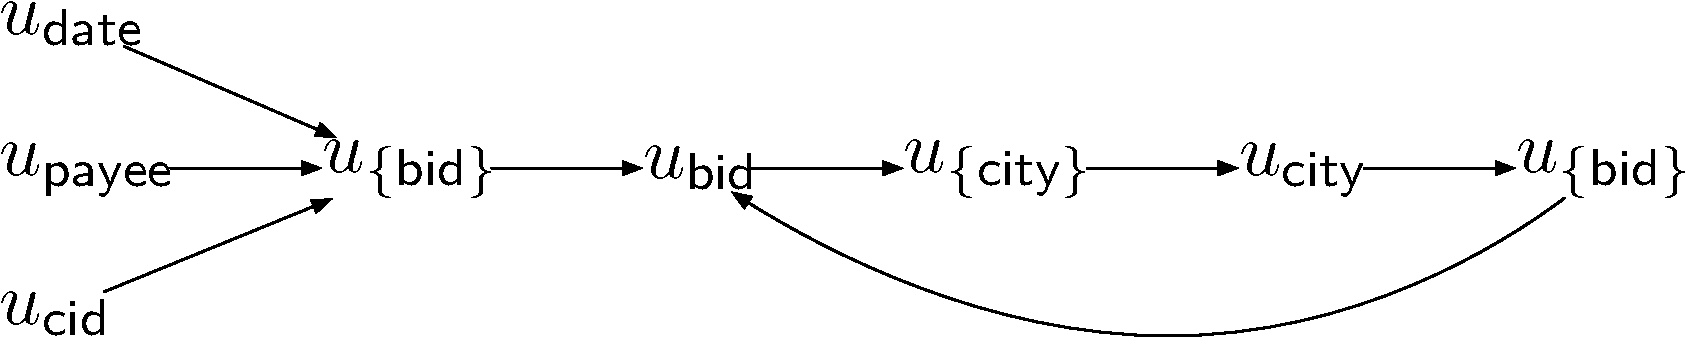
\includegraphics[width=1\columnwidth]{fig/schemagraph.pdf}
\vspace{-2.7ex}
\caption{The schema graph of $\kb{\R}_{Q_{1}}$ (\ie
  $\kb{\R}_{4}$) \label{fig-schemagraph}}
\vspace{-2.7ex}
\end{figure}

\begin{example}\label{exa-schemagraph}
\revise{When $\kb{\A} = \kb{\R}_{2}$, the  schema graph of \bs $\kb{\R}_{Q_{1}}$
(\ie $\kb{\R}_{4}$) for query $Q_{1}$} is depicted in
Fig.~\ref{fig-schemagraph}. The graph is cyclic.
%The schema graph of \bs $\kb{\R}_{Q_{1}}$ (\ie $\kb{\R}_{4}$) for
%$Q_{1}$ with the set $\kb{\A} = \kb{\R}_{2}$ is depicted in
%Fig.~\ref{fig-schemagraph}. The graph is cyclic.
\end{example}


\eetitle{Acyclicity}. We now formalize acyclicity.
We say that $\kb{\R}_{Q}$ is {\em acyclic \wrt $\kb{\R}_{o}$} if its schema
graph $G_{\kb{\R}_{Q}}$ is acyclic; otherwise $\kb{\R}_{Q}$ is
{\em cyclic}. Query $Q$ is {\em acyclic} \wrt $\kb{\R}_{o}$ if
$\kb{\R}_{Q}$ is acyclic \wrt $\kb{\R}_{o}$. A query load $\Q$ is
{\em acyclic} \wrt $\kb{\R}_{o}$ if each query in $\Q$ is acyclic \wrt
$\kb{\R}_{o}$.


\vspace{0.8ex}
Algorithm \opts checks whether $\Q$ is acyclic \wrt the optimal
solution $\kb{\R}_{o}$ to ILP-(I), and returns $\kb{\R}_{o}$ 
if $\Q$ is acyclic (line~\ref{opts-l2}). %However,

If $\Q$ is
cyclic, $\kb{\R}_{o}$ may not be optimal since the ILP-(I) cannot
capture the scan-free evaluability of $\kb{\R}_{o}$. \revise{If so,
%for such cases, \opts %further
\opts triggers ILP-(II)}. %below.


\vspace{0.36ex}

\stitle{(3) ILP-(II)}.
For cyclic queries,
ILP-(II) computes %only
\ssf-optimal normalized \bds $\kb{\R}_{o}'$ for $\Q$. 
To do so, ILP-(II) %is almost the same as ILP-(I) except that it
extends ILP-(I) with an additional constraint besides the constraints
of ILP-(I):\looseness=-1
\vspace{-0.7ex}
\begin{alignat}{2}                                                       
&  y_{\kb{R}}^{Q} = 0 &~~~~~~~~~~~~\forall \kb{R}, \forall Q, X_{\kb{R}}\not\subseteq P_{Q}
\end{alignat}                                                            

\vspace{-0.7ex}

Intuitively, equation (11) allows ILP-(II) to enforce that when
selecting \bss to make query $Q$ scan-free, for each
\bs $\kb{R} \ak = \ak \bschema{X}{Y}$ it picks for $Q$, $X\subseteq
P_{Q}$, \ie $Q$ can be answered with $\get(k)$ operations where keys 
$k$ are \revise{among} the parameters of $Q$.
%\looseness = -1


\vspace{0.36ex}
When $\Q$ is cyclic \wrt the \bds $\kb{\R}_{o}$,
%encoded by the optimal solution to ILP-(I),
algorithm \opts constructs and solves
ILP-(II), and returns the \bds $\kb{\R}_{o}'$ encoded by the
optimal solution to ILP-(II), \ie $\kb{\R}_{o}'$ consists of \bss
$\kb{R}$ in $\kb{\A}$ with $y_{\kb{R}} = 1$. 

\begin{example}\label{exa-ILP-II}
With $\kb{\R}_{3}$, \opts computes an optimal assignment to
ILP-(II) that has $z_{Q} = 0$, %$x_{\at{city}} = 0$,
$y_{\kb{\at{TC}}_{1}} = y_{\kb{\at{B}}_{1}} = 1$ and
$y_{\kb{\at{B}}_{2}} = y_{\kb{\at{C}}_{1}} = 0$. %, which
This encodes a
\bds $\kb{\R}_{5}$ consisting of $\kb{\at{B}}_{1}$ and
$\kb{\at{TC}}_{1}$ for query load $\Q$. %With this, assignment,
%Note that
The objective of ILP-(II) %with this assignment
is 1.06, which is
consistent with $f_{0}(\Q,
\kb{\R}_{5})$. 
\end{example}

\vspace{-0.4ex}

\stitle{Analysis}. We next prove Theorem~\ref{thm-opts} with the following lemmas. 



\begin{lemma}\label{lem-ILP-norm}
  For any \SQL $Q$, if for each \qcs $W$ in $\Wc_{Q}$, there
  exists a \bs $\kb{R}$ in $\kb{\R}$ that supports $W$, then
  $\kb{\R}$ is in the normal form for $Q$.
\end{lemma}
\looseness = -1

\revise{The proof of}
Lemma~\ref{lem-ILP-norm} is straightforward from the following observations:
(a) a query $Q$ can be answered if all of its \qcs values can be
retrieved; moreover,
(b) if a \qcs $W$ is supported by a \bs $\kb{R}$, then by scanning
$\kb{R}$ one could retrieve all the $W$-values. 

%Note that
The condition of Lemma~\ref{lem-ILP-norm} is enforced
by inequation (8) for each query $Q$ in $\Q$.
Hence, by Lemma~\ref{lem-ILP-norm}, any feasible solution to ILP-(I)
or ILP-(II) %must
encodes a \bds %that is
in the normal form for $\Q$
%This verifies
(Theorem~\ref{thm-opts}(1)). 


\vspace{1ex}
For feasible solutions to ILP-(I) and ILP-(II) and the
corresponding \bdss $\kb{\R}$ encoded by them,
we have the following.

\vspace{-0.5ex}
\begin{lemma}\label{lem-ILP}
  For any K-FK join \SPC query $Q$ in $\Q$, 
\mbi
\item[(1)] $Q$ is scan-free over some \bds $\kb{\R}$
only if there exists a feasible
  solution to ILP-(I) with $z_{Q} = 1$;
\item[(2)] $Q$ is scan-free evaluable over $\kb{\R}$
  if there is a \bds $\kb{\R}$ encoded by a feasible
  solution to ILP-(I) with $z_{Q} = 1$ and $Q$ is acyclic \wrt
  $\kb{\R}$; %and
\item[(3)] $Q$ is strongly scan-free evaluable iff there exist a
  feasible solution to ILP-(II) with $z_{Q} = 1$.
\mei
\vspace{-3ex}
\eat{%EAT
  \sstab (1) $Q$ is scan-free over some \bds $\kb{\R}$ only if there exists a feasible
  solution to ILP-(I) with $z_{Q} = 1$; 

  \sstab (2) $Q$ is scan-free evaluable over $\kb{\R}$
  if there is a \bds $\kb{\R}$ encoded by a feasible
  solution to ILP-(I) with $z_{Q} = 1$ and $Q$ is acyclic \wrt
  $\kb{\R}$; and

  \sstab (3) $Q$ is strongly scan-free evaluable iff there exist a
  feasible solution to ILP-(II) with $z_{Q} = 1$.
  }%EAT
\end{lemma}

\vspace{-0.7ex}

\warn{Clarify the difference between (1) and (2). 
Isn't scan-free and scan-free evaluable the same (Section~2)?
Don't expect the reader to remember the subtle notions
at this point}

\begin{proofS}
% All three results can be proved by induction on $(m, n, p)$,
% where $m$ is $\cdd{\Q}$, \ie the number of $z_{Q}$ variables; $n$
% is the number of $x_{A}^{Q}$ variables; $p$ is the number of
% $y_{\kb{R}}$ variables, \ie the number of \bss in $\kb{\R}$.
%In particular, to prove (1), the key observation for the
%induction is the following:
%All
The three results can all be proved by induction. 
%In particular,
%To prove
For (1), observe that when $Q$ is scan-free
over some \bds $\kb{\R}$, by definition there must exist a chain
(\ie plan)
of \get operations that %can
retrieve \revise{attribute}
$A$ from parameters of $Q$
for each $A\in Y_{Q}$. One can verify by induction on the length
of the chain that each chain encodes a partial assignment to the
0/1-variables that satisfies the constraints of ILP-(I) and leads to
$x_{A}^{Q} = 1$ for each $A\in Y_{Q}$. By inequation (3), such
partial assignments, together with $z_{Q} = 1$, form a feasible
solution (\ie assignment) that satisfies all the constraints
in ILP-(I).

One can verify
(2) along the same lines. By induction on $(m, n)$,
where $m$ is the number of $x_{A}^{Q}$ variables and $n$ is the
number of $y_{\kb{R}}$ variables (\ie the number of \bss in
$\kb{\A}$) in ILP-(I), one can construct a scan-free query plan
over $\kb{\R}$ from the assignment of any feasible solution. The
key step is that when $Q$ is acyclic \wrt $\kb{\R}$, for each
$x_{A}^{Q} = 1$ for some $A\in Y_{Q}$, one can always trace back
to $x_{A'}^{Q} = 1$ for some parameters $A\in P_{Q}$, such that
the trace encodes a fetching plan for $A$ from $A'$.
For (3), the if (resp.~only if) direction follows from the proof
of (2) (resp.~(1)), and is simpler. 
\end{proofS}
\looseness = -1

\eat{%EAT DOES MORE HARM THAN GOOD
Lemma~\ref{lem-ILP} considers \SPC queries with K-FK joins 
since all the analysis is based on that $Q$ is
(resp.~strongly) scan-free iff $\bschema{P_{Q}}{Y_{Q}}$ is
implied by $\kb{\R}$, \ie there exists a (resp.~strongly) scan-free
plan over $\kb{\R}$ that fetches attributes in $Y_{Q}$ over
$\kb{\R}$, starting from $P_{Q}$. Such a prerequisite holds for
\SPC queries in which joins are all K-FK joins.
\looseness = -1}%EAT

Putting these together, we are now ready to prove
  Theorem~\ref{thm-opts}.

\vspace{0.8ex}
\noindent
    {\bf Proof of Theorem~\ref{thm-opts}}. As remarked earlier,
    Theorem~\ref{thm-opts}(1) follows from Lemma~\ref{lem-ILP-norm}.
To show  Theorem~\ref{thm-opts}(2a), observe that
by Lemma~\ref{lem-ILP}(1), feasible solutions to ILP-(1) can
cover all \bdss over which $Q$ is scan-free. This ensures that
the \bds $\kb{\R}_{o}$ encoded by the optimal solution to ILP-(1)
must have the minimum ranking score.
%, although its ``true''
%score of $\usf(\Q,\ak \kb{\R}_{o})$ (\ie~measure (1)) may be worse.
Lemma~\ref{lem-ILP}(2) ensures that if $\Q$ is
acyclic \wrt $\kb{\R}_{o}$ then its score of $\usf(\Q,\ak
\kb{\R}_{o})$ is measured correctly in the optimal solution to
ILP-(I); hence $\kb{\R}_{o}$ is the optimal \bds for $\Q$. This
verifies Theorem~\ref{thm-opts}(2a).
%\looseness = -1

\vspace{0.6ex}
For Theorem~\ref{thm-opts}(2b),
Lemma~\ref{lem-ILP}(3) tells us that feasible solutions to
ILP-(II) can encode all \bdss over which $\Q$ is strongly
scan-free, \ie the \bds $\kb{\R}_{o}'$ encoded by the optimal
solution to ILP-(II) is measured correctly
%\wrt all the measures via the ILP program
when the strong scan-free evaluability is
adopted. Hence, $\kb{\R}_{o}'$ must always be \ssf-optimal for
$\Q$. This verifies Theorem~\ref{thm-opts}(2b). \eop
\looseness = -1


\eetitle{Complexity}. Algorithm \opts is in
$O(\cd{\kb{\A}}\cd{\Q} + T_{\at{ILP}} )$-time, where
$\cd{\kb{\A}}$ and $\cd{\Q}$ are the total number of attributes
in $\kb{\A}$ and $\Q$ (in the predicates of its algebra form),
respectively, and $T_{\at{ILP}}$ is the time for solving the ILP programs. 
Indeed, %note the following:
(a) it takes $O(\cd{\Q}\cd{\kb{\A}})$ time to construct ILP-(I) and
ILP-(II) with $\kb{\A}$.
(b) There are $\cdd{\Q} + \cdd{\Q}\cd{\A} + \cdd{\kb{\R}} + \cdd{\kb{\A}}\cdd{\Q}$ 0/1
variables in both ILP programs.
(c) ILP-(II) and ILP-(I) have at most
$3\cdd{\Q}\cdd{\kb{\A}} + 5\cdd{\Q}\cd{\R} + \cd{\Q} +
\cdd{\Q} + \cdd{\kb{\A}} + \cd{\kb{\A}}\cdd{\Q}$ linear
constraints, where $\cd{\R}$ is the total number of attributes in
$\R$, $\cdd{\Q}$ is the number of queries in $\Q$ and
$\cdd{\kb{\A}}$ is the number of \bss in $\kb{\A}$.\looseness=-1 



\stitle{Remark}. Algorithm \opts is generic and can be easily
adapted to serve various scenarios. Below are a few examples.

\sstab (1) One can treat some of the measures of \opts
as constraints. For instance, if users
want to find optimal normalized \bds with size bounded by a
storage budget $B$, then they can simply move $f_{3}$ from the
objective (1) of ILP-(I) and ILP-(II) to a constraint 
$f_{3}\leq B$.

\sstab (2) One can even specify certain queries $Q$ and request
to make them scan-free over the returned \bds $\kb{\R}$. This is
easily done by adding additional constraints $z_{Q} = 1$
for the pick queries.

\sstab (3) By controlling $c_{i}$ in the rank aggregate function
$f(\Q, \kb{\R})$, one can prioritize certain
measures \revise{of their applications}. 
For example, if users care more about the
  performance of query answering than
  %while downplaying
the maintenance cost, \eg when querying static historical data,
they could assign $c_{1}$ a
  large coefficient, %followed by a moderate $c_{2}$,
  and set $c_{4}$
to 0.

\eat{%EAT
  \section{Selecting top-$k$ Optimal Schemas}
\label{sec-select}

In light of Theorem~\ref{thm-complexity}, any efficient solution
to \bdsd is necessarily approximate.
Nonetheless, below we develop a practical algorithm for \bdsd
that can compute, given any universe set $\kb{\A}$ of \bss,
the optimal \bds $\kb{\R}$ for $\Q$ that is subsumed by
$\kb{\A}$. Hence, whenever $\kb{\A}$ subsumes the optimal
$\kb{\R}$ for $\Q$, the algorithm can identify and return it from
$\kb{\A}$.

Below we present the algorithm with a given universe set $\kb{\A}$.
We will study the construction of $\kb{\A}$ in
Section~\ref{sec-cover}.



\begin{myfloat}[t]
\vspace{1.2ex}
\begin{minipage}{0.50\textwidth}
  \removelatexerror
%%%%%%%%%%%%%%%%%%%%% Algorithm: OPTS
{\scriptsize
\setlength{\floatsep}{0cm} % set blank space above the figure
\setlength{\textfloatsep}{-2cm}% set blank space below the figure
\IncMargin{1em}
\vspace{-0.7ex}
\begin{algorithm}[H]
\setstretch{1.1}
%\SetAlgoNoLine
\Indentp{-2ex}
%\DontPrintSemicolon
%\SetAlgoLined
\KwIn{$\Q$ over $\R$, set $\kb{\A}$ of \bss, rank aggregate function $f$.}
\KwOut{\bds $\kb{\R}$ in normal form for $Q$ with minimum $f(\Q,
  \kb{\R})$ among all normalized \bdss subsumed by $\kb{\A}$.}
\Indentp{1em}
\BlankLine
construct and solve ILP-(I) with
$\kb{\A}$\label{opts-l1}\tcp*[r]{denote its answer by $\kb{\R}_{o}$}
\lIf{$\Q$ is {\em acyclic} \wrt $\kb{\R}_{o}$}{\Return $\kb{\R}_{o}$\label{opts-l2}}
\Else{
  construct and solve ILP-(II) with $\kb{\A}$\label{opts-l4}
  \tcp*[r]{let $\kb{\R}'_{o}$ be its answer}
  \Return $\kb{\R}'_{o}$ \;\label{opts-l5}
}
\caption{Algorithm \opts\label{alg-opts}} 
\end{algorithm}
\DecMargin{1em}
}
%%%%%%%%%%%%%%%%%%%%%
\end{minipage}
\vspace{-2.4ex}
\end{myfloat}


The algorithm, denoted by \opts and shown as
Algorithm~\ref{alg-opts}, takes as input a query load $\Q$ over
database schema $\R$, a set $\kb{\A}$ of \bss and an aggregate rank
function $f(\Q,\ak \kb{\R})$.
It computes the optimal \bds $\kb{\R}$ normalized for $\Q$ from $\kb{\A}$,
\ie for any other \bds $\kb{\R}'\ak \subseteq \ak \kb{\A}$ that is in
normal form for $\Q$, $f(\Q,\ak \kb{\R})\ak \leq\ak f(\Q,\ak \kb{\R}')$.
%
Its core idea is to use integer linear programming (ILP) to
express the normal form conditions and ranking measures of \bdss
for $\Q$, so that computing the optimal normalized \bds in
$\kb{\A}$ reduces to solving an ILP program. This allows us to
employ the latest advances of ILP, \eg algorithms
(cf.~\cite{ILPbook}) and commercial ILP
solvers~\cite{cplex,gurobi,XpressMP}.


This is challenging since both (a) the normal form and (b) the
scan-free evaluability of \bdss for $\Q$ are semantically defined
and may not be able to directly encoded by an ILP.
% Indeed, (a) is already \NP-hard for generic \SPC queries and
% cannot be exactly captured by linear functions, \eg ILP.

\vspace{1ex}
Nonetheless, \opts guarantees the following. We say that
a \bds $\kb{\R}$ normalized for $\Q$ is {\em \ssf-optimal}
({\em strongly scan-free optimal}) \wrt $\kb{\A}$ if $f(\Q, \kb{\R})$
concerns strongly scan-free queries, \ie $\kb{\R}$ is optimal
among all normalized \bdss when $f(\Q, \kb{\R})$ uses strongly
scan-free to for measure (1): $\sf(Q,\ak \kb{\R}) \ak = \ak 1$
iff $Q$ is strongly scan-free over $\kb{\R}$. We say an \SPC
query $Q$ is a key-foreign key (K-FK) join query if all joins in
$Q$ are K-FK joins.
\looseness = -1

\vspace{-0.3ex}
\begin{theorem}\label{thm-opts}
Algorithm \opts guarantees to compute $\kb{\R}$ from $\kb{\A}$
for $\Q$ such that
(1) $\kb{\R}$ is always in normal form for $\Q$; and
(2) if $\Q$ consists of K-FK join \SPC queries only, then
\bi
\item[(a)] $\kb{\R}$ is optimal among all \bdss from $\kb{\A}$
  if $\Q$ is {\em acyclic}; 
\item[(b)] $\kb{\R}$ is \ssf-optimal when $\Q$ is cyclic. 
\ei
\vspace{-3.5ex}
\end{theorem}

We will elaborate the {\em acyclicity} of $\Q$ shortly.

Algorithm \opts computes $\kb{\R}$ via two ILP programs,
referred to as ILP-(I) and ILP-(II).
It constructs and solves ILP-(I) (line~\ref{opts-l1}),
via whose answer it decides whether $\Q$ is acyclic and
returns the \bds encoded in the solution to ILP-(I) if so
(line~\ref{opts-l2}), which is the optimal normalized \bds from
$\kb{\A}$ for \SPC with K-FK joins only
(Theorem~\ref{thm-opts}(a)). 
If it identifies that $\Q$ is cyclic, it then constructs and
solves ILP-(II) and returns the \bds encoded in its solution
(lines~\ref{opts-l4}-\ref{opts-l5}), which is the \ssf-optimal
normalized \bds from $\kb{\A}$ for \SPC with K-FK joins
(Theorem~\ref{thm-opts}(b)).
\looseness = -1


\vspace{0.8ex}
Below we present the two ILP programs and show how \opts
identifies acyclic queries $\Q$. 


\stitle{(a) ILP-(I)}. 
ILP-(I) uses the following 0/1-variables: 
(a)~For each query $Q\in \Q$ , we use $z_{Q}$ to indicate whether
$z_{Q}$ is scan-free over $\kb{\R}$ or not:
$z_{Q} = 1$ indicates we pick \bss for $\kb{\R}$ over which $\Q$ is scan-free.
(b)~For each query $Q\in \Q$ and attribute $A$ in $Q$, we use
$x_{A}^{Q}$ to indicate whether $A$ is fetchable from constants
in $Q$ over $\kb{\R}$. 
(c)~For each \bs $\kb{R}$, we use $y_{\kb{R}}$ to indicate
whether $\kb{R}$ is picked for $\kb{\R}$, and use $y^{Q}_{\kb{R}}$ to
indicate whether $\kb{R}$ is picked in order to make $Q$ scan-free
for each $Q\in \Q$.
\looseness = -1

\vspace{0.4ex}
We also use the following notations. For a \bs $\kb{R}$,
denote by $X_{\kb{R}}$ and $Y_{\kb{R}}$ the attributes such that
$\kb{R}\ak =\ak  \bschema{X_{\kb{R}}}{Y_{\kb{R}}}$.
We use $A$ to denote an attribute and use $R$ to denote a
relation schema in $\R$.
Denote by $\A_{R}$ the set of \bss $\kb{R} \ak = \ak
\bschema{X}{Y}$ with $Y$ from relation schema $R$. For an
attribute $A$ of $\R$, denote by $\RHS(A)$ the set of all \bss
$\kb{R}$ in $\kb{\A}$ such that $A\in Y_{\kb{R}}$.
%
For each parametric query $Q$ in $\Q$, denote by $P_{Q}$ the set
of parameters of $Q$; denote by $Y_{Q}$ all the other
attributes appeared in the predicates of $Q$ that is in relational
algebra form (\ie $Y_{Q}$ includes attributes appeared
in joins or project predicates of $Q$). 
\looseness = -1

For each $Q$ in $\Q$ and each relation $R$ in $Q$, denote by
$W_{R}$ the \qcs~\cite{blinkdb} of $Q$ on $R$ (\ie attributes of
$R$ that are also in $P_{Q}Y_{Q}$ of $Q$); denote by $\Wc_{\Q}$
the set of all \qcs of queries in $\Q$. For each \qcs $W$ in
$\Wc_{\Q}$, denote by $\kb{\R}_{W}$ the set of \bss $\kb{R}\ak
=\ak \bschema{X}{Y}$ in $\kb{\A}$ that {\em support} $W$: $W\ak\subseteq\ak XY$. 

% As will be shown shortly, if all \qcs of a query $Q$ are
% supported by a set $S$ of \bss, then $S$ is a cache database
% schema that is in normal form for $Q$.

Then program ILP-(I) is constructed as follows.

\begin{tcolorbox}[
  blanker,
  breakable,
  ]
  \begin{alignat}{2}
\hspace{-1.25cm}\text{minimize: } & c_{1}f_{1}+c_{2}f_{2}+c_{3}f_{3}+c_{4}f_{4}~~~~~~~~  &  
  \end{alignat} 
  \begin{alignat}{2}
   \hspace*{-0.15cm}\text{subject to: }&  x_{A}^{Q} = 1 & \forall
    A\in P_{Q}, \forall Q \\[0.8ex] 
    & z_{Q}\leq x_{A}^{Q} & \forall A \in Y_{Q},\forall Q \\[0.8ex]
    & x_{A}^{Q} \leq\textstyle \sum_{\kb{R}\in \RHS(A)}\!y_{\kb{R}}^{Q} &~\forall
    A\not\in P_{Q}, \forall Q \\[0.8ex]
    & y_{\kb{R}}^{Q} \leq x_{A}^{Q} & \forall \kb{R}\in \kb{\A}, \forall A\in X_{\kb{R}}, \forall
    Q\\[0.8ex]
    & \textstyle \sum_{\kb{R}\in \A_{R}} y_{\kb{R}}^{Q} \leq 1 & 
    \forall R\in \R, \forall Q \\[0.8ex]
    & y_{\kb{R}}^{Q} \leq y_{\kb{R}} & \forall Q, \forall \kb{R} \\[0.8ex]
    & \textstyle\sum_{\kb{R}\in \kb{R}_{W}} y_{\kb{R}} \geq 1 & \forall W\in \Wc_{\Q} \\[0.8ex]
    %& x_{A}^{Q} \in \{0, 1\} & \forall A\text{ in }\R, \forall
    %Q\\[0.8ex]
    & z_{Q}, x_{A}^{Q} \in \{0, 1\} & \forall
    A\text{ in }\R, \forall Q\\[0.8ex]
    & y_{\kb{R}}, y_{\kb{R}}^{Q} \in \{0, 1\} & \forall Q, \forall
    \kb{R} 
  \end{alignat} 
\end{tcolorbox}

\sstab
where $c_{i} (i\in[1, 4])$  in (1) are coefficients adjustable by the users when specifying the
optimization objective and $\sum_{i=1}^{4}c_{i} = 1$ (recall
from Section~\ref{sec-rank}), and $f_{i}(i\in [1, 4])$ are:

\begin{tcolorbox}[
  blanker,
  breakable,
  ]
\mat{0ex}{
$f_{1} = \textstyle\sum_{Q\in \Q} (1-z_{Q})*w_{Q}$ ~~~~~\= $f_{2} = \textstyle\sum_{\kb{R}\in \kb{\A}} y_{\kb{R}}*|Y_{\kb{R}}|$\\[0.5ex]
$f_{3} = \textstyle\sum_{\kb{R}\in \kb{\A}} y_{\kb{R}}*\esize(\kb{R})$
\> $f_{4} = \sum_{\kb{R}\in\kb{\A}} y_{\kb{R}}*\Pi_{R\in \Mc_{\kb{R}}}f_{R}$}
%(recall $\update(\Q,\A)$  in Sec.~\ref{sec-rank})}
\end{tcolorbox}

Intuitively, equation (2) of the ILP program indicates that all
attributes in $P_{Q}$ are ``known'' for $Q$ already; to make
$Q$ scan-free, we need to fetch $Y_{Q}$-values (partial tuples) associated
with such known $P_{Q}$-values via selected \bss for
$Q$, which are indicated by $y_{\kb{R}}^{Q}$.
Inequation (3) ensures that when a query $Q$ is made scan-free (\ie
$z_{Q} = 1$), all attributes in $Y_{Q}$ should be also be
{\em fetchable}, where an attribute is fetchable in $Q$
when it can be retrieved from $P_{Q}$ via $\get(k)$ over picked
\bss without scans.
\looseness = -1

Inequation (4) enforces that, when an attribute $A$ is fetchable in
$Q$ (\ie $X_{A}^{Q} = 1$), $A$ must either in $P_{Q}$ or $A$ is
in $Y_{\kb{R}}$ of some \bs $\kb{R}$ ($\kb{R} \in \RHS(A))$
that has been picked for $Q$, \ie $y_{\kb{R}}^{Q} = 1$.
Inequation (5) further enforces that attribute $A$ in $X_{\kb{R}}$
of $\kb{R}$ in $Q$ must be fetchable if $\kb{R}$ is picked for $Q$.

Inequation (6) is to ensure that for each relation $R$ in $\R$,
only one \bs $\kb{R} \ak =\ak \bschema{X}{Y}$ with $Y$ from $R$ is used
to make $Q$ scan-free; this is to ensure that, when all $Y_{Q}$ attributes
can be fetched from $P_{Q}$-values, they are warranted to come from
the same tuples in the database instance $\D$ of $\R$, \ie their
combinations do not generate ``false'' $Y_{Q}$-values that are
not in $\D$.
\looseness = -1

The ILP constraints (2)-(6) together ensure that if $z_{Q}\ak
=\ak 1$, \ie $Q$ is scan-free over \bss $\kb{R}$ picked for $Q$
($y_{\kb{R}}^{Q}\ak =\ak 1$), for each attribute $A$ in $Y_{Q}$,
there must exist a sequence of \get operations that can retrieve
$A$ over the picked \bss starting from parameters $P_{Q}$ of $Q$
(assuming the picked \bss are ``acyclic'', which we will
elaborate shortly).


Inequation (7) ensures that, when $Q$ picks a \bs $\kb{R}$
($y_{\kb{R}}^{Q} = 1$), $\kb{R}$ is included in \bds $\kb{\R}$
($y_{\kb{R}} = 1$).

Inequation (8) is to guarantee that any feasible solution to the
ILP program must yield a \bds that is in normal form for all
queries in $\Q$: for each \qcs $W$ of $\Q$, $W$ is supported by
at least a \bs picked in $\kb{\R}$. 

Equations (9)-(10) claim that all variables are either 0 or 1.


\vspace{0.8ex}
Algorithm \opts constructs and solves ILP-(I), 
by using existing ILL solvers, \eg Gurobi~\cite{gurobi} or
IBM CPLEX~\cite{cplex}, which can solve, \eg ILP 
with 23,000 decision variables and 4,000  constraints
in less than a minute~\cite{ILPstat}.
%
It then interprets \bdss from solutions to the ILP
program: for any feasible solution (\ie 0/1 assignment to the
variables), it construct \bds $\kb{\R}$ that consists of \bss
$\kb{R}$ in $\kb{\A}$ with $y_{\kb{R}}  = 1$ in the feasible
solution. We also refer to such $\kb{\R}$ the \bds encoded by the
solution to ILP program. \opts returns the \bds
$\kb{\R}_{o}$ encoded by the optimal solution to ILP-(I) only
when $\Q$ is acyclic \wrt $\kb{\R}_{o}$ (line~\ref{opts-l2}), which we elaborate below. 



\stitle{(b) Acyclicity checking}. We first exemplify the notion
of acyclicity of a query $Q$ \wrt the \bds $\kb{\R}_{o}$ encoded
in the optimal solution to ILP-(I). Let $\kb{\R}_{Q}$ be the set
of \bss $\kb{R}$ in $\kb{\R}_{o}$ with $y_{\kb{R}}^{Q} = 1$ in
the solution to ILP-(I).


\begin{example}\label{exa-acyclicity}
Illustrate acyclic \bs can't ensure $A$ is fetchable even
$x_{A}^{Q} = 1$. Motivate the need for acyclic checking.
\end{example}

As shown in Example~\ref{exa-acyclicity}, if $\kb{\R}_{Q}$ is
``acyclic'', attribute $A$ in $Y_{Q}$ of $Q$ cannot always be
fetched from parameters $P_{Q}$ of $Q$ even $x_{A}^{Q} = 1$,
where $\kb{\R}_{Q}$ consists of all \bss $\kb{R}$ in $\kb{\R}_{o}$
with $y_{\kb{R}}^{Q} = 1$ in the solution to ILP-(I).
In other words, ILP-(I) cannot capture the scan-free
evaluability of $\kb{\R}_{Q}$ and hence it may not be optimal anymore. 


We next formalize the acyclicity of \bds $\kb{\R}_{Q}$ for $Q$.
% As will be shown shortly, if $\A_{Q}$ in $\A$ identified
% by the ILP program is acyclic for each $Q$ in $\Q$, \opts safely
% returns $\A$ as the optimal \cds for $\Q$.
This is based on a graph representation of $\kb{\R}_{Q}$, referred to
as the {\em schema graph} of $\kb{\R}_{Q}$ and denoted by
$G_{\kb{\R}_{Q}}$.


\eetitle{Schema graph}. More specifically, $G_{\kb{\R}_{Q}}$ is a
directed graph constructed from $\kb{\R}_{Q}$ as follows: each \bs
$\kb{R} = (X\ra Y)$ is represented in $G_{\kb{\R}_{Q}}$ as $|X|+|Y|+1$
nodes and $|X|+|Y|$ edges:
\looseness = -1

\bi
\item each attribute $A$ in $X$ and $Y$ is a node $u_{A}$ in $G_{\kb{\R}_{Q}}$;
\item $G_{\kb{\R}_{Q}}$ additionally encodes set $Y$ as a node $u_{Y}$
\item $(u_{A}, u_{Y})$ is an edge in $G_{\kb{\R}_{Q}}$ for each $A\in X$; and
\item $(u_{Y}, u_{A})$ is an edge in $G_{\kb{\R}_{Q}}$ for each attribute $A\in Y$.
\ei 


\begin{example}\label{exa-schemagraph}
\end{example}


\eetitle{Acyclicity}.
We say that $\kb{\R}_{Q}$ is acyclic \wrt $\kb{\R}_{o}$ if schema
graph $G_{\kb{\R}_{Q}}$ is acyclic; otherwise $\kb{\R}_{Q}$ is
called cyclic. Query $Q$ is acyclic \wrt $\kb{\R}_{o}$ if
$\kb{\R}_{Q}$ is acyclic \wrt $\kb{\R}_{o}$. A query load $\Q$ is
acyclic \wrt $\kb{\R}_{o}$ if each query in $\Q$ is acyclic \wrt
$\kb{\R}_{o}$.


\vspace{0.8ex}
Algorithm \opts checks whether $\Q$ is acyclic \wrt the optimal
solution $\kb{\R}_{o}$ to ILP-(I), and returns $\kb{\R}_{o}$ 
if $\Q$ is acyclic (line~\ref{opts-l2}). However, if $\Q$ is
cyclic, $\kb{\R}_{o}$ may not be optimal since the ILP-(I) cannot
capture the scan-free evaluability of $\kb{\R}_{o}$;
for such cases, \opts uses ILP-(II) below.



\stitle{(c) ILP-(II)}.
To tackle the issue caused by scan-free evaluability for cyclic
query workload in ILP-(I), ILP-(II) instead computes %only
\ssf-optimal normalized \bds $\kb{\R}_{o}'$ for $\Q$. 
To do so, ILP-(II) is almost the same as ILP-(I) except that it
extends ILP-(I) with an additional constraint:
\begin{alignat}{2}                                                       
&  y_{\kb{R}}^{Q} = 0 &~~~~~~~~~~~~\forall \kb{R}, \forall Q, X_{\kb{R}}\not\subseteq P_{Q}
\end{alignat}                                                            

Intuitively, equation (11) allows ILP-(II) to enforce that, when
selecting \bss to make query $Q$ scan-free, for each
\bs $\kb{R} \ak = \ak \bschema{X}{Y}$ it picks for $Q$, $X\subseteq
P_{Q}$, \ie $Q$ can be answered with $\get(k)$ operations where
$k$ are the parameters of $Q$. 
\looseness = -1


\vspace{0.8ex}
When $\Q$ is cyclic \wrt the \bds $\kb{\R}_{o}$ encoded by the
optimal solution to ILP-(I), algorithm \opts constructs and solves
ILP-(II), and returns the \bds $\kb{\R}_{o}'$ encoded by the
optimal solution to ILP-(II), \ie $\kb{\R}_{o}'$ consists of \bss
$\kb{R}$ in $\kb{\A}$ with $y_{\kb{R}} = 1$. 

\begin{example}\label{exa-opts}
\end{example}



\stitle{Analysis}. We next prove Theorem~\ref{thm-opts} with the following lemmas. 



\begin{lemma}\label{lem-ILP-norm}
  For any \SQL query $Q$, if for each \qcs $W$ in $\Wc_{Q}$ there
  is a \bs $\kb{R}$ in $\kb{\R}$ that supports $W$, then
  $\kb{\R}$ is in normal form for $Q$. 
\end{lemma}

Lemma~\ref{lem-ILP-norm} is straightforward from the following observations:
(a) a query $Q$ can be answered if all of its \qcs values can be
retrieved; moreover,
(b) if a \qcs $W$ is supported by a \bs $\kb{R}$, then by scanning
$\kb{R}$ one could retrieve all the $W$-values. 

Note that the condition of Lemma~\ref{lem-ILP-norm} is enforced
by inequation (8) for each $Q$ in $\Q$.
Hence, by Lemma~\ref{lem-ILP-norm}, any feasible solution to ILP-(I)
or ILP-(II) must encode a \bds that is in normal form for $\Q$.
This verifies Theorem~\ref{thm-opts}(1). 


\vspace{1ex}
Consider feasible solutions to ILP-(I) and ILP-(II) and the
corresponding \bdss $\kb{\R}$ encoded by them.

\vspace{-0.5ex}
\begin{lemma}\label{lem-ILP}
  For any K-FK join \SPC query $Q$ in $\Q$, 

  \sstab (1) $Q$ is scan-free over some \bds $\kb{\R}$ only if there exists a feasible
  solution to ILP-(I) with $z_{Q} = 1$; 

  \sstab (2) if there exists a \bds $\kb{\R}$ encoded by a feasible
  solution to ILP-(I) with $z_{Q} = 1$ and $Q$ is acyclic \wrt
  $\kb{\R}$, then $Q$ is scan-free evaluable over $\kb{\R}$; and

  \sstab (3) $Q$ is strongly scan-free evaluable iff there exist a
  feasible solution to ILP-(II) with $z_{Q} = 1$. 
\end{lemma}

\begin{proofS}
% All three results can be proved by induction on $(m, n, p)$,
% where $m$ is $\cdd{\Q}$, \ie the number of $z_{Q}$ variables; $n$
% is the number of $x_{A}^{Q}$ variables; $p$ is the number of
% $y_{\kb{R}}$ variables, \ie the number of \bss in $\kb{\R}$.
%In particular, to prove (1), the key observation for the
%induction is the following:
All three results can be proved by induction. 
In particular, to prove (1), observe that when $Q$ is scan-free
over some \bds $\kb{\R}$, by definition there must exist a chain
(\ie plan)
of \get operations that can retrieve $A$ from parameters of $Q$
for each $A\in Y_{Q}$. One can prove by induction on the length
of the chain that each chain encodes a partial assignment to the
0/1-variables that satisfies constraints of ILP-(I) and leads to
$x_{A}^{Q} = 1$ for each $A\in Y_{Q}$. By inequation (3), such
partial assignments, together with $z_{Q} = 1$, form a feasible
solution (\ie assignment) that satisfies all constraints in ILP-(I).
%
(2) is proved along the same lines. By induction on $(m, n)$,
where $m$ is the number of $x_{A}^{Q}$ variables and $n$ is the
number of $y_{\kb{R}}$ variables (\ie the number of \bss in
$\kb{\A}$) in ILP-(I), one can construct a scan-free query plan
over $\kb{\R}$ from the assignment of any feasible solution. The
key step is that, when $Q$ is acyclic \wrt $\kb{\R}$, for each
$x_{A}^{Q} = 1$ for some $A\in Y_{Q}$, one can always trace back
to $x_{A'}^{Q} = 1$ for some parameters $A\in P_{Q}$, such that
the trace encodes a fetching plan for $A$ from $A'$.
For (3), the if (resp. only if) direction follows from the proof
of (2) (resp. (1)), and is simpler. 
\end{proofS}
\looseness = -1

By Lemma~\ref{lem-ILP}(1), feasible solutions to ILP-(1) can
cover all \bdss over which $Q$ is scan-free. This ensures that
the \bds $\kb{\R}_{o}$ encoded by the optimal solution to ILP-(1)
must have optimal (minimum) ranking score, although its ``true''
score of $\usf(\Q,\ak \kb{\R}_{o})$ (\ie measure (1)) may be
worse. Lemma~\ref{lem-ILP}(2) ensures that, if $\Q$ is
acyclic \wrt $\kb{\R}_{o}$ then its score of $\usf(\Q,\ak
\kb{\R}_{o})$ is measured correctly in the optimal solution to
ILP-(I); hence $\kb{\R}_{o}$ is the optimal \bds for $\Q$. This
verifies Theorem~\ref{thm-opts}(2a).
\looseness = -1

Lemma~\ref{lem-ILP}(3) tells us that feasible solutions to
ILP-(II) can encode all \bdss over which $\Q$ is strongly
scan-free, \ie the \bds $\kb{\R}_{o}'$ encoded by the optimal
solution to ILP-(II) is measured correctly \wrt all the measures
via the ILP program when strong scan-free evaluability is
adopted. Hence, $\kb{\R}_{o}'$ must always be \ssf-optimal for
$\Q$. This verifies Theorem~\ref{thm-opts}(2b). 

Note that, \SPC queries with K-FK joins are assumed for
Lemma~\ref{lem-ILP} since all the analysis is based on that $Q$ is
(strongly) scan-free if and only if $\bschema{P_{Q}}{Y_{Q}}$ is
implied by $\kb{\R}$, \ie there exists a (strongly) scan-free
plan over $\kb{\R}$ that fetches attributes in $Y_{Q}$ over
$\kb{\R}$, starting from $P_{Q}$. Such a prerequisite holds for
\SPC queries of which the joins are all K-FK joins. 


\eetitle{Complexity}. Algorithm \opts is in
$O(\cd{\kb{\A}}\cd{\Q} + T_{\at{ILP}} )$-time, where
$\cd{\kb{\A}}$ and $\cd{\Q}$ are the total number of attributes
in $\kb{\A}$ and $\Q$ (in the predicates of its algebra form),
respectively, and $T_{\at{ILP}}$ is the time for solving the ILP programs. 
Indeed, note the following:
(a) It takes $O(\cd{\Q}\cd{\kb{\A}})$ time to construct ILP-(I) and
ILP-(II) with $\kb{\A}$.
(b) There are $\cdd{\Q} + \cdd{\Q}\cd{\A} + \cdd{\kb{\R}} + \cdd{\kb{\A}}\cdd{\Q}$ many 0/1
variables in both ILP programs.
(c) ILP-(II) (and hence ILP-(I)) has at most
$3\cdd{\Q}\cdd{\kb{\A}} + 5\cdd{\Q}\cd{\R} + \cd{\Q} +
\cdd{\Q} + \cdd{\kb{\A}} + \cd{\kb{\A}}\cdd{\Q}$ many linear
constraints, where $\cd{\R}$ is the total number of attributes in
$\R$, $\cdd{\Q}$ is the number of queries in $\Q$ and
$\cdd{\kb{\A}}$ is the number of \bss in $\kb{\A}$. 



\stitle{Remark}. Algorithm \opts is generic and can be easily
adapted to serve various scenarios. Below are a few examples.

\sstab (1) One can adapt \opts to treat some of the measures as
constraints. For instance, if one wants to find optimal \bds
with size bounded by $B$, then she can simply move $f_{3}$ from
the objective (1) of ILP-(I) and ILP-(II) to a constraint as
$f_{3}\leq B$.

\sstab (2) One can even specify certain queries $Q$ and request
to make them scan-free over the returned \bds $\kb{\R}$. This is
easily done by adding additional constraints $z_{Q} = 1$
for the pick queries.

\sstab (3) By controlling $c_{i}$ in the rank aggregate function
$f(\Q, \kb{\R})$, one can enforce priorities among the four
measures. For example, if one wants to favor performance while
downplaying the maintenance cost, she could assign $c_{1}$ a
large coefficient, following by moderate $c_{2}$, and set $c_{4}$
to 0.
}%EAT

\vspace{2ex}
%%%%%%%% Section 5 %%%%%%%%
\section{Computing Optimal Schema Cover}
\label{sec-cover}

We next develop an algorithm to construct a universe set
$\kb{\A}$ of \bss for $\Q$, as part of the input for algorithm
\opts above. %in Section~\ref{sec-select}.

\stitle{Algorithm}. The algorithm, denoted by \usc, takes as input a workload $\Q$
over a database schema $\R$, and returns a set $\kb{\A}$ of \bss
for $\Q$.
While there exist up to exponentially many distinct \bss for
$\Q$, \usc computes $\kb{\A}$ with the following properties:
\bi
\item[(a)] for each K-FK join \SPC query $Q\in \Q$, any rank aggregate function $f$,
  and any \bds $\kb{\R}_{Q}$ that is in the normal form for $Q$,
  if $\kb{\R}_{Q}$ is optimal under $f$, then
  $\kb{\R}_{Q}\subseteq \kb{\A}$; and
\item[(b)] the time for constructing $\kb{\A}$ is polynomial in
  $|\Q|$ and $|\R|$.
  %\footnote{We assume that the number joins in each $Q\in \Q$ is bounded by a constant.}
\ei
By (b), the size of $\kb{\A}$ is also polynomial in
$|\Q|$ and $|\R|$.

To do this, \usc constructs $\kb{\A}$ for $\Q$ by
constructing a universe set $\kb{\A}_{Q}$ of \bss for each
$Q$ in $\Q$,
such that under any aggregate rank function $f$, the optimal
normalized \bds $\kb{R}_{Q}$ for $Q$ is %must be
subsumed by $\kb{\A}_{Q}$.
It returns the union of $\kb{\A}_{Q}$ for all $Q$ in $\Q$ as
the universe set $\kb{\A}$ of \bss for $Q$.
%
When $Q$ is an \SQL, we decompose it into its \SPC
sub-queries, and $\kw{\A}$ is the union of the universe sets of
  all the sub-queries.
Hence, below we assume that $\Q$ consists of \SPC queries.
\looseness = -1

More specifically, \usc generates $\kb{\A}_{Q}$ for each $Q$ as follows.

\eetitle{Step (1)}. It first generates two \bss for each $Q$:
$\kb{R}_{Q}^{1} = \bschema{P_{Q}}{Y_{Q}}$ and $\kb{R}_{Q}^{2} =
\bschema{P_{Q}Y_{Q}}{\emptyset}$. Here $\{\kb{R}_{Q}^{1}\}$ is
an optimal \bds for $Q$ when the scan-free evaluability (measure
(1))
and the size (measure (3)) are considered; similarly,
$\{\kb{R}_{Q}^{2}\}$ is optimal when degrees (measure (2)) is
concerned.
One can verify that $\kb{R}_{Q}^{1}$ and $\kb{R}_{Q}^{2}$ taken
together can subsume optimal \bdss for $Q$ under any ranking
function $f$ with $c_{4} = 0$.
\looseness = -1

\vspace{0.36ex}
Here we include $\kb{R}_{Q}^{2}$ only to guarantee property (a)
of $\kb{\A}$ claimed, \ie $\kb{\A}_{Q}$ can cover all optimal
\bdss for $Q$, even when only measure (2) is concerned alone. In
practice, we omit $\kb{R}_{Q}^{2}$ since measure (2) is typically
used along with other measures, \eg measure (1), to quantify
query evaluation cost over $\kb{\R}$.


\vspace{0.36ex}

\eetitle{Step (2)}. It then decomposes $\kb{R}_{Q}^{1}$ over relations of
$Q$, yielding \bss that do not span across multiple relations. The
process starts with the relation $R$ that contains the maximum
number of parameters of $Q$ (\ie $P_{Q}$). It generates
$\kb{R}_{Q} = \bschema{P_{Q}^{R}}{Y_{Q}^{R}}$ from $R$, where
$P_{Q}^{R}$ consists of attributes in $P_{Q}$ that are also in
$R$; similarly for $Y_{Q}^{R}$; it marks $R$ as {\em processed}.
It then identifies the relation $R'$ in $Q$ such that
  it contains the maximum
number of attributes that are in \bss $\kb{R}_{Q}$ with $R$
marked processed, and handles $R'$ along the same lines. The
process continues until all relations in $Q$ are marked
processed. This derives one \bs $\kb{R}_{Q}$ for each $R$ of $Q$
from $\kb{R}_{Q}^{1}$ generated in step (1). \looseness = -1

\vspace{0.36ex}

\eetitle{Step (3)}. This final step is to generate cross-relation \bss
for $Q$. For each set $\Sigma$ consisting of two relations in $Q$
that can be joined together with K-FK joins, \usc replaces both
relations with the universal relation $R_{\Sigma}$
(see~\cite{AbHuVi1995}) of $\Sigma$, and re-does step (2) over
$R_{\Sigma}$ and those relations that are not in $\Sigma$. It
generates again one \bs per each relation of $Q$ that is not yet
in $\Sigma$ and one \bs $\kb{R}_{Q}^{\Sigma}$ for $R_{\Sigma}$. Note
that $\kb{R}_{Q}^{\Sigma}$ may span across two relations in $\Sigma$.
The step is done %finishes
when all sets $\Sigma$ for $Q$ are processed
and the new \bss are all added to $\kb{\A}_{Q}$. \looseness = -1



\stitle{Implementing \usc}.
Algorithm \usc is outlined as Algorithm~\ref{alg-usc}.
Step (1) is carried out by lines~\ref{usc-l1}-\ref{usc-l2}.
followed by
  steps (2) and (3) (lines~\ref{usc-l3}-\ref{usc-l5}).
In particular, when $\Sigma$
contains only a single relation of $Q$, a single execution
  of lines~\ref{usc-l4}-\ref{usc-l5} conducts step (2);
the other iterations of lines~\ref{usc-l3}-\ref{usc-l5} are for 
step (3). The key part of each iteration is the decomposition of
$\kb{R}_{Q}^{1}$ computed in step (1) (line~\ref{usc-l2}) over
relations of $Q$, yielding ``projected'' \bss of
$\kb{R}_{Q}^{1}$, in various sizes. This is implemented via
procedure \decompose, also shown
in Algorithm~\ref{alg-usc} (lines~\ref{usc-l8}-\ref{usc-l15}), which
largely follows the description of steps (2) and (3) of above.
It takes the set of all \bss generated in steps (1)-(3) for
each $Q$ as $\kb{\A}_{Q}$ (lines~\ref{usc-l1}-\ref{usc-l5}) and
returns the union of $\kb{\A}_{Q}$ for all queries in $\Q$ as the
final universe set $\kb{\A}$ (lines~\ref{usc-l6}-\ref{usc-l7}).

%\warn{Check the highlighted part}

\begin{example}\label{exa-usc}
Recall $Q_{1}$ from Example~\ref{exa-baav}.
Step (1) of \usc generates $\kb{R}_{Q_{1}}^{1} \ak =\ak
\bschema{(\at{date}, \ak \at{payee})}{(\at{cid}, \ak \at{bid},
  \ak \at{city})}$ and 
$\kb{R}_{Q_{1}}^{2} = \bschema{(\at{date}, \ak \at{payee},
  \at{cid}, \ak \at{bid}, \ak \at{city})}{\emptyset}$. 
Step (2) of \usc populates $\kb{R}_{Q_{1}}^{1}$ into 
$\kb{\at{B}}_{1}$, $\kb{\at{T}}_{1}$ and $\kb{\at{C}}_{1}$ of
$\kb{\R}_{1}$ in Example~\ref{exa-mapping}.
Step (3) further generates $\kb{\at{TC}}_{2}\bschema{(\at{data},\ak
  \at{payee})}{(\at{cid},\ak \at{bid})}$ and 
$\kb{\at{CB}}\bschema{\at{cid}}{(\at{bid},\ak \at{city})}$.
Finally, \opts returns $\kb{\A}$ consisting of 
$\kb{\at{B}}_{1}$, $\kb{\at{C}}_{1}$, $\kb{\at{T}}_{1}$,
$\kb{\at{TC}}_{2}$, $\kb{\at{CB}}$.
Note that $\kb{\A}$ subsumes the optimal \bds $\kb{\R}_{1}$ and
$\kb{\R}_{2}$ of Example~\ref{exa-ILP-I}.
\end{example}

\vspace{-0.7ex}


\stitle{Analysis}.
Step (1) of \usc warrants property (a) of $\kb{\A}$ claimed at
the beginning of the section. Indeed, for each $Q$, step (1) of
\usc guarantees that $\kb{\A}_{Q}$ subsumes optimal \bdss under
any ranking function $f$ with $c_{4} = 0$. The key observation
here is that $\kb{R}_{Q}^{1}$ constructed in step (1) already forms an
optimal \bds under both measures (1) and (3).
After expanding $\kb{\A}_{Q}$ with \bss over individual relations
in $Q$ generated by step (2), by the definition of measure (4),
\usc further guarantees that all optimal \bdss for $Q$ are subsumed by
$\kb{\A}_{Q}$, even all measures are taken into account in $f$.
The analysis is based on the assumption that a \bds $\kb{\R}$ is
in the normal form for $Q$ if and only if for each \qcs of $Q$, there
exists \bs $\kb{R}$ in $\kb{\R}$ that supports $W$ (recall
Section~\ref{sec-select}); this holds when $\Q$
consists of K-FK join \SPC queries.
\looseness = -1

\vspace{0.36ex}

To see that property (b) also holds,
% for $\kb{\A}$,
observe that \usc computes $\kb{\A}$ with
no more than $2\cdd{\Q} + \frac{(\kappa+1)(\kappa+2)}{2}$
many \bss in $O(\kappa^{2}\cd{\Q})$-time, where $\kappa$ is the
maximum number of K-FK joins that a single query in $\Q$
contains. Indeed, step (1) of \usc generates $2\cdd{\Q}$ \bss in
$O(\cd{\Q})$-time; steps (2) and (3) generate no more than
$\frac{(\kappa+1)(\kappa+2)}{2}$ \bss in
$O(\frac{\cd{\Q}(\kappa+1)(\kappa+2)}{2})$-time, which is bounded
by $O(\kappa^{2}\cd{\Q})$.


\begin{myfloat}[t]
\vspace{1.2ex}
\begin{minipage}{0.50\textwidth}
  \removelatexerror
%%%%%%%%%%%%%%%%%%%%% Algorithm: USC
{\scriptsize
\setlength{\floatsep}{0cm} % set blank space above the figure
\setlength{\textfloatsep}{-2cm}% set blank space below the figure
\IncMargin{1em}
\vspace{-0.7ex}
\begin{algorithm}[H]
\setstretch{1.1}
%\SetAlgoNoLine
\Indentp{-2ex}
%\DontPrintSemicolon
%\SetAlgoLined
\KwIn{A database schema $\R$ and a workload $\Q$ over $\R$.}
\KwOut{A set $\kb{\A}$ of \bss for $\Q$.}
\Indentp{1em}
\BlankLine
\ForEach{$Q\in \Q$\label{usc-l1}}{$\kb{\A}_{Q} \la
  \{\kb{R}_{Q}^{1} = \bschema{P_{Q}}{Y_{Q}}), \kb{R}^{2}_{Q} =
  \bschema{P_{Q}Y_{Q}}{\emptyset})\}$\;\label{usc-l2}
  \ForEach{$\Sigma\subseteq \Sigma_{Q}$ consisting no more than
    2 relations\label{usc-l3}}{
    \tcc{$\Sigma_{Q}$: the set of relation atoms appeared in $Q$}
   % \tcc{relations in $\Sigma$ can be K-FK joined into a universal relation $R_{\Sigma}$}
    $\kb{\A}' \la \decompose(\Sigma_{Q}\setminus \Sigma \cup
    \{R_{\Sigma}\}, Q)$\label{usc-l4}\;
    $\kb{\A}_{Q} \la \kb{\A}_{Q}\cup \kb{\A}'$\label{usc-l5}\;
  }
}
$\kb{\A} \la \bigcup_{Q\in \Q} \kb{\A}_{Q}$\label{usc-l6}\;
\Return $\kb{\A}$\label{usc-l7}\;


\nonl\SetKwFunction{proc}{\pdecompose}
\nonl\SetKwProg{myproc}{Procedure}{}{}
\vspace{0.3cm}
\nonl\SetKwFunction{pdecompose}{\decompose}
% \setcounter{AlgoLine}{0}
\nonl \myproc{\pdecompose{$\R_{Q}, Q$}}{
  $\kb{\A} \la \emptyset$\;\label{usc-l8}
  \While{$\R_{Q}\neq \emptyset$}{
    \tcc{$\atset(R)$ (resp. $\atset(\kb{\A})$): the set of
      attributes in $R$ (resp. $\kb{\A}$)}
    $R \la \argmax_{R\in \R_{Q}}|\atset(R)\cap (P_{Q}\cup
    \atset(\kb{\A}))|$\;
    $X_{R}\la \atset(R)\cap (P_{Q}\cup \atset(\kb{\A}))$\;
    $Y_{R}\la \atset(R)\cap (Y_{Q}\cup \atset(\kb{\A}))$\;
    add \bs $\bschema{X_{R}}{Y_{R}}$ to $\kb{\A}$\;
    remove $R$ from $\R_{Q}$\;
  }
  \Return $\kb{\A}$;\label{usc-l15}
}
\caption{Algorithm \usc\label{alg-usc}} 
\end{algorithm}
\DecMargin{1em}
}
%%%%%%%%%%%%%%%%%%%%%
\end{minipage}
\vspace{-2.4ex}
\end{myfloat}

\eetitle{Remark}.
Note that step (3) of \usc only generates \bss over a single
relation or across two relations connected via K-FK join. While
this already guarantees property (a) of \usc, we can further
improve the coverage of the universe set $\kb{\A}$ returned by
\usc by covering all \bss across more than two relations for each
$Q$. To do this, we only need to lift the size restriction on set
$\Sigma\subseteq \Sigma_{Q}$ in line~\ref{usc-l3} of \usc, so
that it iterates over all subsets of $\Sigma_{Q}$. Note that
this only increases
the complexity of \usc to
$O(2^{\kappa}\cd{\Q})$-time; where $\kappa$ %$2^{\kappa}$
is typically a
small constant, \eg on average $2$ %$2^{2}$
for \tpch and \tpcds queries.

\eat{%EAT
  \begin{myfloat}[t]
\vspace{1.2ex}
\begin{minipage}{0.50\textwidth}
  \removelatexerror
%%%%%%%%%%%%%%%%%%%%% Algorithm: USC
{\scriptsize
\setlength{\floatsep}{0cm} % set blank space above the figure
\setlength{\textfloatsep}{-2cm}% set blank space below the figure
\IncMargin{1em}
\vspace{-0.7ex}
\begin{algorithm}[H]
\setstretch{1.1}
%\SetAlgoNoLine
\Indentp{-2ex}
%\DontPrintSemicolon
%\SetAlgoLined
\KwIn{Database schema $\R$ and workload $\Q$ over $\R$.}
\KwOut{A set $\kb{\A}$ of \bss for $\Q$.}
\Indentp{1em}
\BlankLine
\ForEach{$Q\in \Q$\label{usc-l1}}{$\kb{\A}_{Q} \la
  \{\kb{R}_{Q}^{1} = \bschema{P_{Q}}{Y_{Q}}), \kb{R}^{2}_{Q} =
  \bschema{P_{Q}Y_{Q}}{\emptyset})\}$\;\label{usc-l2}
  \ForEach{$\Sigma\subseteq \Sigma_{Q}$ consisting no more than
    2 relations\label{usc-l3}}{
    \tcc{$\Sigma_{Q}$: the set of relation atoms appeared in $Q$}
   % \tcc{relations in $\Sigma$ can be K-FK joined into a universal relation $R_{\Sigma}$}
    $\kb{\A}' \la \decompose(\Sigma_{Q}\setminus \Sigma \cup
    \{R_{\Sigma}\}, Q)$\label{usc-l4}\;
    $\kb{\A}_{Q} \la \kb{\A}_{Q}\cup \kb{\A}'$\label{usc-l5}\;
  }
}
$\kb{\A} \la \bigcup_{Q\in \Q} \kb{\A}_{Q}$\label{usc-l6}\;
\Return $\kb{\A}$\label{usc-l7}\;


\nonl\SetKwFunction{proc}{\pdecompose}
\nonl\SetKwProg{myproc}{Procedure}{}{}
\vspace{0.3cm}
\nonl\SetKwFunction{pdecompose}{\decompose}
% \setcounter{AlgoLine}{0}
\nonl \myproc{\pdecompose{$\R_{Q}$, $Q$}}{
  $\kb{\A} \la \emptyset$\;\label{usc-l8}
  \While{$\R_{Q}\neq \emptyset$}{
    \tcc{$\atset(R)$ (resp. $\atset(\kb{\A})$): the set of
      attributes in $R$ (resp. $\kb{\A}$)}
    $R \la \argmax_{R\in \R_{Q}}|\atset(R)\cap (P_{Q}\cup
    \atset(\kb{\A}))|$\;
    $X_{R}\la \atset(R)\cap (P_{Q}\cup \atset(\kb{\A}))$\;
    $Y_{R}\la \atset(R)\cap (Y_{Q}\cup \cup \atset(\kb{\A}))$\;
    add \bs $\bschema{X_{R}}{Y_{R}}$ to $\kb{\A}$\;
    remove $R$ from $\R_{Q}$\;
  }
  \Return $\kb{\A}$;\label{usc-l15}
}
\caption{Algorithm \usc\label{alg-usc}} 
\end{algorithm}
\DecMargin{1em}
}
%%%%%%%%%%%%%%%%%%%%%
\end{minipage}
\vspace{-2.4ex}
\end{myfloat}



\section{Computing Optimal Schema Cover}
\label{sec-cover}

We next develop an algorithm to construct a universe set
$\kb{\A}$ of \bss for $\Q$, as part of the input for \opts in
Section~\ref{sec-select}.

\stitle{Algorithm}. The algorithm, denoted by \usc, takes as input a workload $\Q$
over database schema $\R$, and returns a set $\kb{\A}$ of \bss
for $\Q$.
While there exist up to exponentially many distinct \bss for
$\Q$, \usc computes $\kb{\A}$ with the following properties:
\bi
\item[(a)] for each K-FK join \SPC query $Q\in \Q$, any rank aggregate function $f$,
  and any \bds $\kb{\R}_{Q}$ that is in the normal form for $Q$,
  if $\kb{\R}_{Q}$ is optimal under $f$, then
  $\kb{\R}_{Q}\subseteq \kb{\A}$; and
\item[(b)] the time for constructing $\kb{\A}$ is polynomial in
  $|\Q|$ and $|\R|$.
  %\footnote{We assume that the number joins in each $Q\in \Q$ is bounded by a constant.}
\ei
By (b), the size of $\kb{\A}$ is also polynomial in
$|\Q|$ and $|\R|$.

To do this, \usc constructs $\kb{\A}$ for $\Q$ by
constructing a universe set $\kb{\A}_{Q}$ of \bss for each $Q$ in $\Q$
such that, under any aggregate rank function $f$, the optimal
normalized \bds $\kb{R}_{Q}$ for $Q$ must be subsumed by $\kb{\A}_{Q}$.
It returns the union of $\kb{\A}_{Q}$ for all $Q$ in $\Q$ as
the universe set $\kb{\A}$ of \bss for $Q$. When $\Q$ contains
generic \SQL queries, it decomposes them into their \SPC
sub-queries. Hence, below we assume that $\Q$ consists of \SPC queries.

More specifically, \usc generates $\kb{\A}_{Q}$ for each $Q$ as follows.

\etitle{Step (1)}. It first generates two \bss for each $Q$:
$\kb{R}_{Q}^{1} = \bschema{P_{Q}}{Y_{Q}}$ and $\kb{R}_{Q}^{2} =
\bschema{P_{Q}Y_{Q}}{\emptyset}$. Indeed, $\{\kb{R}_{Q}^{1}\}$ is
an optimal \bds for $Q$ when scan-free evaluability (measure (1))
and size (measure (3)) are considered; similarly,
$\{\kb{R}_{Q}^{2}\}$ is optimal when data access (measure (2)) is
concerned.
One can verify that, $\kb{R}_{Q}^{1}$ and $\kb{R}_{Q}^{2}$ taken
together can subsume optimal \bdss for $Q$ under any ranking
function $f$ with $c_{4} = 0$.

Here we include $\kb{R}_{Q}^{2}$ only to guarantee property (a)
claimed of $\kb{\A}$, \ie $\kb{\A}_{Q}$ can cover all optimal
\bdss for $Q$, even when only measure (2) is considered alone. In
practice, we omit $\kb{R}_{Q}^{2}$ as measure (2) is typically
used along with other measures, \eg measure (1), to quantify
query evaluation cost over $\kb{\R}$.




\etitle{Step (2)}. It then decomposes $\kb{R}_{Q}^{1}$ over relations of
$Q$, yielding \bss that do not span multiple relations. The
process starts with the relation $R$ containing the maximum
number of parameters of $Q$ (\ie $P_{Q}$). It generates
$\kb{R}_{Q} = \bschema{P_{Q}^{R}}{Y_{Q}^{R}}$ from $R$, where
$P_{Q}^{R}$ consists of attributes in $P_{Q}$ that are also in
$R$; similarly for $Y_{Q}^{R}$; it marks $R$ as processed.
It then identifies the relation $R'$ in $Q$ that contains the maximum
number of attributes that are in \bss $\kb{R}_{Q}$ with $R$
marked processed, and process $R'$ along the same lines. The
process continues until all relations in $Q$ are marked
processed. This derives one \bs $\kb{R}_{Q}$ for each $R$ of $Q$
from $\kb{R}_{Q}^{1}$ generated in step (1).



\etitle{Step (3)}. Step (3) is to generate cross-relation \bss
for $Q$. For each set $\Sigma$ consisting of two relations in $Q$
that can be joined together with K-FK joins, \usc replaces both
relations with the universal relation $R_{\Sigma}$
(cf.~\cite{AbHuVi1995}) of $\Sigma$, and re-does step (2) over
$R_{\Sigma}$ and those relations that are not in $\Sigma$. It
generates again one \bs per each relation of $Q$ that is not in
$\Sigma$ and one \bs $\kb{R}_{Q}^{\Sigma}$ for $R_{\Sigma}$. Note
that $\kb{R}_{Q}^{\Sigma}$ may cross two relations in $\Sigma$.
The step finishes when all sets $\Sigma$ for $Q$ are processed
and the new \bss are all added to $\kb{\A}_{Q}$. 



\stitle{Implementing \usc}.
We next describe an implementation of algorithm \usc, shown as
Algorithm~\ref{alg-usc}. More specifically, it implements step
(1) via lines~\ref{usc-l1}-\ref{usc-l2}.
It then implements steps (2) and (3) via 
lines~\ref{usc-l3}-\ref{usc-l5}. In particular, when $\Sigma$
contains only a single relation of $Q$, this implements step (2);
the other iterations of lines~\ref{usc-l3}-\ref{usc-l5} implement
step (3). The key part of each iteration is the decomposition of
$\kb{R}_{Q}^{1}$ computed in step (1) (line~\ref{usc-l2}) over
relations of $Q$, yielding ``projected'' \bss of
$\kb{R}_{Q}^{1}$, in various sizes. This is implemented via
procedure \decompose also in Algorithm~\ref{alg-usc} (lines~\ref{usc-l8}-\ref{usc-l15}), which
largely follows the description of steps (2) and (3) of above.
It takes the set of all \bss generated in steps (1)-(3) for
each $Q$ as $\kb{\A}_{Q}$ (lines~\ref{usc-l1}-\ref{usc-l5}) and
returns the union of $\kb{\A}_{Q}$ for all queries in $\Q$ as the
final universe set $\kb{\A}$ (lines~\ref{usc-l6}-\ref{usc-l7}).

\begin{example}\label{exa-usc}
\end{example}




\stitle{Analysis}.
Step (1) of \usc warrants property (a) of $\kb{\A}$ claimed at
the beginning of the section. Indeed, for each $Q$, step (1) of
\usc guarantees that $\kb{\A}_{Q}$ subsumes optimal \bdss under
any ranking function $f$ with $c_{4} = 0$. The key observation
here is that $\kb{R}_{Q}^{1}$ constructed in step (1) already forms an
optimal \bds under both measures (1) and (3).
After expanding $\kb{\A}_{Q}$ with \bss over individual relations
in $Q$ generated by step (2), by the definition of measure (4),
\usc further guarantees that all optimal \bdss for $Q$ are subsumed by
$\kb{\A}_{Q}$, even all measures are taken into account in $f$.
The analysis is based on the assumption that a \bds $\kb{\R}$ is
in the normal form for $Q$ if and only if for each \qcs of $Q$, there
is \bs $\kb{R}$ in $\kb{\R}$ that supports $W$ (recall
Section~\ref{sec-select}); this holds when $\Q$
consists of K-FK join \SPC queries.
\looseness = -1

To see that property (b) also holds
for $\kb{\A}$. Observe that \usc computes $\kb{\A}$ consisting of
no more than $2\cdd{\Q} + \frac{(\kappa+1)(\kappa+2)}{2}$
many \bss in $O(\kappa^{2}\cd{\Q})$-time, where $\kappa$ is the
maximum number of K-FK joins that a single query in $\Q$
contains. Indeed, step (1) of \usc generates $2\cdd{\Q}$ \bss in
$O(\cd{\Q})$-time; steps (2) and (3) generate no more than
$\frac{(\kappa+1)(\kappa+2)}{2}$ many \bss in
$O(\frac{\cd{\Q}(\kappa+1)(\kappa+2)}{2})$-time, which is bounded
by $O(\kappa^{2}\cd{\Q})$.


\stitle{Remark}.
Note that step (3) of \usc only generates \bss over a single
relation or cross two relations connecting via K-FK join. While
this already guarantees property (a) of \usc, we can further
improve the coverage of the universe set $\kb{\A}$ returned by
\usc by covering all \bss cross more than two relations for each
$Q$. To do this, we only need to lift the size restriction on set
$\Sigma\subseteq \Sigma_{Q}$ in line~\ref{usc-l3} of \usc, so
that it iterates over all subsets of $\Sigma_{Q}$. Note that,
this only improves the complexity of \usc to
$O(2^{\kappa}\cd{\Q})$-time; where $2^{\kappa}$ is typically a
small constant, \eg as small as $2^{3}$ for \tpch and \tpcds
query workload.}%EAT

% \vspace{2ex}
\vspace{-0.3ex}
\section{Experimental Study}
\label{sec-expt}
\vspace{-0.4ex}

\revise{Using standard %database
benchmarks, we conducted four sets of
experiments to evaluate
(1) the overall performance of all benchmark queries with \bdss
computed by our algorithms;
% compared to the traditional tuple-as-a-value model;
(2) the effectiveness of scan-free evaluation;
(3) the quality of \bdss computed by our algorithms vs. the baselines; and
(4) the efficiency of our algorithms.}\looseness = -1


\stitle{Experimental Settings}. We start with the settings.

\eetitle{Benchmarks}. We used two standard benchmarks
\tpch~\cite{tpch} and \imdb~\cite{LeisGMBK015}, including their
data generators (datasets) and built-in queries.
(1) \tpch generates data using {\small TPC-H}
\kw{dbgen}~\cite{tpch}, with 8 relations. It has 22 built-in
parameterized \SQL queries.
(2) \imdb benchmark includes the \imdb relations~\cite{imdbdata}
and \xx real-life \SQL queries~\cite{imdbquery}.
By default, we evaluated the query evaluation performance over
datasets of \xx GB for both benchmarks.

For each relation in the benchmark databases, we assign a random
update frequency in the range of [1, \warn{3}] for testing the
incremental maintenance cost of the generated \bdss. 





%%%%%%%%
\begin{table}[t!]
\vspace*{-1.0em}
\begin{scriptsize}
\begin{center}
{
\setlength{\aboverulesep}{0.0pt}
\setlength{\belowrulesep}{0.0pt}
\setlength{\tabcolsep}{1ex} % for the horizontal padding
\renewcommand{\arraystretch}{1.03}% for the vertical padding
\hspace*{-1ex}\begin{tabular}{c?{0.25mm}c|c|c|c|c|c|c|c|c|c|c}
\toprule
\at{Model} & \bf Q1 &\bf Q2 &\bf Q3 &\bf Q4 &\bf Q5 &\bf Q6 &\bf Q7 &\bf Q8 &\bf Q9 &\bf Q10 &\bf Q11 \\\toprule
% &\bf Q12 &\bf Q13 &\bf Q14 &\bf Q15 &\bf Q16 &\bf Q17 &\bf Q18 &\bf Q19 &\bf Q20 &\bf Q21 &\bf Q22
%\qcs\!(Y/N) & & & & & & & & & & & & & & & & & & & & & & \\\midrule
\at{BaaV} &
\scriptsize  &
\scriptsize  &
\scriptsize  &
\scriptsize  &
\scriptsize  &
\scriptsize  &
\scriptsize  &
\scriptsize  &
\scriptsize  &
\scriptsize  &
\scriptsize   \\\hline
\at{TaaV} &
\scriptsize &
\scriptsize &
\scriptsize &
\scriptsize &
\scriptsize &
\scriptsize &
\scriptsize &
\scriptsize &
\scriptsize &
\scriptsize &
\scriptsize  \\\midrule
\at{Model} &\bf Q12 &\bf Q13 &\bf Q14 &\bf Q15 &\bf Q16 &\bf Q17 &\bf Q18 &\bf Q19 &\bf Q20 &\bf Q21 &\bf Q22 \\\toprule
 \at{BaaV} &
\scriptsize  &
\scriptsize  &
\scriptsize  &
\scriptsize  &
\scriptsize  &
\scriptsize  &
\scriptsize  &
\scriptsize  &
\scriptsize  &
\scriptsize  &
\scriptsize   \\\hline
\at{TaaV} &
\scriptsize &
\scriptsize &
\scriptsize &
\scriptsize &
\scriptsize &
\scriptsize &
\scriptsize &
\scriptsize &
\scriptsize &
\scriptsize &
\scriptsize  \\\midrule
\end{tabular}
}
\end{center}
\end{scriptsize}
\vspace{-0.1em}
\caption{Evaluation time (s: {\normalfont seconds}) of \tpch
  queries %-- {{\normalfont BaaV (with schemas found by \opts) vs. TaaV}}
  \label{expt-tpch-allQ}}
\vspace{-2em}
\end{table}

%%%%%%%%






\eetitle{Parametric queries}.
\warn{We used built-in %parameterized
parameteric \SQL queries of both benchmarks. To evaluate with
larger workloads and study the impact of different query complexities, we
further extracted and populated \xx and \xx queries from
\tpch and \imdb built-in queries, with the number \#-\at{join}
of joins varied from \xx to \xx; in total, we had 6 queries for
each \#-\at{join} for each benchmark.}

\vspace{0.6ex}
We assigned a random frequency $w_{Q}$ in the range
of [1, 1000] to each
parametric query $Q$. When testing the total
evaluation time of a query workload, we multiplied the (average)
evaluation time of each query by its frequency and then summed up
over all the queries in the workload; this helps reduce the total
test time by avoiding executing a query for, \eg up to 1000
times, while still providing an accurate overall execution time.
\looseness = -1


\eetitle{Aggregate ranking functions}.
In our experiments, we focused on computing the best \bdss
subject to a storage budget $B$, a setting commonly found in
practice.  \warn{Therefore, we additionally add the size cost
also as a constraint in the ILP programs of \opts
(Section~\ref{sec-select}).}

We tested two aggregate ranking functions
$f(\Q, \kb{\R}) = c_{1}f_{1} + c_{2}f_{2} + c_{3}f_{3}$ (recall
Section~\ref{sec-rank}), where

\vspace{0.6ex}
\bi
\item[(a)] $f^{(a)}(\Q, \kb{\R})$: $c_{1} = \warn{0.9}$,
$c_{2} = \warn{0.1}$ and $c_{3} = 0$.
\item[(b)] $f^{(b)}(\Q, \kb{\R})$: $c_{1} = \warn{0.33}$, $c_{2} =
  \warn{0.33}$ and $c_{3} = \warn{0.34}$.
\ei
Intuitively, $f^{(a)}$ is to compute the \bdss that can make the
largest number of queries scan-free, by maximizing scan-free
evaluability and minimizing the degrees of selected \bdss.
\warn{Here we used a small $c_{2}$ to ensure
that the performance of scan-free query processing over the optimal
\bdss is optimized even the selection algorithm \opts of
Section~\ref{sec-select} takes as input an arbitrary %any arbitrary
universe set $\kb{\A}$.}
Instead, $f^{(b)}$ is to
%prioritize the performance of query evaluation over the \bdss
%while
\warn{take all the criteria with equal importance.}

\warn{Indeed, as will be shown shortly, in practice we found that
the algorithm is quite stable \wrt the coefficients as long as
all the criteria are taken into account in $f(\Q, \kb{\R})$.
It produces similar \baav schemas with variants of $f^{(b)}$
assigned with varying coefficients.}


\eat{%EAT
\vspace{0.6ex}
Observe that the two aggregate ranking functions above represent two
scenarios in practice: if one wants to maximize speedup via
scan-free evaluation, then $f^{(a)}$ is the choice by prioritizing
scan-free evaluability while also minimizing the degrees of the \bdss.
If one additionally considers incremental maintenance cost,
then $f^{(b)}$ fits it the best.
}%EAT



%%%%%%%%%%%%%%
\begin{table}[t!]
\vspace*{-1.0em}
\begin{scriptsize}
\begin{center}
{
\setlength{\aboverulesep}{0.0pt}
\setlength{\belowrulesep}{0.0pt}
\setlength{\tabcolsep}{1ex} % for the horizontal padding
\renewcommand{\arraystretch}{1.03}% for the vertical padding
\hspace*{-1ex}\begin{tabular}{c?{0.25mm}c|c|c|c|c|c|c|c|c|c|c}
\toprule
\at{Model} & \bf Q1 &\bf Q2 &\bf Q3 &\bf Q4 &\bf Q5 &\bf Q6 &\bf Q7 &\bf Q8 &\bf Q9 &\bf Q10 &\bf Q11 \\\toprule
% &\bf Q12 &\bf Q13 &\bf Q14 &\bf Q15 &\bf Q16 &\bf Q17 &\bf Q18 &\bf Q19 &\bf Q20 &\bf Q21 &\bf Q22
%\qcs\!(Y/N) & & & & & & & & & & & & & & & & & & & & & & \\\midrule
\at{BaaV} &
\scriptsize  &
\scriptsize  &
\scriptsize  &
\scriptsize  &
\scriptsize  &
\scriptsize  &
\scriptsize  &
\scriptsize  &
\scriptsize  &
\scriptsize  &
\scriptsize   \\\hline
\at{TaaV} &
\scriptsize &
\scriptsize &
\scriptsize &
\scriptsize &
\scriptsize &
\scriptsize &
\scriptsize &
\scriptsize &
\scriptsize &
\scriptsize &
\scriptsize  \\\midrule
\at{Model} &\bf Q12 &\bf Q13 &\bf Q14 &\bf Q15 &\bf Q16 &\bf Q17 &\bf Q18 &\bf Q19 &\bf Q20 &\bf Q21 &\bf Q22 \\\toprule
 \at{BaaV} &
\scriptsize  &
\scriptsize  &
\scriptsize  &
\scriptsize  &
\scriptsize  &
\scriptsize  &
\scriptsize  &
\scriptsize  &
\scriptsize  &
\scriptsize  &
\scriptsize   \\\hline
\at{TaaV} &
\scriptsize &
\scriptsize &
\scriptsize &
\scriptsize &
\scriptsize &
\scriptsize &
\scriptsize &
\scriptsize &
\scriptsize &
\scriptsize &
\scriptsize  \\\midrule
\end{tabular}
}
\end{center}
\end{scriptsize}
\vspace{-0.1em}
\caption{Evaluation time (s: {\normalfont seconds}) of \imdb
  queries %-- {{\normalfont BaaV (with schemas found by \opts) vs. TaaV}}
  \label{expt-imdb-allQ}}
\vspace{-2em}
\end{table}

%%%%%%%%%%%%%%

\eetitle{Algorithms}. We implemented algorithms \opts
(Section~\ref{sec-select}) and \usc (Section~\ref{sec-cover}).
We used Gurobi~\cite{gurobi} to solve ILP-(I) and ILP-(II) of
\opts.  In particular, when implementing \usc, we lifted the
restriction on the size of $\Sigma$ for procedure \decompose
(see the remark in Section~\ref{sec-cover}). This allows \usc to
generate a larger universe set for \opts; as will be shown
shortly, our approach is still efficient in this case.


\etitle{Baselines}. We also designed two baselines to compare with.

\sstab (1) Algorithm \qcssel that simply returns the collection
of all \qcs of all queries as the schemas, under the
tuple-as-a-value model; that is, it treats each \qcs $W$ as a \bs
$\bschema{\at{id}}{W}$, where $\at{id}$ is an id attribute (or
the candidate key) for $W$.

\sstab (2) Algorithm \uscsel that returns $\kb{\R}$ that consists
of \bss $\kb{R}\bschema{P_{Q}^{R}}{Y_{Q}^{R}}$ for each relation $R$
in each query $Q$ of $\Q$.

\vspace{0.4ex}
Note that by default the \bdss selected by both baselines
are also in the normal form for the query workloads.

In our tests, when the size of the
\bdss $\kb{\R}$ identified by the baselines %algorithms
exceeds the space budget $B$, we remove \bss in $\kb{\R}$ that has
the fewest number of attributes until $\size(\Q, \kb{\R})\leq B$;
if the reduced $\kb{\R}$ is not in the normal form for $\Q$
anymore, we return \texttt{err} and remove them when calculating the
test results.
%the average query evaluation time.





%%%%%%%%%%%%%%%
\begin{figure*}[tb!]
  \vspace*{-2.4ex}
  \begin{subfigure}[b]{1.00\textwidth}
    \setlength{\fboxrule}{0.1pt}
    \centering{\fbox{
\includegraphics[scale=0.33]{./fig/legends-cropped.pdf}}}
    \vspace{0.5ex}
  \end{subfigure}
\begin{subfigure}[b]{1.00\textwidth}
  \centering
        \begin{subfigure}[b]{0.271\textwidth}
			\centering
			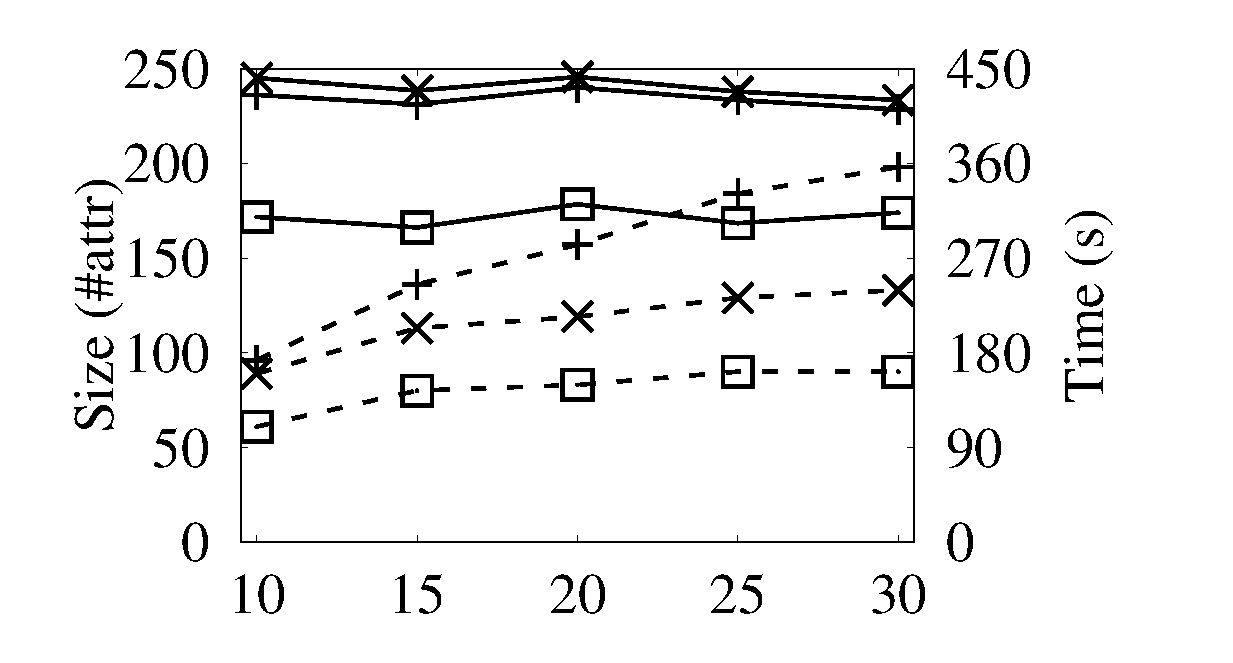
\includegraphics[width=1\textwidth]{fig/vary_q_tpch.eps}
			\begin{center}
				\vspace{-2ex}\caption{\tpch: varying $|\Q|$}
				\label{tpch-1-varyQ}
			\end{center}
			\vspace{-1ex}
        \end{subfigure}
        \hspace{-3ex}
		%
        \begin{subfigure}[b]{0.256\textwidth}
          \centering
          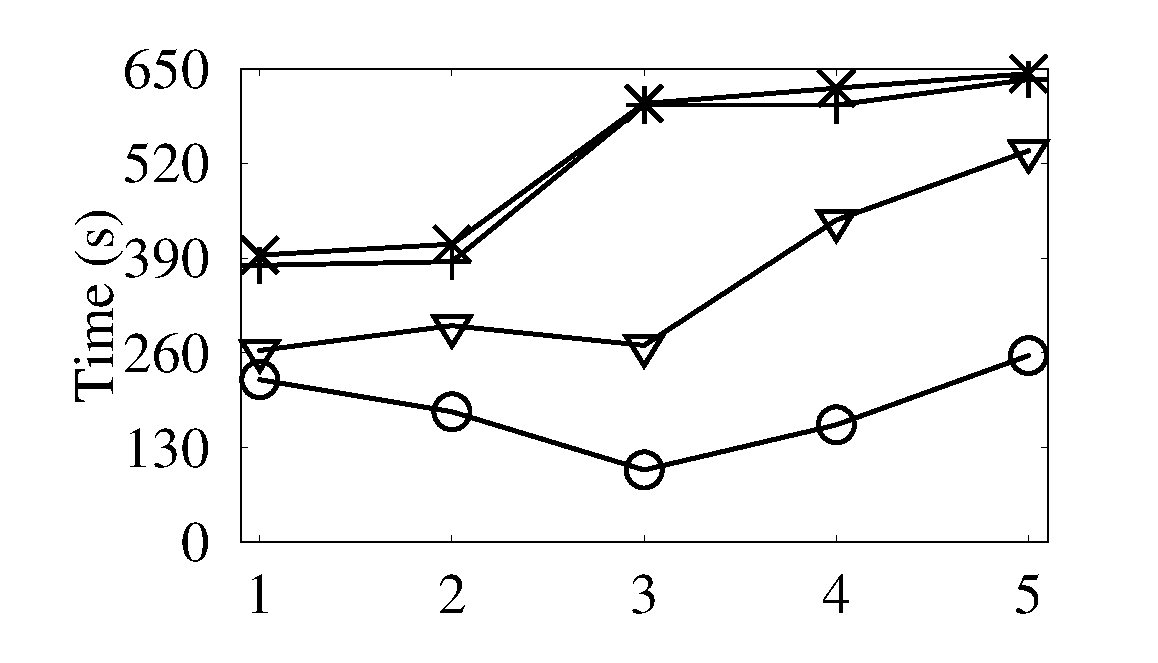
\includegraphics[width=1\textwidth]{fig/vary_j_tpch.eps}
          \begin{center}
            \vspace{-2ex}\caption{\tpch: varying \#-\at{join}}
            \label{tpch-1-vary-join}
          \end{center}
          \vspace{-1ex}
        \end{subfigure}
        \hspace{-2.8ex}
        %
  		\begin{subfigure}[b]{0.256\textwidth}
          \centering
          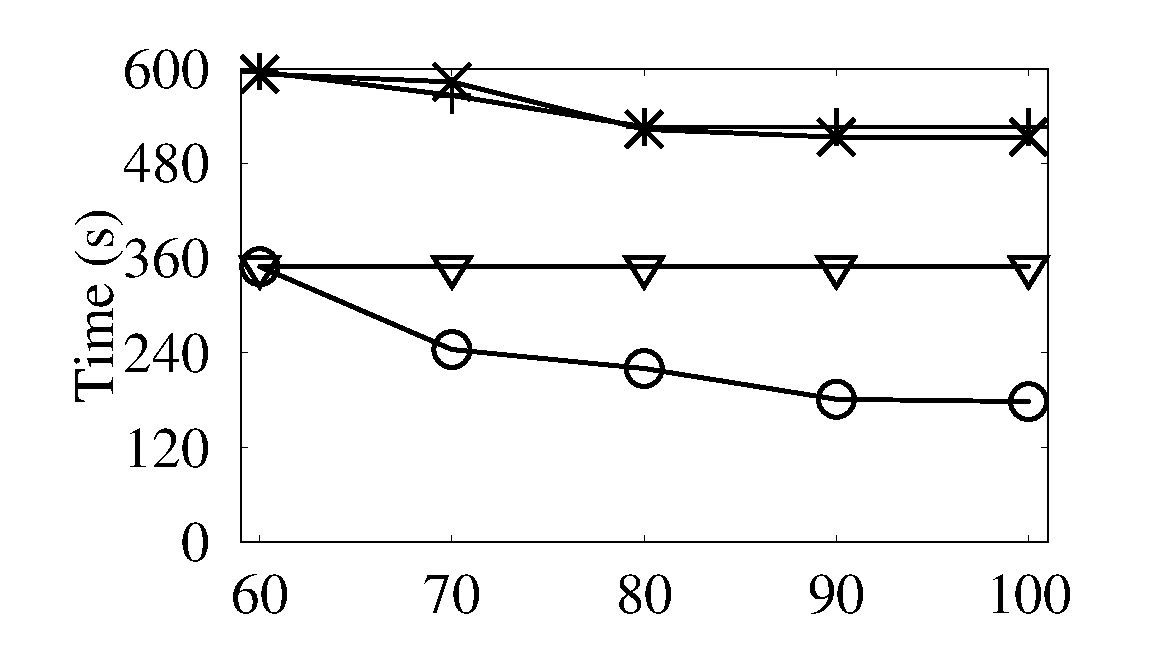
\includegraphics[width=1\textwidth]{fig/vary_b_tpch.eps}
          \begin{center}
            \vspace{-2ex}\caption{\tpch: varying $B$ (\%$B_{\at{max}}$)}
            \label{tpch-1-varyB}
          \end{center}
          \vspace{-1ex}
        \end{subfigure}
        \hspace{-2.8ex}
        %
  		\begin{subfigure}[b]{0.256\textwidth}
          \centering
          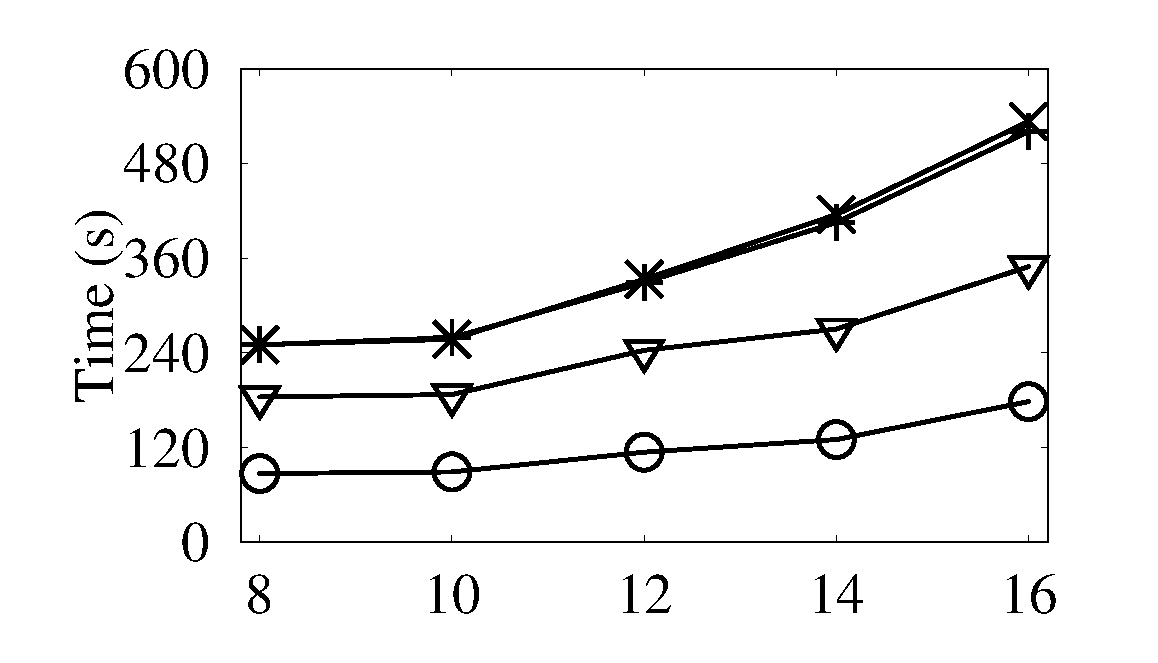
\includegraphics[width=1\textwidth]{fig/vary_d_tpch.eps}
          \begin{center}
            \vspace{-2ex}\caption{\tpch: varying $|\D|$}
            \label{tpch-1-varyD}
          \end{center}
          \vspace{-1ex}
        \end{subfigure}

        \begin{subfigure}[b]{0.271\textwidth}
			\centering
			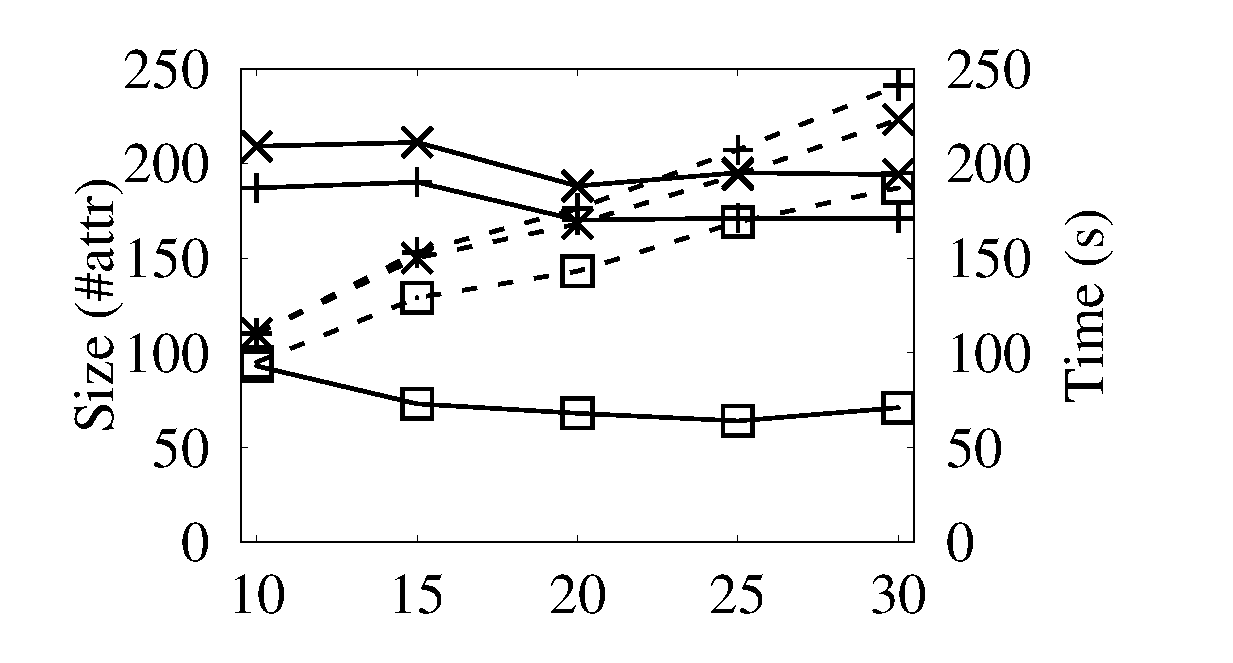
\includegraphics[width=1\textwidth]{fig/vary_q_tpcds.eps}
			\begin{center}
				\vspace{-2ex}\caption{\tpcds: varying $|\Q|$}
				\label{tpcds-1-varyQ}
			\end{center}
			\vspace{-1ex}
        \end{subfigure}
        \hspace{-3ex}
		%
        \begin{subfigure}[b]{0.256\textwidth}
          \centering
          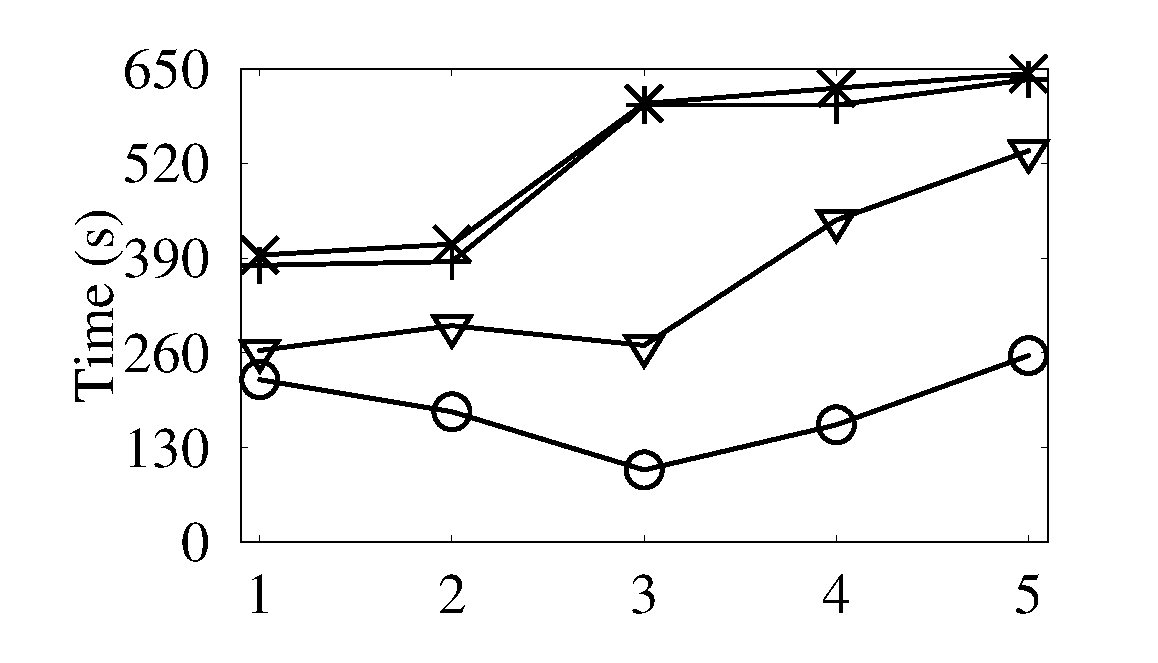
\includegraphics[width=1\textwidth]{fig/vary_j_tpch.eps}
          \begin{center}
            \vspace{-2ex}\caption{\tpcds: varying \#-\at{join}}
            \label{tpcds-1-vary-join}
          \end{center}
          \vspace{-1ex}
        \end{subfigure}
         \hspace{-2.8ex}
        %
  		\begin{subfigure}[b]{0.256\textwidth}
          \centering
          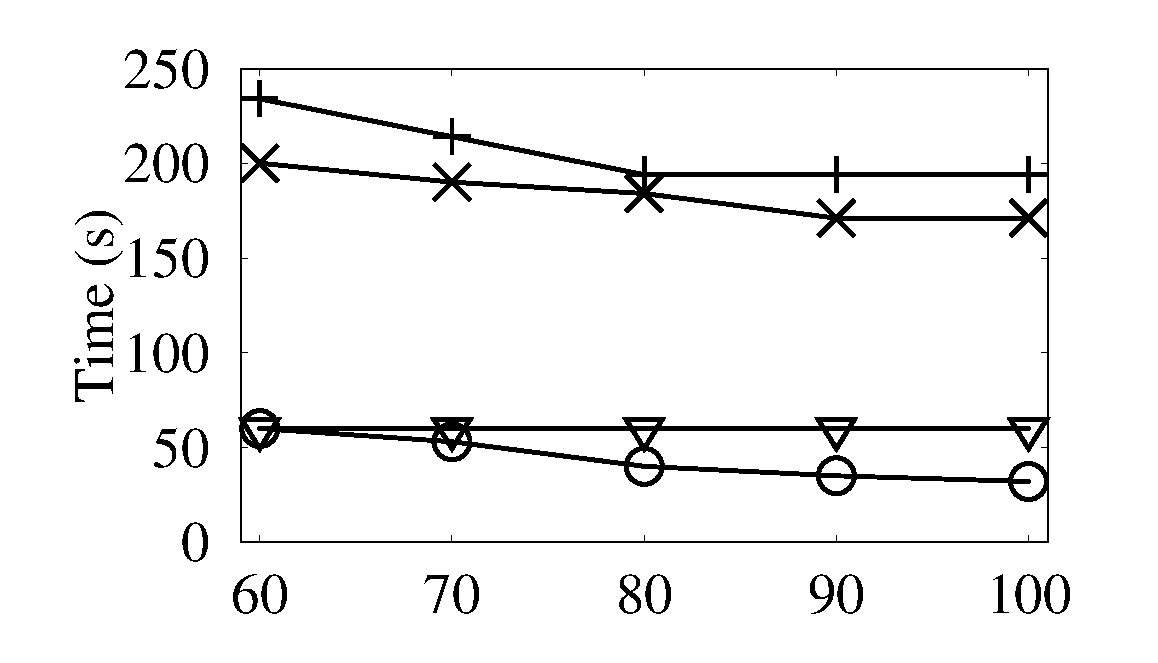
\includegraphics[width=1\textwidth]{fig/vary_b_tpcds.eps}
          \begin{center}
            \vspace{-2ex}\caption{\tpcds: varying $B$ (\%$B_{\at{max}}$)}
            \label{tpcds-1-varyB}
          \end{center}
          \vspace{-1ex}
        \end{subfigure}
         \hspace{-2.8ex}
        %
  		\begin{subfigure}[b]{0.256\textwidth}
          \centering
          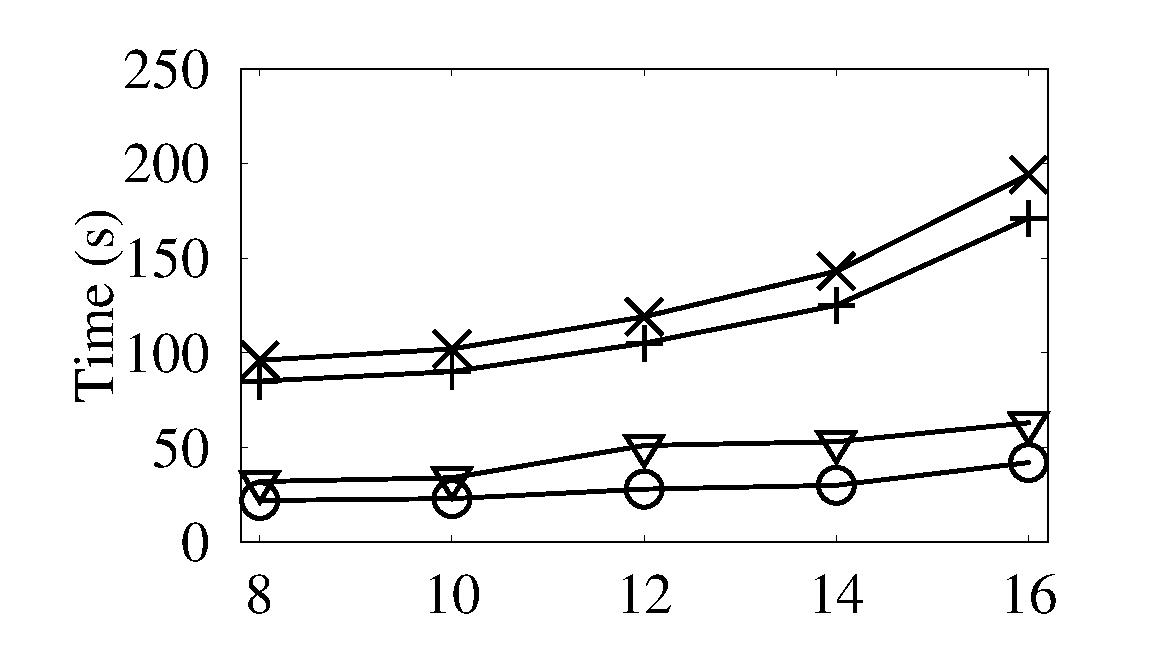
\includegraphics[width=1\textwidth]{fig/vary_d_tpcds.eps}
          \begin{center}
            \vspace{-2ex}
           \caption{\tpcds: varying $|\D|$}
            \label{tpcds-1-varyD}
          \end{center}
          %\vspace{-3.4ex}
        \end{subfigure}
\end{subfigure}
\vspace{-4.0ex}
\caption{Quality evaluation of the computed \bdss ({\bf Exp-3})}
\label{exp-quality}
\vspace{-2.5ex}
\end{figure*}

%%%%%%%%%%%%%%%




\warn{\eetitle{Implementation}.
We used SparkSQL v2.4.0 over Cassandra v3.11.6 as the \kv
system with \SQL evaluation support.
We built the sibling databases according to the computed \bdss by
all the methods, and carried out query evaluation over the
sibling \baav databases using the algorithms of \cite{VLDB19}.
In particular, each \bs $\kb{R}\bschema{X}{Y}$ is
implemented in Cassandra as a table with both $XY$ as the key
such that (a) attributes $X$ must precede $Y$ in the keys and
(b) keys are sorted by $X$. This is a lightweight implementation
of the \baav schemas with Cassandra and does not require
any modification to Cassandra.
However, its performance is actually slower than a hack-in
implementation of the \baav model inside Cassandra since
locating the keys for a given $X$-value would incur $O(\log n)$
complexity instead of $O(1)$ asymptotically, assuming there are
$n$ $XY$-values in the relation. This will favor the competitors
when compared to the default SparkSQL-over-Cassandra (tuple-as-a-value model).}


\eetitle{Configuration}.
The experiments were conducted on \warn{a Linux server with \xx CPU,
  \xx GB of memory and \xx GB of HDD disk}.
The server works as both a computing node and a storage node, \ie it works
as a Spark master/slave for the SQL layer (with \xx GB of memory) and also holds a
Cassandra partition for the storage (also with \xx GB of memory).
By default, we set the storage budget $B_{\at{max}}$ of the
\bdss to be 0.7 times of the size of the \imdb database
and 2.5 times for \tpch.
%where size is measured by the number of attributes in our case (other
%more sophisticated size measures can be adopted similarly).
All the tests were run 3 times. The average is reported here.
\looseness = -1






\stitle{Experimental Results}. We next report our findings.

\warn{\stitle{Exp-1: Benchmark tests}. Using default settings, we
first compared the benchmark query performance over \baav
schemas computed by our algorithms and over the conventional
tuple-as-a-value relations. The results are reported in
Table~[\xx]}%\ref{tab-benchmark}.



\warn{\stitle{Exp-2: Scan-free evaluation}.
We then evaluated the effectiveness of scan-free evaluation and
studied the impact of degrees on scan-free queries.}






\stitle{Exp-3: Quality of \bdss}.
We evaluated the quality of the \bdss found by each method in %under
all settings. 


\eetitle{(1) Varying $|\Q|$}. We first compared the minimum
normalized \bdss that can be computed by our method
% with rank functions $f^{(a)}$ and $f^{(b)}$,
and baselines \qcssel and \uscsel.
More specifically, 
let $\Q$ consist of all parametric queries for each benchmark;
we varied the size $|\Q|$ of $\Q$ by randomly sampling queries
from $\Q$ such that $|\Q|$ varies from \warn{10} to \warn{30} for both \tpch and \tpcds. For each $\Q$, we compare the quality of
the minimum \bds $\kb{\R}$ found by each method such that
$\kb{\R}$ is in the normal form for $\Q$ (for our method, we
only need to keep $f_{3}$ in the objective function of \opts,
\ie $c_{i} = 0$ for $i\ak\in\ak \{1,\ak 2,\ak 4\}$).
%(b) $\Q$ is scan-free over $\kb{\R}$.
We assess the quality of such \bdss by (a) their sizes and (b) the
query evaluation time over them.

\sstab (a) As shown by the left $y$-axis of Figures
\ref{tpch-1-varyQ} and \ref{tpcds-1-varyQ}, 
among all methods, our method (shown as \opts)
%with rank function $f^{(b)}$
generates the minimum \bdss that are in the normal
form,
%for the queries,
in all cases. For example, the size of the
minimum normalized \bds computed by \warn{\uscsel} is
\warn{1.57} and \warn{1.15} times larger than our method
%with rank function $f^{(b)}$
when $|\Q| = \warn{10}$ for \tpch
and \tpcds, respectively; it increases to \warn{2.20} and \warn{1.28} times when
$|\Q| = \warn{30}$.
%The minimum normalized \bds computed by our method
%with $f^{{(a)}}$  is slightly larger than our
%method with $f^{(b)}$, but is still on average \xx times smaller
%than those computed by \uscsel.
The results for \qcssel are similar. %to that of \uscsel. 


\sstab (b) For each query $Q$, we define the speedup by method
$A$ over method $B$ as the ratio of the evaluation time of $Q$
on the minimum normalized \bds computed by method $A$ over that
by method $B$; naturally, the average speedup of $\Q$ by method
$A$ over method $B$ is the average of the speedups of queries in
$\Q$ by $A$ over $B$.
As shown by the right $y$-axis of Figures \ref{tpch-1-varyQ} and \ref{tpcds-1-varyQ},
when $|\Q|$ varies from \warn{10} to \warn{30} for
\tpcds, the average speedup by our method
%with rank function $f^{(a)}$
\warn{is \warn{6.31} (resp.~\warn{4.00}) times over algorithm \qcssel
  (resp.~\uscsel) on average, up
to \warn{7.68} (resp. \warn{5.05}) times.}
The results over \tpch are similar.

\vspace{1ex}
These show that our method can find normalized \bdss that are of
smaller size than those found by the baselines (\eg on average \warn{1.43}
times smaller) and %but
provide even faster query evaluation
performance (\eg on average \warn{3.81} times faster).






\eetitle{(2) Varying query complexity (\#-\at{join})}.
We then evaluated the ability of all methods to process complex
queries, \ie queries with varying number of %many
joins. We
classified queries $\Q$ of each benchmark into 5 sub-workloads
$\Q_{i}\ak (i\ak\in\ak [1,\ak 5])$, 
where $\Q_{i}$ consists of all parametric queries in $\Q$ that have exactly $i$
joins. We set the storage budget $B$ to $B_{\at{max}}$ and tested the average
speedup for each sub-workloads in the same ways as in EXP-1(1b)
above. In particular, when a \bds is not in the normal form of a
query $Q$, we evaluate $Q$ directly on the original database and
use the evaluation time to calculate the speedup for $Q$.
For our method, we tested it with both rank functions $f^{(a)}$
and $f^{(b)}$.
\looseness = -1

\vspace{0.6ex}
The results for \tpch and \tpcds are shown in
Figures~\ref{tpch-1-vary-join} and \ref{tpcds-1-vary-join},
respectively. The results tell us the following. 

\sstab (a) Our method works at its best with rank
function $f^{(a)}$ in %terms of the
query performance.
The average query speedup achieved by our method
with rank function $f^{(a)}$ over %it
with
$f^{(b)}$ is \warn{2.14} and \warn{2.52} times on average for \tpch and \tpcds,
respectively, up to \warn{4.71} and \warn{27.96} times.
Moreover, no matter with which rank function, it always
provides \bdss better than both \qcssel and \uscsel do.
For example, with $f^{(a)}$ it is on average \warn{5.57} and \warn{11.36}
times better than \qcssel over \tpch and \tpcds, respectively,
up to \warn{34.76} and \warn{71.40} times; for $f^{(b)}$ it is \warn{3.10} and
\warn{6.38} times on average, respectively, up to \warn{19.92} and \warn{35.97} times.
%the numbers for $f^{(b)}$ are \xx and
%\xx times on average, up to \xx and \xx times.
\looseness = -1

\sstab (b) Our method with both rank functions $f^{(a)}$ and
$f^{(b)}$ are able to handle complex queries much better than
the baselines, and the gap gets bigger when the number
of joins (\#-\at{join}) increases.
For instance, when \#-\at{join} increases from \warn{1} to \warn{5} over
\tpcds, the average speedup by our method with $f^{(a)}$ over
\qcssel increases from \warn{15.26} to \warn{17.05} times; the gap is \warn{1.63} and \warn{16.91}
times over \uscsel; the results are similar for \tpch.


\sstab (c) However, this comes with a price: the maintenance cost
of the \bdss computed by our method with $f^{(a)}$ is \warn{4.04} times
larger than the cost with $f^{(b)}$ on average,
where the cost is measured by $\update(\Q, \kb{\R})$ (recall Section~\ref{sec-rank}). 


\eetitle{(3) Varying space budget $B$}. We next evaluated the
quality of \bdss computed by our method under varying storage
budget $B$. Varying $B$ from \warn{60}\%$B_{\at{max}}$ to
$B_{\at{max}}$, we compared the average evaluation time per query
of all methods. We used all parametric queries for each
benchmark.
% When the size of the
% \bdss $\kb{\R}$ identified by the baseline algorithms
% exceeds the space budget $B$, we remove \bss in $\kb{\R}$ that has
% the fewest number of attributes until $\size(\Q, \kb{\R})\leq B$;
% if the reduced $\kb{\R}$ is not in the normal form for $\Q$
% anymore, we return \texttt{err} and remove them when calculating
% the average query evaluation time for the baselines. 
The results for \tpch and \tpcds are reported in
Figures~\ref{tpch-1-varyB} and \ref{tpcds-1-varyB}.
We observed the following.

\sstab (a) Consistent with Exp-1(1a), our method with both
rank functions is able to identify \bdss that
are in the normal form under small space budget $B$,
while the baselines cannot.

\sstab (b) Queries are answered more efficiently on \bdss
computed by our method than over those found by the baselines,
for both rank functions.
Moreover, the gaps become even larger when $B$ is
smaller. For example, the average speedup by our method with
rank function $f^{(a)}$ over algorithm \qcssel is on average \warn{4.44}
times, and up to \warn{34.76} times over \tpch; the speedup is %speedups are
\warn{8.56} times
on average over \tpcds, up to \warn{71.40} times.
\looseness = -1

\sstab (c) Consistent with other experiments reported
above, our method works \warn{better with rank
function $f^{(a)}$ than with $f^{(b)}$}
in terms of query evaluation performance.
Moreover, the larger $B$ becomes, the bigger the gap is. 
For example, when $B$ increases from \warn{60}\%$B_{\at{max}}$ to
$B_{\at{max}}$, the speedup by
our method with $f^{(a)}$ over with $f^{(b)}$ \warn{increases} from \warn{1.05}
to \warn{2.14} times over \tpch. 



\eetitle{(4) Varying dataset size}.
We finally evaluated the quality of the \bdss by testing them
with datasets of different sizes. We
varied the size of the datasets $D$ from \warn{8}GB to \warn{16}GB and
compared the query evaluation time in the same setting
of EXP-1(3) above,
except that  $B$ is fixed to $B_{\at{max}}$ instead.
The results over \tpch and \tpcds are reported in
Figures~\ref{tpch-1-varyD} and \ref{tpcds-1-varyD}, respectively.
Consistent with other experiments, our method with $f^{(a)}$ computes the best
\bdss in terms of query evaluation performance, and its gap over
others increases when the dataset grows bigger, \eg
from \warn{5.97} to \warn{7.13} times when the \tpcds dataset increases from \warn{8} GB to \warn{16} GB.


%%%%%%%%%%%%%%%%% EXP-2
\begin{table}
  \begin{center}
    \begin{footnotesize}
      \caption{Efficiency of our method (\opts and \usc) ({\bf
          Exp-2}) (\textnormal{\footnotesize $\kb{\R}$ is the \bds returned by
          \opts; $\kb{\A}$ is the universe set computed by \usc;
          the evaluation time includes that of both \opts and \usc}) \label{exp-2}}
      \setlength{\aboverulesep}{0.1pt}
      \setlength{\belowrulesep}{0.5pt}
      \setlength{\tabcolsep}{2ex} % for the horizontal padding
      \renewcommand{\arraystretch}{1.1}% for the vertical padding
      %\vspace{-0.7ex}
      \hspace*{-0.8ex}\begin{tabu}{l|[0.30mm]l|[0.15mm]l|[0.15mm]l|[0.30mm]l|[0.15mm]l|[0.15mm]l}
        \toprule
        \multirow{2}{*}{\bf $f(\Q, \kb{\R})$} & \multicolumn{3}{c|[0.30mm]}{\textbf{TPC-H}} & \multicolumn{3}{c}{\textbf{TPC-DS}} \\\cline{2-7}
        & \multicolumn{1}{c|}{$|\kb{\R}|$} & \multicolumn{1}{c|}{$|\kb{\A}|$} & \multicolumn{1}{c|[0.30mm]}{time} & \multicolumn{1}{c|}{$|\kb{\R}|$} & \multicolumn{1}{c|}{$|\kb{\A}|$}   & \multicolumn{1}{c}{time}  \\\midrule
        $f^{(a)}$ &  149& 272&  0.42& 271& 376 & 0.27\\\hline
        $f^{(b)}$ &  91& 272&  0.39& 187& 376 & 0.23\\\bottomrule
      \end{tabu}
    \end{footnotesize}
  \end{center}
  \vspace{-3.4ex}
\end{table}
%%%%%%%%%%%%%%%%% 

%\vspace{0.36ex}
\stitle{Exp-4: Efficiency}.
We also evaluated the efficiency of our method.
We used the same setting as EXP-1(4) and tested
%We used all queries for both benchmarks and tested
(a) the size $|\kb{\A}|$ of the universe set $\kb{\A}$ computed by \usc;
(b) the size $|\kb{\R}|$ of the final \bds $\kb{\R}$ returned by \opts; and
(c) the total time taken by our method (\ie \opts and \usc).
%for computing $\kb{\R}$.
The results of our algorithms
%with both rank functions
are reported in Table~\ref{exp-2}. It shows that our algorithms are
efficient, and the universe set is of moderate size while being
able to cover the optimal \bdss. 


\stitle{Summary}. From the experimental study we find the following.
  (1)  The \bdss computed by our algorithms are effective.
  Over the computed  \bdss with SparkSQL-over-Cassandra,
  on average \tpch and \tpcds queries can be made \warn{4.28} and \warn{7.01}
 times faster than over the \bdss computed by the baselines,
 respectively.
 %and \xx and \xx times faster than executing directly
 %over relations stored under
 %the conventional tuple-as-a-value model in Cassandra.
 (2) Moreover, the gap increases when the queries are more
 complex (\ie with more joins) or the datasets grow bigger.
 (3) \warn{Our algorithms are efficient: they finish in
 0.42 and 0.27 seconds for \tpch and \tpcds, respectively.}


\eat{%EAT
  \begin{figure*}[tb!]
%\vspace{-1.7ex}
\begin{subfigure}[b]{1.00\textwidth}
  \centering
        \begin{subfigure}[b]{0.245\textwidth}
			\centering
			
\includegraphics[width=1\textwidth]{fig/a.eps}
			\begin{center}
				\vspace{-2ex}\caption{\tpch: varying $|\Q|$}
				\label{tpch-1-varyQ} 
			\end{center}
			\vspace{-1ex}
        \end{subfigure}
        %\hspace{-2.2ex}
		%
        \begin{subfigure}[b]{0.245\textwidth}
          \centering
          
\includegraphics[width=1\textwidth]{fig/a.eps}
          \begin{center}
            \vspace{-2ex}\caption{\tpch: varying \#-\at{join}}
            \label{tpch-1-vary-join} 
          \end{center}
          \vspace{-1ex}
        \end{subfigure}
        % \hspace{-2.2ex}
        %
  		\begin{subfigure}[b]{0.245\textwidth}
          \centering
          
\includegraphics[width=1\textwidth]{fig/a.eps}
          \begin{center}
            \vspace{-2ex}\caption{\tpch: varying $B$}
            \label{tpch-1-varyB} 
          \end{center}
          \vspace{-1ex}
        \end{subfigure}
        % \hspace{-2.2ex}
        % 
  		\begin{subfigure}[b]{0.245\textwidth}
          \centering
          
\includegraphics[width=1\textwidth]{fig/a.eps}
          \begin{center}
            \vspace{-2ex}\caption{\tpch: varying $|\D|$}
            \label{tpch-1-varyD} 
          \end{center}
          \vspace{-1ex}
        \end{subfigure}

        \begin{subfigure}[b]{0.245\textwidth}
			\centering
			
\includegraphics[width=1\textwidth]{fig/a.eps}
			\begin{center}
				\vspace{-2ex}\caption{\tpcds: varying $|\Q|$}
				\label{tpcds-1-varyQ} 
			\end{center}
			\vspace{-1ex}
        \end{subfigure}
        %\hspace{-2.2ex}
		%
        \begin{subfigure}[b]{0.245\textwidth}
          \centering
          
\includegraphics[width=1\textwidth]{fig/a.eps}
          \begin{center}
            \vspace{-2ex}\caption{\tpcds: varying \#-\at{join}}
            \label{tpcds-1-vary-join} 
          \end{center}
          \vspace{-1ex}
        \end{subfigure}
        % \hspace{-2.2ex}
        %
  		\begin{subfigure}[b]{0.245\textwidth}
          \centering
          
\includegraphics[width=1\textwidth]{fig/a.eps}
          \begin{center}
            \vspace{-2ex}\caption{\tpcds: varying $B$}
            \label{tpcds-1-varyB} 
          \end{center}
          \vspace{-1ex}
        \end{subfigure}
        % \hspace{-2.2ex}
        % 
  		\begin{subfigure}[b]{0.245\textwidth}
          \centering
          
\includegraphics[width=1\textwidth]{fig/a.eps}
          \begin{center}
            \vspace{-2ex}\caption{\tpcds: varying $|\D|$}
            \label{tpcds-1-varyD} 
          \end{center}
          \vspace{-1ex}
        \end{subfigure}
      \end{subfigure}
\caption{Quality evaluation of the computed \bdss ({\bf Exp-1})}
\label{exp-quality}
\end{figure*}
    

\section{Experimental Study}
\label{sec-expt}

Using standard benchmarks, we conducted two sets of experiments to evaluate
(1) the quality of \bdss computed by our algorithms; and
(2) the efficiency of our algorithms.


\stitle{Experimental Settings}. We start with the settings.

\eetitle{Benchmarks}. We used two standard benchmarks
\tpch~\cite{tpch} and \tpcds~\cite{tpcds}, including their 
data generators and built-in parametric queries.
(1) \tpch generates data using {\small TPC-H}
\kw{dbgen}~\cite{tpch}, with 8 relations. It has 22 built-in
parameterized \SQL queries.
(2) \tpcds generates data using {\small
TPC-DS} \kw{dbgen}~\cite{tpcds}, with 24 relations. It has 99
built-in parametric \SQL queries.
By default, we evaluated the query evaluation performance over
datasets of 16GB for both benchmarks. 

For each relation in the benchmark databases, we assign a random
update frequency in the range of [1, 10] for testing the
incremental maintenance cost of the generated \bdss. 


\eetitle{Parametric queries}. We used all built-in
parameterized queries of both benchmarks. When a query is not
\SPC, we used its \SPC sub-queries instead. After this, we have
\xx and \xx\ parametric \SPC\ \tpch and \tpcds queries, respectively (only
16 \tpch queries contain sensible \SPC sub-queries with
selections); all of them are K-FK join only queries. To evaluate
with larger workloads and varying query complexities, we also
generated \xx and \xx parametric \SPC queries for \tpch and \tpcds,
respectively, with the number of joins varying from \warn{0} to
\warn{3}.


We assign a random frequency $w_{Q}$ in the range of [1, 1000] to each
parametric query $Q$. In our tests, when evaluate the total
evaluation time of a query workload, we multiply the (average)
evaluation time of each query by its frequency and then sum up
over all the queries in the workload; this helps reduce the total
test time by avoiding executing a query for, \eg up to 1000
times, while still providing an accurate overall execution time.
\looseness = -1


\eetitle{Aggregate ranking functions}.
In our test, we focus on computing the best \bdss subject to a
storage budget $B$. Therefore, we treat the space cost (\ie
measure (3)) as a constraint in the ILP programs of algorithm
\opts (Section~\ref{sec-select}). For convenience, we used the
number of total attributes to measure the space cost of the
\bdss; note that this is not a restriction of our approach as the
measures and algorithms treat the estimated space cost as input
and hence support any more sophisticated space cost estimation
for measure (3) as an input.


We used four aggregate ranking functions $f(\Q, \kb{\R}) = c_{1}f_{1} +
c_{2}f_{2} + c_{3}f_{3} + c_{4}f_{4}$ (recall
Section~\ref{sec-rank}), where 
\bi
\item[(a)] $f^{(a)}(\Q, \kb{\R})$: $c_{1} = 1$, $c_{i} = 0(i\in [2,4])$.
\item[(b)] $f^{(b)}(\Q, \kb{\R})$: $c_{1} = 0.9999$ and $c_{2} = 0.0001$. 
\item[(c)] $f^{(c)}(\Q, \kb{\R})$: $c_{1} = 0.01$, $c_{2} = 0.0001$ and $c_{4}
  = 0.9899$. 
\item[(d)] $f^{(d)}(\Q, \kb{\R})$: $c_{1} = 0.9899$, $c_{2} =
  0.0001$ and $c_{4} = 0.01$.
\ei
Intuitively, $f^{(a)}$ is to compute the \bdss that can make the
largest number of queries bounded, by using measure (1) only; 
$f^{(b)}$ is to enhance measure (1) with measure (2), to further
improve the performance of queries over the optimal \bdss;
$f^{(c)}$ is to give priority to the maintenance cost, \ie
measure (4); and $f^{(d)}$ is to give priority to the performance
of queries over the \bdss while also taking into account the
incremental maintenance with a lower priority.

Observe that the four aggregate ranking functions above models
four scenarios in practice: if one concerns the number of queries
with the scan-free evaluability property, then $f^{(a)}$ is the
one to go; if one wants to additionally maximize the performance
gains, then $f^{(b)}$ gives more control on the \bdss; if one
additionally considers incremental maintenance cost but is less
important than query evaluation performance, then $f^{(d)}$ fits
best; if one cares incremental performance most, then $f^{(c)}$
captures the objective best with all three measures taken
together.
\looseness = -1


\eetitle{Algorithms}. We implemented our algorithms \opts
(Section~\ref{sec-select}) and \usc (Section~\ref{sec-cover}). We
used Gurobi~\cite{gurobi} to solve ILP-(I) and ILP-(II) of \opts.
In particular, when implementing \usc, we lifted the restriction
on the size of $\Sigma$ of procedure \decompose (see the remark
at the end of Section~\ref{sec-cover}). This allows \usc to
generate a larger universe set for \opts; as will be shown
shortly, the our approach is still efficient. 

\vspace{0.7ex}
We also designed two baselines.

\vspace{-0.4ex}
\etitle{(1) Algorithm \qcssel} that simply returns the collection
of all \qcs of all queries as the schemas, under the
tuple-as-a-value model; that is, it treats each \qcs $W$ as a \bs
$\bschema{\at{id}}{W}$, where $\at{id}$ is an id attribute (or
the candidate key) for $W$.

\vspace{-0.4ex}
\etitle{(2) Algorithm \uscsel} that returns $\kb{\R}$ for
consisting of $\kb{R}_{Q}^{1}$ generated in Step (1)
of \usc (Section~\ref{sec-cover}) for each query $Q$.

\vspace{0.4ex}
Note that, the \bdss selected by both baselines are in the normal
form for the query workload. 

\eetitle{Configuration}.
The experiments were conducted on a cluster of \warn{4} Amazon
EC2 \warn{m4.2xlarge} instances, with \warn{32}GB of memory, \warn{8}
vCPUs and \warn{500}GB of NVMe SSD for each instance.
We used \warn{SparkSQL v\xx over Cassandra v\xx} as the \kv
system with \SQL evaluation support.
We built the sibling databases according to the computed \bdss by
all the methods, and carried out query evaluation over the
sibling \baav databases by following \cite{VLDB19}. 
Each EC2 instance works as both a computing node and a storage node, \ie it works
as a Spark master/slave for the SQL layer and also holds a
Cassandra partition for the storage (with a dedicated Spark
master node).
% We also used one additional instance as the Spark master.
All the tests were run 3 times. The average is reported here.


\stitle{Experimental Results}. We next report our findings.

\stitle{Exp-1: Quality of \bdss}.
We evaluated the quality of the \bdss found by every method under
every setting. 

\eetitle{(1) Varying $|\Q|$}. We first assess the quality of the
computed \bdss by evaluating the average query evaluation time
per each instantiated query over query workloads of varying sizes.
More specifically, let $\Q$ consists of all parametric queries
for each benchmark; we varied the size $|\Q|$ of $\Q$ by randomly
sampling queries from $\Q$ such that $|\Q|$ varies from \xx to
\xx for \tpch and \xx to \xx for \tpcds. We set the space budget
$B$ to the total number $B_{\at{max}}$ of attributes in the database schema of
each benchmark, \ie the generated \bdss are no larger than the
original database schemas. For both \tpch and \tpcds, we generate
database instances of size \xx GB. We instantiated each
parametric query by randomly drawing values from the database
instances for the parameters. To save time, for each parametric
query $Q$, we evaluated five queries instantiated from $Q$ and
used their average evaluation time as the evaluation time $t_{Q}$
for $Q$. For a workload $\Q$, we calculated the average evaluated
time per query as $\sum_{Q\in \Q} w_{Q}*t_{Q}/\sum_{Q\in \Q}w_{Q}$.

The results for \tpch and \tpcds are reported in
Fig.~\ref{tpch-1-varyQ} and \ref{tpcds-1-varyQ}, respectively.
We found the following. 

\sstab (a) All \bdss generated by all methods are in the normal
form and hence all queries can be answered. 

\sstab (b) Our method with ranking function $f^{(b)}$
consistently generated \bdss over which queries are answered the
most efficiently. This followed by our method with ranking
function $f^{(d)}$. Baseline \qcssel is the worst.
For example, 


\sstab (c) The larger $|\Q|$ is, the better our method performs
when compared to the baselines. For example, 


\sstab (d) In particular, while ranking function $f^{(c)}$ gives
the large majority of weight (98.99\%) to minimizing incremental
maintenance cost, with out algorithms it still identifies \bdss
that are more efficient then baseline \qcssel while yielding
smaller maintenance cost at the same time. 
For example, 


\eetitle{(2) Varying query complexity (\#-\at{join})}.
We then evaluated the ability of all methods to process complex
queries, \ie queries with many joins. More specifically, we
classified queries of each benchmark workload $\Q$ into 4 sub-workloads
$\Q_{1}$, $\Q_{2}$, $\Q_{3}$ and $\Q_{4}$, where $\Q_{i}$
consists of all parametric queries in $\Q$ that have exactly $i$
joins. We set the space budget $B$ and tested the average
evaluation time per each instantiated query of each sub-workloads
in the same ways as in EXP-1(1) above.

The results for \tpch and \tpcds are shown in
Fig.~\ref{tpch-1-vary-join} and \ref{tpcds-1-vary-join},
respectively. They tell us the following. 

\sstab (a) Our methods deal with complex queries much better than
the baselines and the gap increases when the number of joins
(\#-\at{join}) increases. 
For instance, 

\sstab (b) Our method with ranking function $f^{(b)}$ works at
its best in terms of the average query evaluation time. In
particular, its gaps over our method with ranking functions
$f^{(c)}$ and $f^{(d)}$ becomes larger when \#-at{join} increases.
For instance, 


\sstab (c) However, this comes with a price: the maintenance cost
of the \bdss computed by our method with $f^{(b)}$ is \xx times
larger than it with $f^{(c)}$, where the cost is measured by
$\update(\Q, \kb{\R})$ (recall Section~\ref{sec-rank}). 
For instance, 


\eetitle{(3) Impact of space budget $B$}. We next evaluated the
quality of \bdss computed by our method under varying storage
budget $B$. Varying $B$ from 40\%$B_{\at{max}}$ to
$B_{\at{max}}$, we compared the average evaluation time per query
of all methods. We used all parametric queries for each
benchmark. When the \bdss $\kb{\R}$ identified by the baseline algorithms
exceeds the space budget $B$, we remove \bss in $\kb{\R}$ with
the fewest number of attributes until $\size(\Q, \kb{\R})\leq B$;
if the reduced $\kb{\R}$ is not in the normal form for $\Q$
anymore, we return \texttt{err} and remove them when calculating
the average query evaluation time for the baselines. 
The results for \tpch and \tpcds are given in
Fig.~\ref{tpch-1-varyB} and \ref{tpcds-1-varyB}.
We observed the following.

\sstab (a) Our method with all four ranking functions can
identify \bdss that are in the normal form under small space
budget $B$ when the baselines cannot.
For example, 


\sstab (b) Queries are answered more efficiently on \bdss
computed by our methods than over those find by the baselines,
for all ranking functions.  Moreover, the gaps are even larger
when $B$ is smaller. For example, 


\sstab (c) Consistent with other experiments, our method works
best with ranking function $f^{(b)}$ in terms of the average
query evaluation time. For example, 


\eetitle{(4) Varying dataset size}.
We finally evaluated the quality of the \bdss by testing them
with varied size of datasets. More specifically, we varied the
size of the datasets from 4GB to 16GB and compared the average
query evaluation time following the setting of EXP-1(3) above
with $B$ fixed to $B_{\at{max}}$ instead.
The results for \tpch and \tpcds are reported in
Fig.~\ref{tpch-1-varyD} and \ref{tpcds-1-varyD}, respectively.
They tell us that our method with $f^{(b)}$ computes the best
\bdss in terms of query evaluation performance, and its gap over
others increases when the dataset grow. For example, 


%%%%%%%%%%%%%%%%% EXP-2
\begin{table}
  \begin{center}
    \begin{footnotesize}
      \caption{Efficiency of our method (\opts and \usc) ({\bf
          Exp-2}) (\textnormal{\footnotesize $\kb{\R}$ is the \bds returned by
          \opts; $\kb{\A}$ is the universe set computed by \usc;
          the evaluation time includes that of both \opts and \usc}) \label{exp-2}}
      \setlength{\aboverulesep}{0.1pt}
      \setlength{\belowrulesep}{0.5pt}
      \setlength{\tabcolsep}{1.5ex} % for the horizontal padding
      \renewcommand{\arraystretch}{1.08}% for the vertical padding
      \hspace*{-0.8ex}\begin{tabu}{l|[0.30mm]l|[0.15mm]l|[0.15mm]l|[0.30mm]l|[0.15mm]l|[0.15mm]l}
        \toprule
        \multirow{2}{*}{\bf $f(\Q, \kb{\R})$} & \multicolumn{3}{c|[0.30mm]}{\textbf{TPC-H}} & \multicolumn{3}{c}{\textbf{TPC-DS}} \\\cline{2-7}
        & \multicolumn{1}{c|}{$|\kb{\R}|$} & \multicolumn{1}{c|}{$|\kb{\A}|$} & \multicolumn{1}{c|[0.30mm]}{time} & \multicolumn{1}{c|}{$|\kb{\R}|$} & \multicolumn{1}{c|}{$|\kb{\A}|$}   & \multicolumn{1}{c}{time}  \\\midrule
        $f^{(a)}$ &  & &  & & & \\\hline
        $f^{(b)}$ &  & &  & & & \\\hline
        $f^{(c)}$ &  & &  & & & \\\hline
        $f^{(d)}$ &  & &  & & & \\\bottomrule
      \end{tabu}
    \end{footnotesize}
  \end{center}
  \vspace{-2.7ex}
\end{table}
%%%%%%%%%%%%%%%%% 


\stitle{Exp-2: Efficiency}. 
We also evaluated the efficiency of our method. 
We used all queries for both benchmarks and tested
(a) the size of the universe set $\kb{\A}$ computed by \usc;
(b) the size of the final \bds $\kb{\R}$ returned by \opts; and
(c) the total time taken by \opts and \usc for computing
$\kb{\R}$.
The results of our algorithms with all four ranking functions are
shown in Table~\ref{exp-2}. It shows that our algorithms are
efficient and the universe set is of moderate size while being
able to cover the optimal \bdss. For example,
}%EAT

%%%%%%%% Section 7 %%%%%%%%
\section{Conclusion}
\label{sec-conclude}
\vspace{-0.4ex}

We have identified, formulated and studied the \baav schema selection
problem for \kv stores. We have proposed a normal form for \baav schemas,
and come up with an aggregate rank function based on four practical
criteria. We have shown that the schema selection problem is
\NP-complete. Despite the intractability, we have developed
efficient algorithms for selecting \baav schema while warranting
optimality under practical conditions. Our experimental studied
has verified that the method is practical, as indicated by
the effectiveness of the \baav schema selected
and the efficiency of the algorithms.

One topic for future work is to learn coefficients of the aggregate
rank function (Section~\ref{sec-rank}) possibly by employing machine
learning models. Another topic is to extend the study to
support multiple query loads that run on the same \kv store at the same time.
A third topic is to implement the framework of Section~\ref{sec-schema}
to support parametric queries, based on algorithms for
schema selection and incremental maintenance of this paper
and the query plan generation algorithms of~\cite{VLDB19}.


\newpage
%\renewcommand{\baselinestretch}{0.99}
\bibliographystyle{abbrv}
\bibliography{paper}

%\balance

\end{document}



 
